% Options for packages loaded elsewhere
\PassOptionsToPackage{unicode}{hyperref}
\PassOptionsToPackage{hyphens}{url}
\documentclass[
  a4paper,
]{book}
\usepackage{xcolor}
\usepackage{amsmath,amssymb}
\setcounter{secnumdepth}{5}
\usepackage{iftex}
\ifPDFTeX
  \usepackage[T1]{fontenc}
  \usepackage[utf8]{inputenc}
  \usepackage{textcomp} % provide euro and other symbols
\else % if luatex or xetex
  \usepackage{unicode-math} % this also loads fontspec
  \defaultfontfeatures{Scale=MatchLowercase}
  \defaultfontfeatures[\rmfamily]{Ligatures=TeX,Scale=1}
\fi
\usepackage{lmodern}
\ifPDFTeX\else
  % xetex/luatex font selection
\fi
% Use upquote if available, for straight quotes in verbatim environments
\IfFileExists{upquote.sty}{\usepackage{upquote}}{}
\IfFileExists{microtype.sty}{% use microtype if available
  \usepackage[]{microtype}
  \UseMicrotypeSet[protrusion]{basicmath} % disable protrusion for tt fonts
}{}
\makeatletter
\@ifundefined{KOMAClassName}{% if non-KOMA class
  \IfFileExists{parskip.sty}{%
    \usepackage{parskip}
  }{% else
    \setlength{\parindent}{0pt}
    \setlength{\parskip}{6pt plus 2pt minus 1pt}}
}{% if KOMA class
  \KOMAoptions{parskip=half}}
\makeatother
\usepackage{longtable,booktabs,array}
\usepackage{caption}
\captionsetup[table]{skip=6pt}
\newcounter{none} % for unnumbered tables
\usepackage{calc} % for calculating minipage widths
% Correct order of tables after \paragraph or \subparagraph
\usepackage{etoolbox}
\makeatletter
\patchcmd\longtable{\par}{\if@noskipsec\mbox{}\fi\par}{}{}
\makeatother
\usepackage{graphicx}
\makeatletter
\newsavebox\pandoc@box
\newcommand*\pandocbounded[1]{% scales image to fit in text height/width
  \sbox\pandoc@box{#1}%
  \Gscale@div\@tempa{\textheight}{\dimexpr\ht\pandoc@box+\dp\pandoc@box\relax}%
  \Gscale@div\@tempb{\linewidth}{\wd\pandoc@box}%
  \ifdim\@tempb\p@<\@tempa\p@\let\@tempa\@tempb\fi% select the smaller of both
  \ifdim\@tempa\p@<\p@\scalebox{\@tempa}{\usebox\pandoc@box}%
  \else\usebox{\pandoc@box}%
  \fi%
}
% Set default figure placement to htbp
\def\fps@figure{htbp}
\makeatother
\setlength{\emergencystretch}{3em} % prevent overfull lines
\providecommand{\tightlist}{%
  \setlength{\itemsep}{0pt}\setlength{\parskip}{0pt}}
\usepackage[]{natbib}
\bibliographystyle{apalike}
\usepackage{booktabs}
\usepackage{polyglossia}
\setmainlanguage{italian}
\usepackage{xcolor}
\usepackage{pagecolor}
\definecolor{washi}{RGB}{248, 243, 214}
\pagecolor{washi}
\usepackage{bookmark}
\IfFileExists{xurl.sty}{\usepackage{xurl}}{} % add URL line breaks if available
\urlstyle{same}
% fallback for those not using the hyperref driver hyperxmp:
\makeatletter
\@ifundefined{xmpquote}{\newcommand{\xmpquote}[1]{#1}}{}
\makeatother
\hypersetup{
  pdftitle={Studio della Rete Ecologica applicato al potenziamento della Connettività del Territorio Spoletino attraverso esperienze pilota di gestione e interventi Infrastrutturali},
  pdfauthor={Gianandrea La Porta, Viola Gai, Manuela Rebora},
  hidelinks,
  pdfcreator={LaTeX via pandoc}}

\title{Studio della Rete Ecologica applicato al potenziamento della Connettività del Territorio Spoletino attraverso esperienze pilota di gestione e interventi Infrastrutturali}
\author{Gianandrea La Porta, Viola Gai, Manuela Rebora}
\date{10-10-2026}

\begin{document}
\maketitle

{
\setcounter{tocdepth}{1}
\tableofcontents
}
\chapter{Premessa}\label{premessa}

=={[}da redigere / riprendere dalla relazione precedente{]}==

\section{Sintesi non tecnica}\label{sintesi-non-tecnica}

=={[}da redigere alla fine{]}

\chapter{Introduzione}\label{introduzione}

\section{La rete ecologica}\label{la-rete-ecologica}

=={[}breve nota con alcuni elementi da riprendere dalla relazione precedente e con un aggiornamento alla situazione attuale{]}==

\section{Il verde urbano}\label{il-verde-urbano}

È noto che le aree urbane concentrano la maggior parte della popolazione mondiale e sono tra i contesti più esposti agli effetti dei cambiamenti climatici.
In tali contesti, in particolare quelli dell'area mediterranea, sono evidenti soprattutto gli effetti negativi legati all'isola di calore urbana e alle ondate di calore \citep{konijnendijk2023}.
Ad esempio si stima che nell'estate 2024 siano morte per cause attribuibili al caldo 62.775 persone in 32 paesi europei, con l'Italia come paese più colpito (oltre 19.000 decessi) \citep{janos2025}.

Alberi e spazi verdi urbani sono ampiamente riconosciuti come soluzioni basate sulla natura (NBS) che consentono di affrontare queste criticità, con contributi documentati alla salute pubblica, all'adattamento climatico, alla riduzione dell'inquinamento, alla conservazione della biodiversità e alla regolazione delle acque \citep{ferrari2019, gill2007, tzoulas2007promoting, pukowiec-kurda2022, islam2012, aronson2017biodiversity}.
Tuttavia l'accesso a tali benefici non sempre è distribuito in modo uguale, ma anzi molto frequentemente la porzione di popolazione che include i più vulnerabili vive in quartieri con minore copertura arborea, con un minor numero di spazi verdi e in condizioni di temperature più elevate durante la stagione calda \citep[cfr.][]{rigolon2016, mcdonald2021}.

In risposta all'esigenza di linee guida semplici e basate sull'evidenza nel 2021 è stata proposta una sorta di regola per il verde urbano, denominata regola ``3--30--300'' che fissa tre soglie per ogni residente \citep{konijnendijk2023}.
In sostanza, affinché un contesto urbano possa dirsi verde, salubre e resiliente è necessario che per ogni residente ci siano almeno tre alberi ``ben sviluppati'' visibili dalla casa, dalla scuola e dal luogo di lavoro (soglia 3).
Inoltre, è richiesto che in ogni quartiere della città ci sia una copertura arborea complessiva non inferiore al 30\% (soglia 30) e che ogni residente non si trovi a più di 300 m dal più vicino spazio di verde pubblico (soglia 300) (Fig. \ref{fig:modello330300}).

\begin{figure}

{\centering 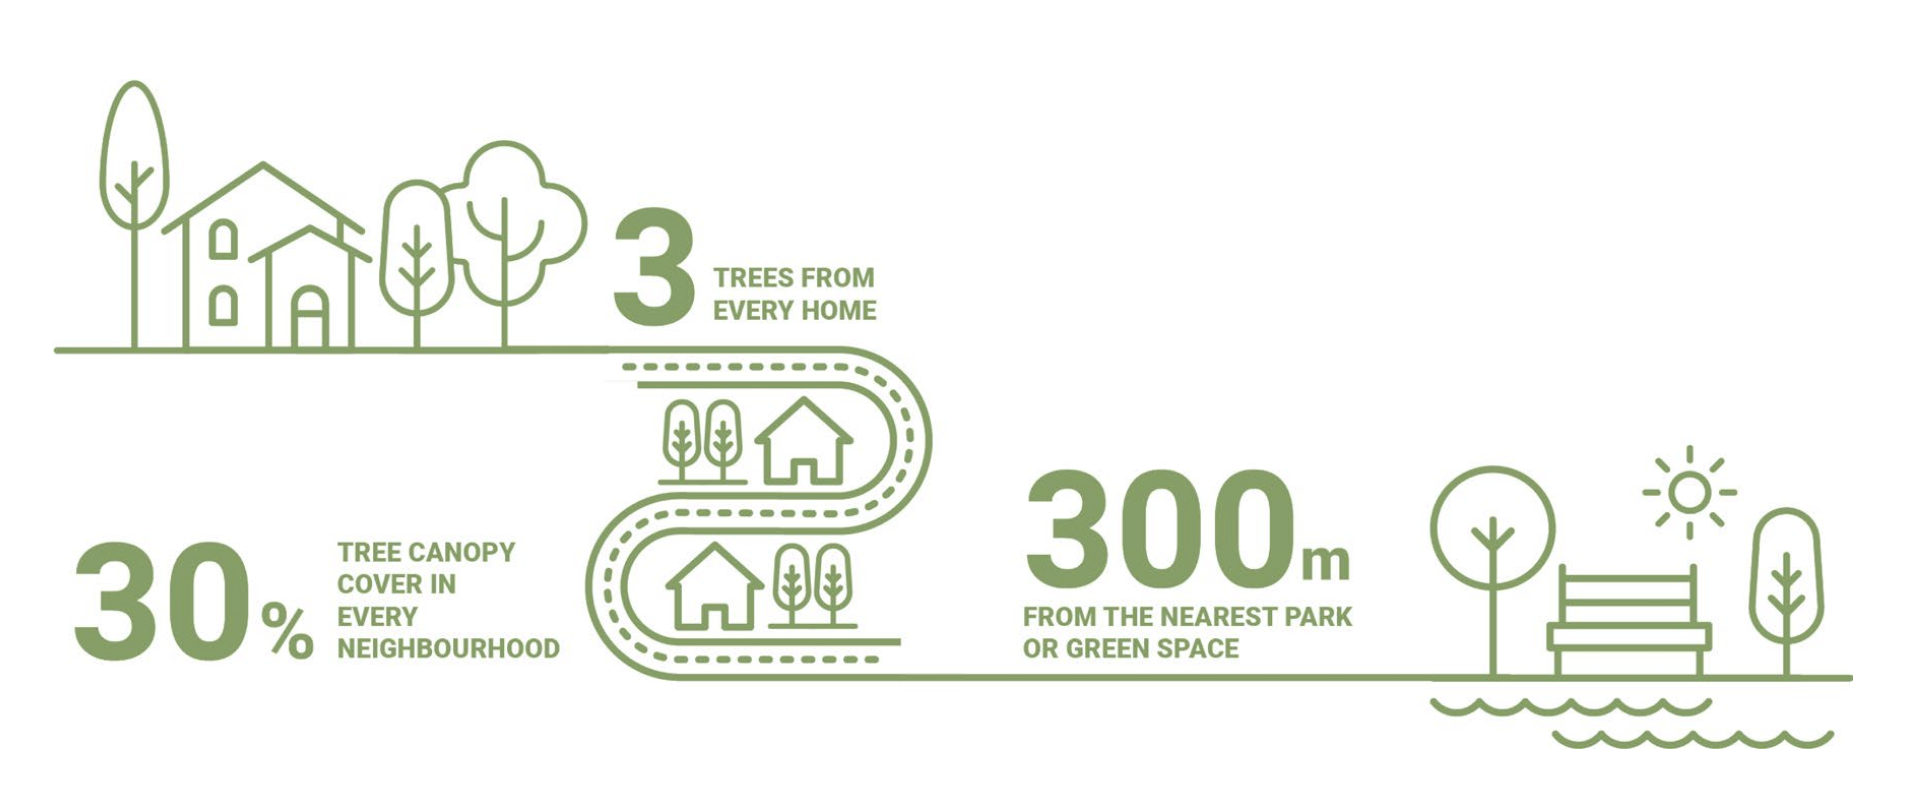
\includegraphics[width=\linewidth]{./figs/schemaUNECE} 

}

\caption{Schema della regola 3-30-300. Da UNECE (2022).}\label{fig:modello330300}
\end{figure}

È interessante notare che queste tre soglie corrispondono a tre modalità distinte di esposizione alla natura: i) vedere la natura, ii) vivere in mezzo al verde e iii) usufruirne a scopo ricreativo e rigenerativo.
Queste soglie non sono arbitrarie, ma si fondano su evidenze empiriche consolidate nella letteratura scientifica.
Ad esempio, il valore del 30\% di verde per ogni quartiere trova riscontro negli studi di Astell-Burt e Feng, che associano a tale soglia maggiori benefici per salute, sonno e salute mentale \citep{feng2017}, mentre i 300 m coincidono con la raccomandazione dell'Ufficio regionale europeo dell'OMS per uno spazio verde di estensione almeno pari a un ettaro \citep{worldhealthorganization2017}.
Ovviamente questa regola è una linea guida ``volontaria'', da applicare con attenzione al contesto locale: tessuti urbani densi o con caratteri storici, congiuntamente a ulteriori fattori culturali, possono rendere difficile e inadeguata l'applicazione letterale delle soglie; la regola tuttavia resta un valido orientamento per una proiezione sostenibile dello sviluppo del tessuto urbano e periurbano.

\section{Agenda urbana e progetto lifeIMAGINE}\label{agenda-urbana-e-progetto-lifeimagine}

=={[}da concordare quali parti inserire{]}==

\section{Obiettivi dello studio}\label{obiettivi-dello-studio}

=={[}altre voci da inserire?{]}==

\chapter{Metodologie}\label{metodologie}

\section{Approccio metodologico generale}\label{approccio-metodologico-generale}

Dal punto di vista metodologico, il piano delle attività è stato condotto sempre in accordo con lo schema concettuale di seguito riportato e già presentato nel 2025 che definisce le principali fasi del lavoro (Fig. \ref{fig:modelloRECSpoleto}).

\begin{figure}

{\centering 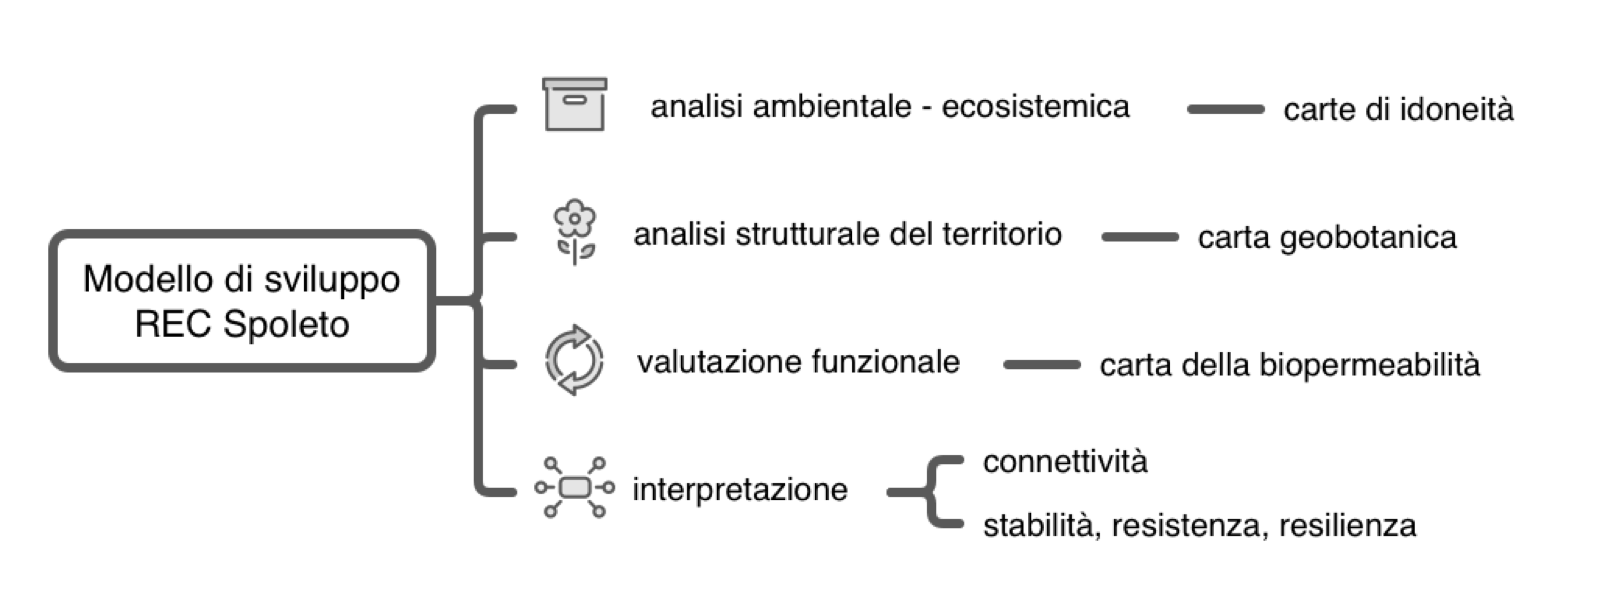
\includegraphics[width=\linewidth]{./figs/RECSpoleto_map03} 

}

\caption{Modello di sviluppo attività.}\label{fig:modelloRECSpoleto}
\end{figure}

In particolare, in continuità con quanto già impostato in precedenza, sono stati sviluppati nuovi elaborati e approfondimenti analitici orientati all'analisi della struttura e connettività ecologica del paesaggio mediante l'applicazione congiunta della Morphological Spatial Pattern Analysis (MSPA) e delle metriche di frammentazione spaziale.
Questa nuova interpretazione tiene conto del passaggio delle precedenti Unità di Paesaggio (UdP) alle nuove Unità Funzionali (UF).
Inoltre, è stata sviluppata una valutazione delle infrastrutture verdi e blu dell'unità urbana, ponendo come base per la verifica preliminare dei criteri di vivibilità e sostenibilità del territorio la regola 3--30--300.

\section{Suddivisione del territorio in unità funzionali}\label{sec-UF}

La definizione di unità territoriali rappresenta un passo fondamentale nella pianificazione territoriale.
Come previsto nell'Art.32 del TITOLO IV delle Norme Tecniche di Attuazione del Piano Regolatore Generale - Parte Strutturale, il Paesaggio Comunale attualmente si articola in 14 Unità di Paesaggio in coerenza con le Unità del Sistema Paesaggistico proposte nell'ambito del PTCP.
L'analisi dell'attuale configurazione delle Unità di Paesaggio (UdP) ha evidenziato un disallineamento con i confini amministrativi consolidati.
In previsione della programmazione del nuovo PRG, si intende superare tale elemento di criticità attraverso l'individuazione di nuove unità di suddivisione del territorio, denominate Unità Funzionali (UF).

\subsection{Approccio metodologico e basi dati}\label{approccio-metodologico-e-basi-dati}

L'approccio metodologico adottato per la definizione delle nuove UF, persegue due obiettivi principali: i) garantire una coerenza amministrativa che si basa sull'allineamento delle UF con i confini esistenti delle frazioni e località e ii) assicurare l'identificazione di ambiti territoriali che presentino caratteristiche paesaggistiche ed ecologico-funzionali il più possibile omogenee.
Tale metodologia ha quindi come obiettivo la continuità dell'organizzazione amministrativa esistente e la suddivisione del territorio in ambiti funzionali che mantengano una propria identità e riconoscibilità.

I supporti informativi di cui si è tenuto conto nel processo di formulazione di questa prima proposta per le UF sono:

\begin{itemize}
\tightlist
\item
  unità di paesaggio
\item
  carta delle macroaree
\item
  carta delle frazioni e località
\item
  modello di elevazione digitale del terreno
\item
  carta CORINE Land Cover (vers. 2018)
\item
  carta geobotanica e uso del suolo aggiornata nell'ambito delle attività per lo sviluppo della rete ecologica comunale
\item
  carta della rete idrografica comunale
\item
  carta dei bacini idrografici
\end{itemize}

Per l'individuazione delle UF come base di partenza è stata utilizzata la carta delle UdP che già identifica ambiti territoriali coerenti e riconoscibili.
Questi ambiti sono stati successivamente estesi o contratti in funzione della carta delle frazioni e località, che ha guidato la rimodellazione dei confini.
Per garantire coerenza amministrativa si è cercato di assegnare ogni frazione a un'unica UF.
Tale assegnazione univoca non è stata tuttavia sempre possibile e pertanto alcuni casi dovranno essere oggetto di ulteriore analisi e approfondimento.

In particolare le frazioni di:

\begin{itemize}
\tightlist
\item
  Bazzano superiore (2)
\item
  Cerqueto (2)
\item
  Morro (2)
\item
  Perchia (2)
\item
  Pompagnano (2)
\item
  Poreta (2)
\item
  San Venanzo (2)
\item
  Sant'Angelo in Mercole (2)
\item
  Silvignano (2)
\end{itemize}

attualmente ricadono in due unità funzionali e nel caso di:

\begin{itemize}
\tightlist
\item
  Eggi (3)
\end{itemize}

si arriva a tre diverse UF.

Per l'assegnazione di ciascuna località a un'unità funzionale è stato adottato il seguente approccio metodologico:

\begin{itemize}
\tightlist
\item
  quando il poligono di una località ricadeva interamente all'interno di una UdP, l'assegnazione alla rispettiva UF è stata diretta.
\item
  nei casi in cui il poligono della località insisteva su più UdP, per l'assegnazione alla relativa UF sono state considerate le sue caratteristiche altitudinali, geobotaniche e di uso del suolo.
\end{itemize}

Infine, per garantire una maggiore coerenza funzionale, sono state considerate anche le macroaree urbane.
Nella collocazione delle località all'interno delle UF si è tenuto conto di questo aspetto, privilegiando l'aggregazione delle porzioni urbanizzate al fine di concentrare in poche unità omogenee i sistemi insediativi più consolidati.

\section{Analisi della struttura e della connettività del paesaggio (MSPA ed Effective Mesh Size)}\label{analisi-della-struttura-e-della-connettivituxe0-del-paesaggio-mspa-ed-effective-mesh-size}

L'indagine sulla struttura e sulla connettività del paesaggio è stata condotta integrando i principi della Morphological Spatial Pattern Analysis (MSPA)\citep{vogt2025} con le metriche di frammentazione spaziale elaborate da \citep{jaeger2000}.
L'analisi è stata eseguita disaggregando le porzioni territoriali in base alle Unità Funzionali del territorio spoletino.
Ciò per confrontare direttamente l'assetto ecologico dei diversi ambiti, ma anche per supportare la pianificazione delle azioni prioritarie necessarie per ciascuna unità con l'obiettivo finale di incrementare la permeabilità della matrice territoriale complessiva e rafforzare l'efficenza della rete ecologica comunale.

È ampiamente consolidato, infatti, come la pianificazione territoriale in ambito urbano e periurbano richieda un approccio integrato, in grado di valorizzare la diversità ambientale a tutela della biodiversità locale.
L'eterogeneità degli habitat costituisce il presupposto fondamentale per garantire condizioni idonee alle specie autoctone e preservare la continuità dei corridoi ecologici \citep{battisti2004, vilenica2020}.

In questo contesto, la metodologia MSPA offre il vantaggio di sintetizzare la complessità del mosaico paesaggistico in un modello concettuale articolato su due componenti chiave:

\begin{itemize}
\tightlist
\item
  Sistema degli Habitat: che rappresenta il nucleo ad alto valore ecologico e conservazionistico, derivante dall'integrazione tra le diverse categorie geobotaniche e coperture del suolo. In altri termini, questo sistema costituisce l'insieme dei tasselli ad elevata idoneità in grado di supportare le funzioni vitali delle specie target e favorirne gli spostamenti.
\item
  Matrice di Background: che comprende le porzioni di territorio con finalità produttive a prevalente impronta antropica, o a minore naturalità, caratterizzate da condizioni ambientali generalmente subottimali. Essa agisce da spazio di transizione e tendenzialmente presenta una limitata capacità di supporto diretto per la fauna locale.
\end{itemize}

L'applicazione di questo schema concettuale permette di contestualizzare le metriche morfologiche MSPA (Core, Bridge, Islet, Edge, ecc.) all'interno di un quadro interpretativo coerente e aiutare i processi della pianificazione indirizzandoli verso l'individuazione delle aree prioritarie per la conservazione e quelle mirate alla deframmentazione e potenziamento della connettività ecologica.

Per questa sintesi basata sulle Unità Funzionali spoletine, le categorie MSPA sono state aggregate in 7 macro-categorie morfologiche fondamentali:

\begin{enumerate}
\def\labelenumi{\arabic{enumi}.}
\tightlist
\item
  Core: le aree interne e contigue della matrice naturale, con ruolo primario di serbatoio di biodiversità e habitat biologico principale.
\item
  Islet: piccoli frammenti isolati e discontinui di habitat naturale che non raggiungono la dimensione minima di area core.
\item
  Perforation: i margini e i varchi interni alle aree \emph{Core}, generati da discontinuità della copertura vegetale.
\item
  Edge: la fascia di transizione e margine esterno che delimita le aree \emph{Core} verso il background o la matrice antropizzata.
\item
  Loop: corridoi o elementi lineari che collegano un'area \emph{Core} a se stessa (corridoi interni o di auto-connessione), incluse le variazioni di margine e perforazione (\emph{Loop in Edge}, \emph{Loop in Perforation}).
\item
  Bridge: elementi lineari e corridoi strutturali che collegano due o più aree \emph{Core} distinte, rappresentando la spina dorsale della connettività ecologica funzionale.
\item
  Branch: corridoi lineari o bracci che dipartono da un'area \emph{Core} ma terminano a fondo cieco, senza connettersi ad altri elementi. {[}Queste porzione evidenziano connessioni interrotte che se opportunamente riconosciute e valorizzate potrebbero fornire con interventi minimi un grado di connettività molto superiore.{]}
\end{enumerate}

Per ciascuna Unità Funzionale e per ciascuna delle 7 macro-categorie MSPA sono state calcolate tre metriche chiave:

\begin{enumerate}
\def\labelenumi{\arabic{enumi}.}
\tightlist
\item
  Area Totale: espressa in ettari (ha), rappresenta l'estensione complessiva occupata da ciascuna tipologia MSPA all'interno dell'unità funzionale.
\item
  Numero di Patches: indica il conteggio totale di poligoni/frammenti distinti appartenenti a ciascuna categoria. Questo valore è rilevante poiché il rapporto tra \emph{Area Totale} e \emph{Numero di Patches} esprime la dimensione media degli elementi del mosaico paesaggistico.
\item
  Effective Mesh Size: definita secondo la formulazione di \citep{jaeger2000}, calcola la dimensione utile di maglia ed è un indicatore di connettività e integrità del paesaggio:
\end{enumerate}

\[S_{eff} = \frac{\sum_{i=1}^{n} A_i^2}{A_{tot\_unita}}\]

Dove:

\begin{itemize}
\tightlist
\item
  \(A_i\) è la superficie del singolo poligono (patch) appartenente a una determinata classe MSPA.
\item
  \(A_{tot\_unita}\) è la superficie complessiva dell'Unità Funzionale di riferimento.
\end{itemize}

Per l'interpretazione del significato ecologico dell'indice di Effective Mesh Size - \(S_{eff}\) occorre tenere presente che a parità di superficie totale occupata da una categoria, un valore di Effective Mesh Size (\(S_{eff}\)) più elevato indica una maggiore continuità spaziale e aggregazione dei tasselli (bassa frammentazione).
Al contrario, un valore di \(S_{eff}\) molto basso riflette una forte polverizzazione dell'habitat in frammenti di ridotte dimensioni, aumentando la probabilità di isolamento ecologico.

\section{Analisi del sistema verde e blu urbano}\label{analisi-del-sistema-verde-e-blu-urbano}

L'indagine ha preso in esame la composizione e l'organizzazione spaziale dei sistemi verdi e blu che caratterizzano il territorio comunale di Spoleto, utilizzando come base conoscitiva il tematismo del verde pubblico e privato, comprensivo delle infrastrutture blu.

Attraverso questo studio, finalizzato a descrivere estensione, distribuzione, livello di continuità e relazioni funzionali e spaziali tra le diverse componenti, vengono definiti gli elementi strutturali necessari per condurre una valutazione preliminare del grado di conformità del contesto urbano rispetto ai parametri della regola 3--30--300.

Per approfondire la configurazione, il ruolo funzionale e le caratteristiche generali di tali componenti, è stata eseguita un'analisi di paesaggio basata sugli indicatori del pacchetto landscapemetrics (BIBLIO).

Tale libreria riprende le metriche storicamente implementate in FRAGSTAT {[}@mcgarigalFragstatHelp2015{]} e ne estende le potenzialità per un utilizzo multipiattaforma. Nell'ambito di questa relazione sono state considerate le seguenti metriche, risultate particolarmente efficaci per una descrizione analitica dell'assetto generale dell'area.

Elenco delle variabili landscapemetrics esaminate:

\begin{itemize}
\tightlist
\item
  LPI (Largest Patch Index): Misura la percentuale del paesaggio occupata dalla patch più estesa appartenente a una determinata classe. È un indicatore di dominanza e continuità spaziale. Nel caso delle infrastrutture verdi, un LPI elevato suggerisce la presenza di un grande nucleo verde capace di sostenere funzioni ecologiche rilevanti.
\item
  Superficie Mediana (Median Patch Area): Rappresenta la dimensione della patch che divide la distribuzione in due metà: il 50\% delle patch è più piccolo e il 50\% è più grande. Fornisce una misura robusta della dimensione tipica delle patch, meno influenzata dai valori estremi rispetto alla superficie media.
\item
  PD (Patch Density): Numero di patch presenti per unità di superficie (solitamente per 100 ha). È una delle metriche più utilizzate per valutare il livello di frammentazione del paesaggio. Va sempre interpretata insieme alle dimensioni delle patch.
\item
  AI (Aggregation Index): Misura il grado con cui le celle o le patch della stessa classe risultano spazialmente aggregate. Descrive quanto gli elementi della stessa classe tendano a formare blocchi continui anziché essere distribuiti in modo frammentato.
\item
  COHESION (Patch Cohesion Index): Misura il grado di connessione fisica delle patch appartenenti a una stessa classe. È particolarmente utile per comprendere se gli habitat o le infrastrutture verdi mantengono una continuità funzionale su scala territoriale. Nel contesto urbano, valori molto elevati possono indicare che numerosi elementi verdi, pur frammentati, risultano comunque parte di una rete spazialmente connessa.
\item
  CONTAG (Contagion Index): Misura il grado di aggregazione complessiva delle classi presenti nel paesaggio considerando tutte le tipologie di copertura. Descrive la configurazione generale del paesaggio e il livello di mescolamento tra le diverse classi.
\item
  CLUMPY (Clumpiness Index): Valuta quanto una classe sia aggregata rispetto a una distribuzione casuale. È una misura molto efficace per confrontare il grado di aggregazione tra classi con abbondanze molto differenti.
\item
  CORE (Core Area): Misura la superficie situata oltre una determinata distanza dal margine della patch (edge depth). È una metrica fondamentale per valutare la qualità ecologica delle aree verdi, poiché molte specie e funzioni ecosistemiche richiedono habitat interni protetti dalle perturbazioni provenienti dall'esterno.
\item
  ENN (Euclidean Nearest Neighbor Distance): Misura la distanza lineare tra una patch e la patch più vicina appartenente alla stessa classe. È una delle metriche più utilizzate per valutare la connettività potenziale. Non misura l'effettiva connessione ecologica, ma la vicinanza spaziale tra elementi dello stesso tipo.
\end{itemize}

=={[}da integrare: criteri adottati per la verifica preliminare della regola 3--30--300 (aree di verde pubblico di estensione prossima a 1 ha, buffer di 300 m){]}==

\section{Approccio all'analisi del territorio con Marxan}\label{approccio-allanalisi-del-territorio-con-marxan}

=={[}prima bozza in fase di completamento{]}==

\section{Citizen science e sondaggio}\label{citizen-science-e-sondaggio}

=={[}da redigere: impianto metodologico della campagna di citizen science e del sondaggio{]}==

\chapter{Risultati}\label{risultati}

\section{Quadro conoscitivo di base}\label{quadro-conoscitivo-di-base}

\subsection{Schede descrittive delle Unità Funzionali}\label{schede-descrittive-delle-unituxe0-funzionali}

L'applicazione della metodologia descritta in sezione \ref{sec-UF} ha permesso di ridefinire l'assetto del territorio comunale, superando il disallineamento strutturale tra le precedenti Unità di Paesaggio e i confini amministrativi consolidati.
Il processo di integrazione dei supporti informativi ha condotto all'individuazione della nuova configurazione in Unità Funzionali (UF).
Di seguito vengono presentati i risultati dell'elaborazione per ciascuna Unità Funzionale, evidenziandone le sue caratteristiche principali.

\subsubsection{UF Alto collinare montana dell'Appennino (19)}\label{uf-alto-collinare-montana-dellappennino-19}

\begin{quote}
Superficie: 131.6 km\^{}2

Range altitudinale: 270 - 1328 m s.l.m.

Quota mediana: 729 m s.l.m.
\end{quote}

\begin{figure}

{\centering 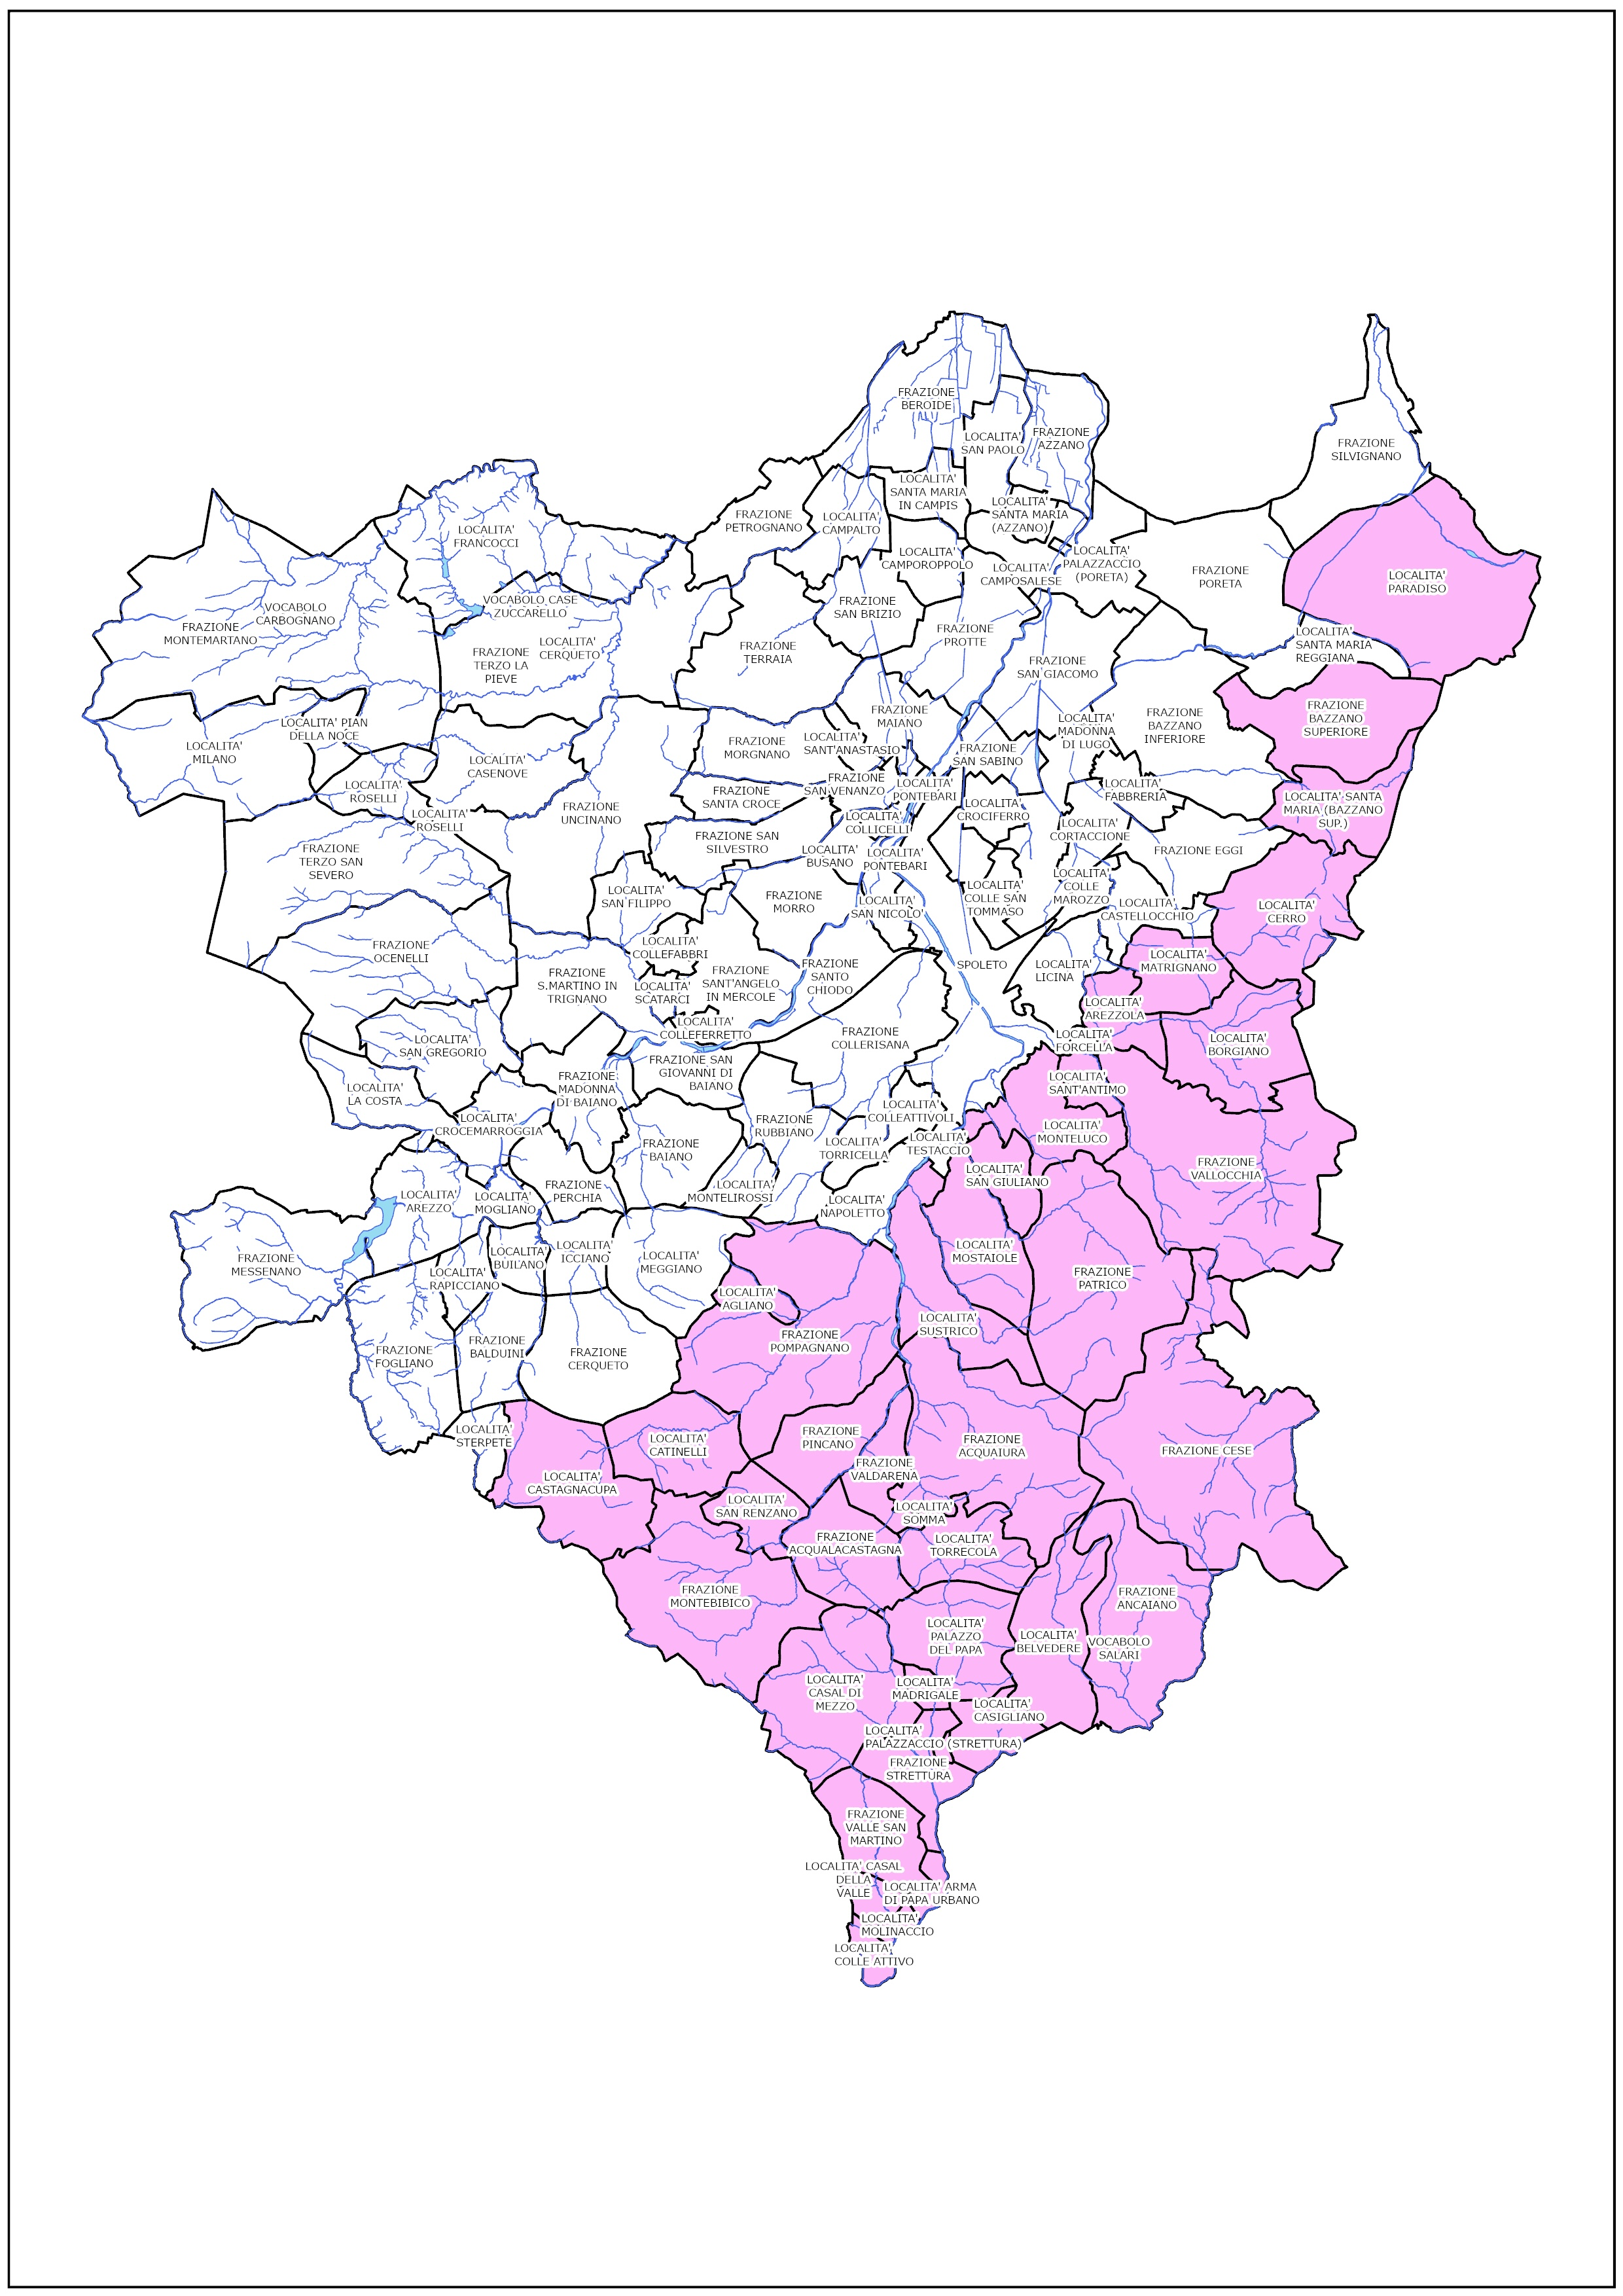
\includegraphics[width=\linewidth]{./figs/stampeCorrado/UFAppennino} 

}

\caption{Unità Funzionale Alto collinare montana dell'Appennino. Elaborazione cartografica C. Arcangeli.}\label{fig:UFAppennino}
\end{figure}

Questa unità funzionale potenzialmente raccoglie 16 frazioni e 3 località.

\begin{verbatim}
FRAZIONE ACQUAIURA
FRAZIONE ACQUALACASTAGNA
FRAZIONE ANCAIANO
FRAZIONE BAZZANO SUPERIORE (BAZZANO SUPERIORE, SANTA MARIA)
FRAZIONE CERQUETO (CATINELLI, CASTAGNACUPA)
FRAZIONE CESE
FRAZIONE EGGI (MATRIGNANO, CERRO)
FRAZIONE MONTEBIBICO
FRAZIONE PATRICO
FRAZIONE PINCANO
FRAZIONE POMPAGNANO (POMPAGNANO, AGLIANO)
FRAZIONE SILVIGNANO
FRAZIONE STRETTURA
FRAZIONE VALDARENA
FRAZIONE VALLE SAN MARTINO
FRAZIONE VALLOCCHIA
LOCALITA' MONTELUCO
LOCALITA' SAN GIULIANO
LOCALITA' SANT'ANTIMO
\end{verbatim}

\subsubsection{UF Alto collinare montana dei Monti Martani (3)}\label{uf-alto-collinare-montana-dei-monti-martani-3}

\begin{quote}
Superficie: 41.6 km\^{}2

Range altitudinale: 345 - 1103 m s.l.m.

Quota mediana: 608 m s.l.m.
\end{quote}

\begin{figure}

{\centering 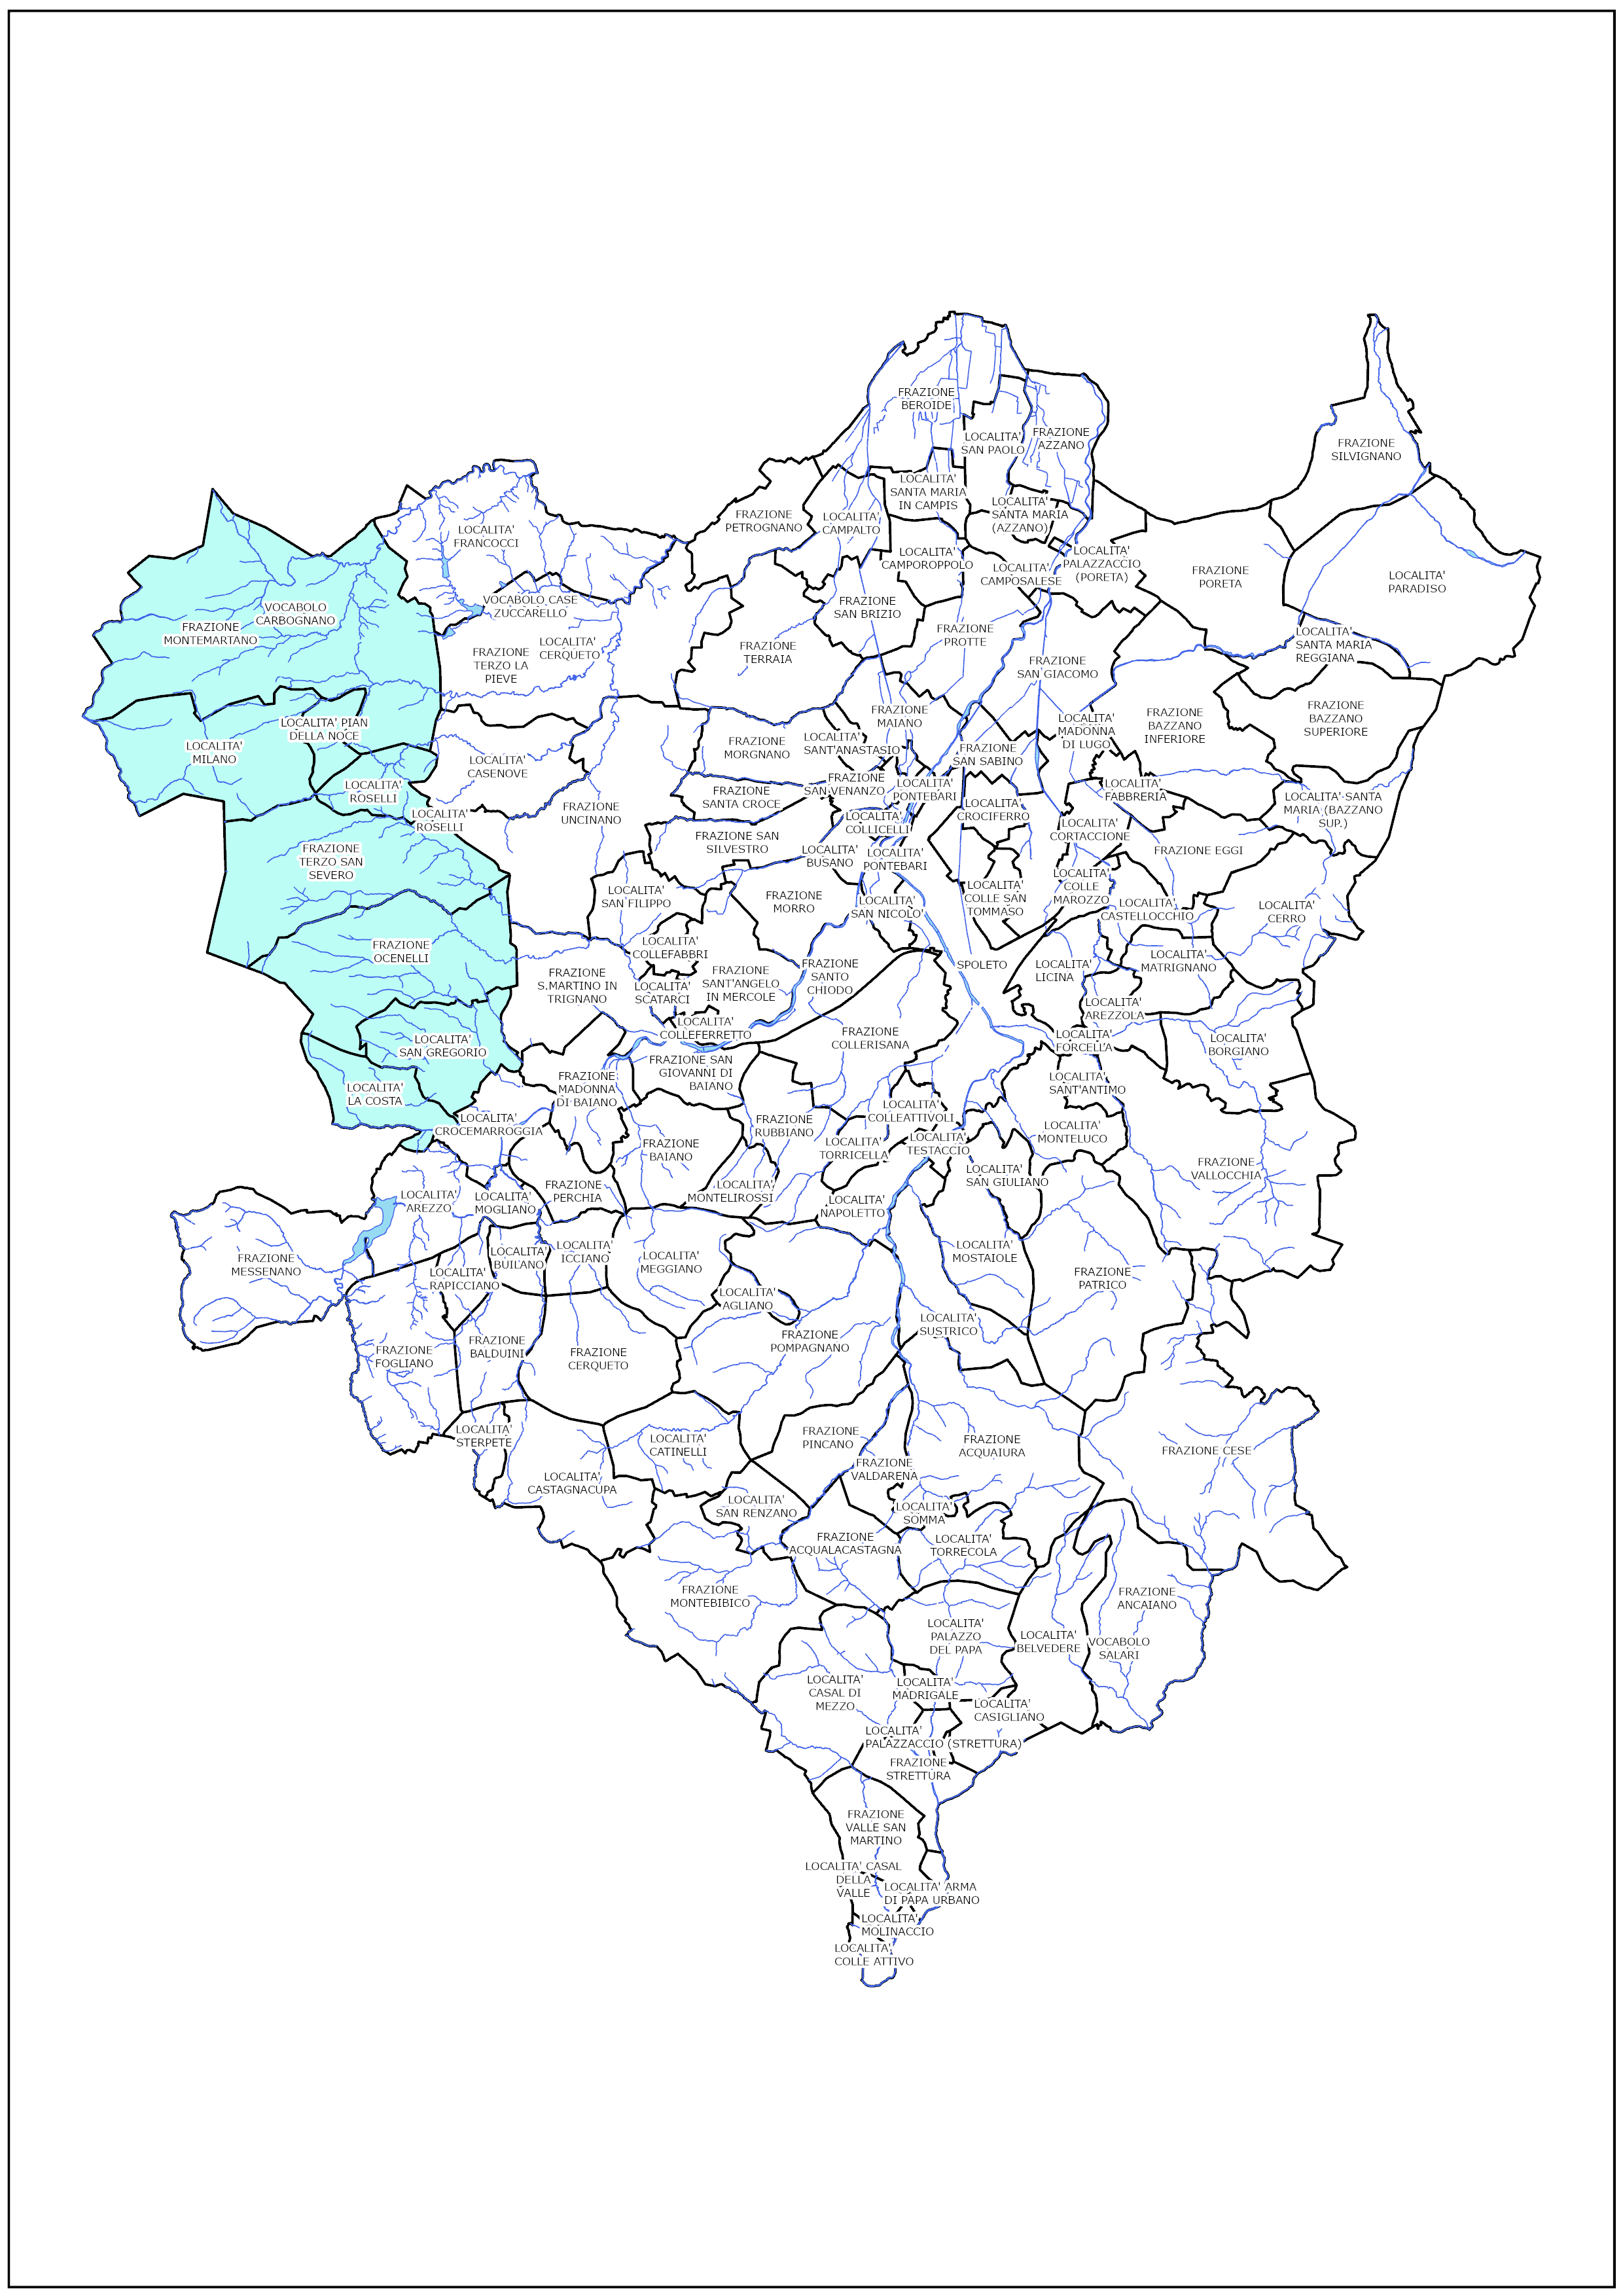
\includegraphics[width=\linewidth]{./figs/stampeCorrado/UFmontanaMMartani} 

}

\caption{Unità Funzionale Alto collinare montana dei Monti Martani. Elaborazione cartografica C. Arcangeli.}\label{fig:UFMMartani}
\end{figure}

Questa unità funzionale potenzialmente si compone di 3 frazioni.

\begin{verbatim}
FRAZIONE MONTEMARTANO
FRAZIONE OCENELLI
FRAZIONE TERZO SAN SEVERO
\end{verbatim}

\subsubsection{UF Collinare di Meggiano (12)}\label{uf-collinare-di-meggiano-12}

\begin{quote}
Superficie: 26.8 km\^{}2

Range altitudinale: 340 - 876 m s.l.m.

Quota mediana: 541 m s.l.m.
\end{quote}

\begin{figure}

{\centering 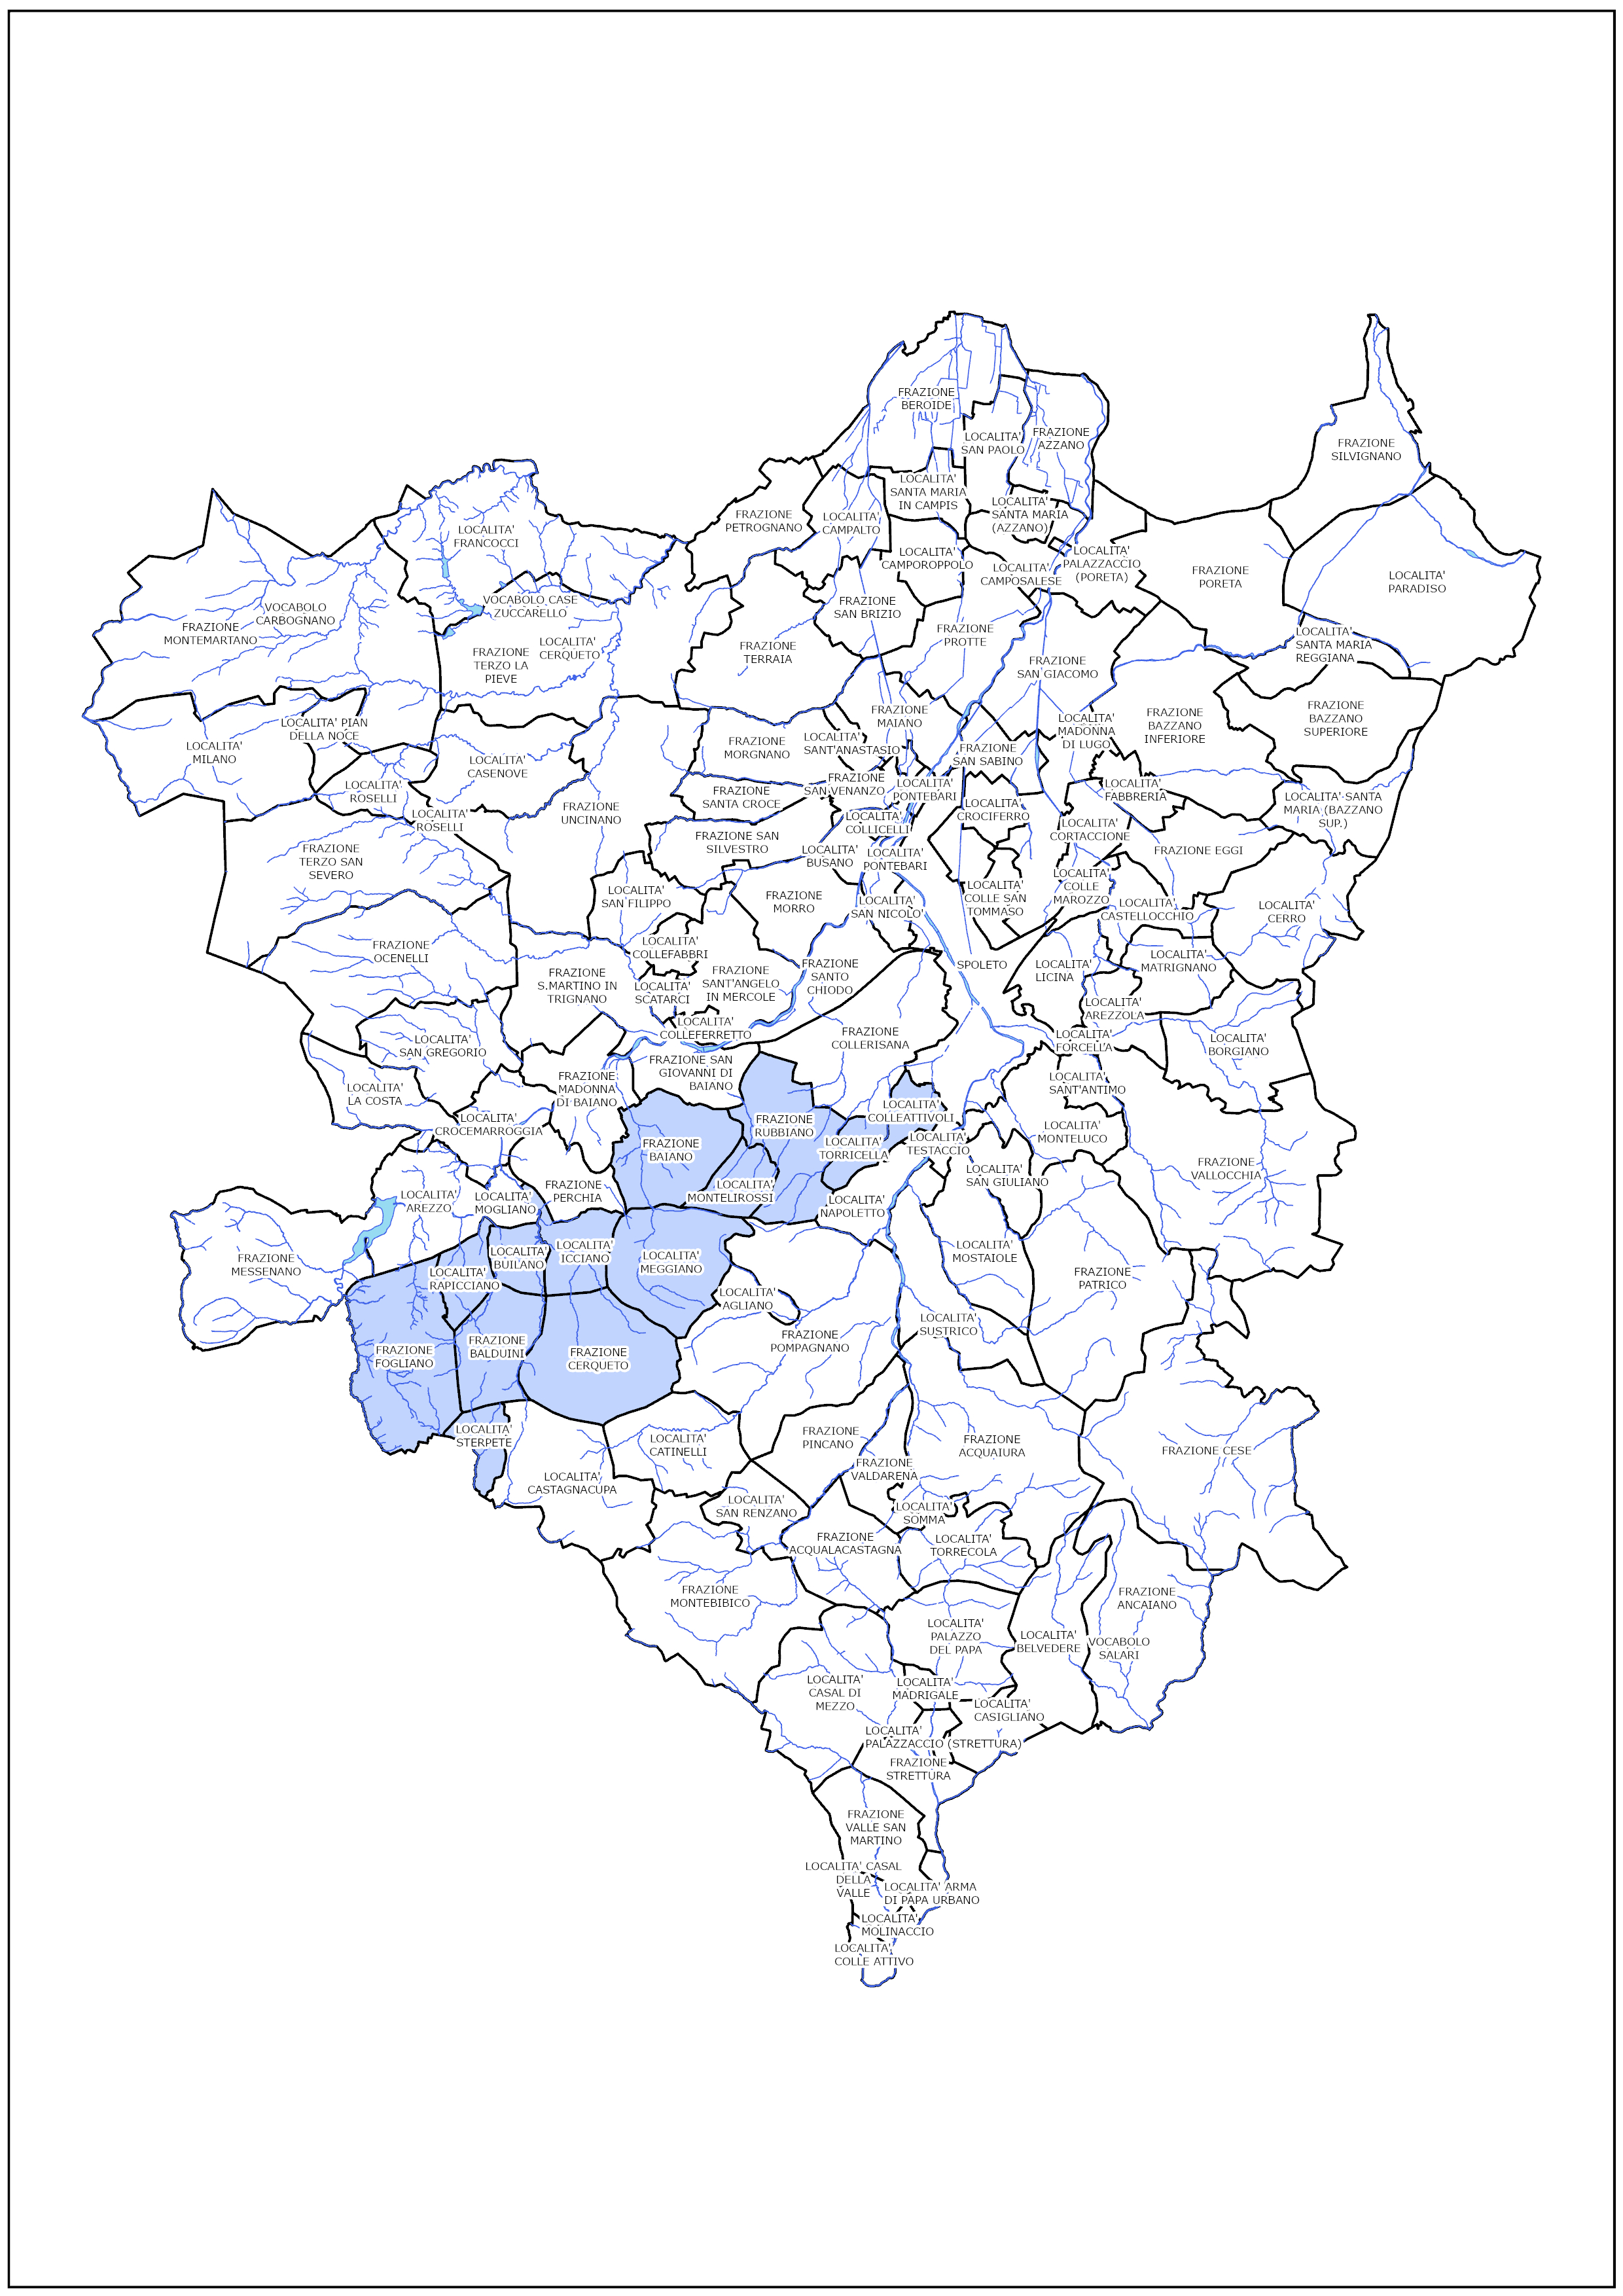
\includegraphics[width=\linewidth]{./figs/stampeCorrado/UFCollinareMeggiano} 

}

\caption{Unità Funzionale Collinare di Meggiano. Elaborazione cartografica C. Arcangeli.}\label{fig:UFCollinareMeggiano}
\end{figure}

Questa unità funzionale potenzialmente raccoglie 8 frazioni e 2 località.

\begin{verbatim}
FRAZIONE BAIANO
FRAZIONE BALDUINI
FRAZIONE CERQUETO (CERQUETO)
FRAZIONE FOGLIANO
FRAZIONE MESSENANO
FRAZIONE PERCHIA (ICCIANO)
FRAZIONE POMPAGNANO (MEGGIANO)
FRAZIONE RUBBIANO
LOCALITA' COLLEATTIVOLI
LOCALITA' TORRICELLA
\end{verbatim}

\subsubsection{UF Collinare - fascia olivata (8)}\label{uf-collinare---fascia-olivata-8}

\begin{quote}
Superficie: 24.4 km\^{}2

Range altitudinale: 247 - 1000 m s.l.m.

Quota mediana: 362 m s.l.m.
\end{quote}

\begin{figure}

{\centering 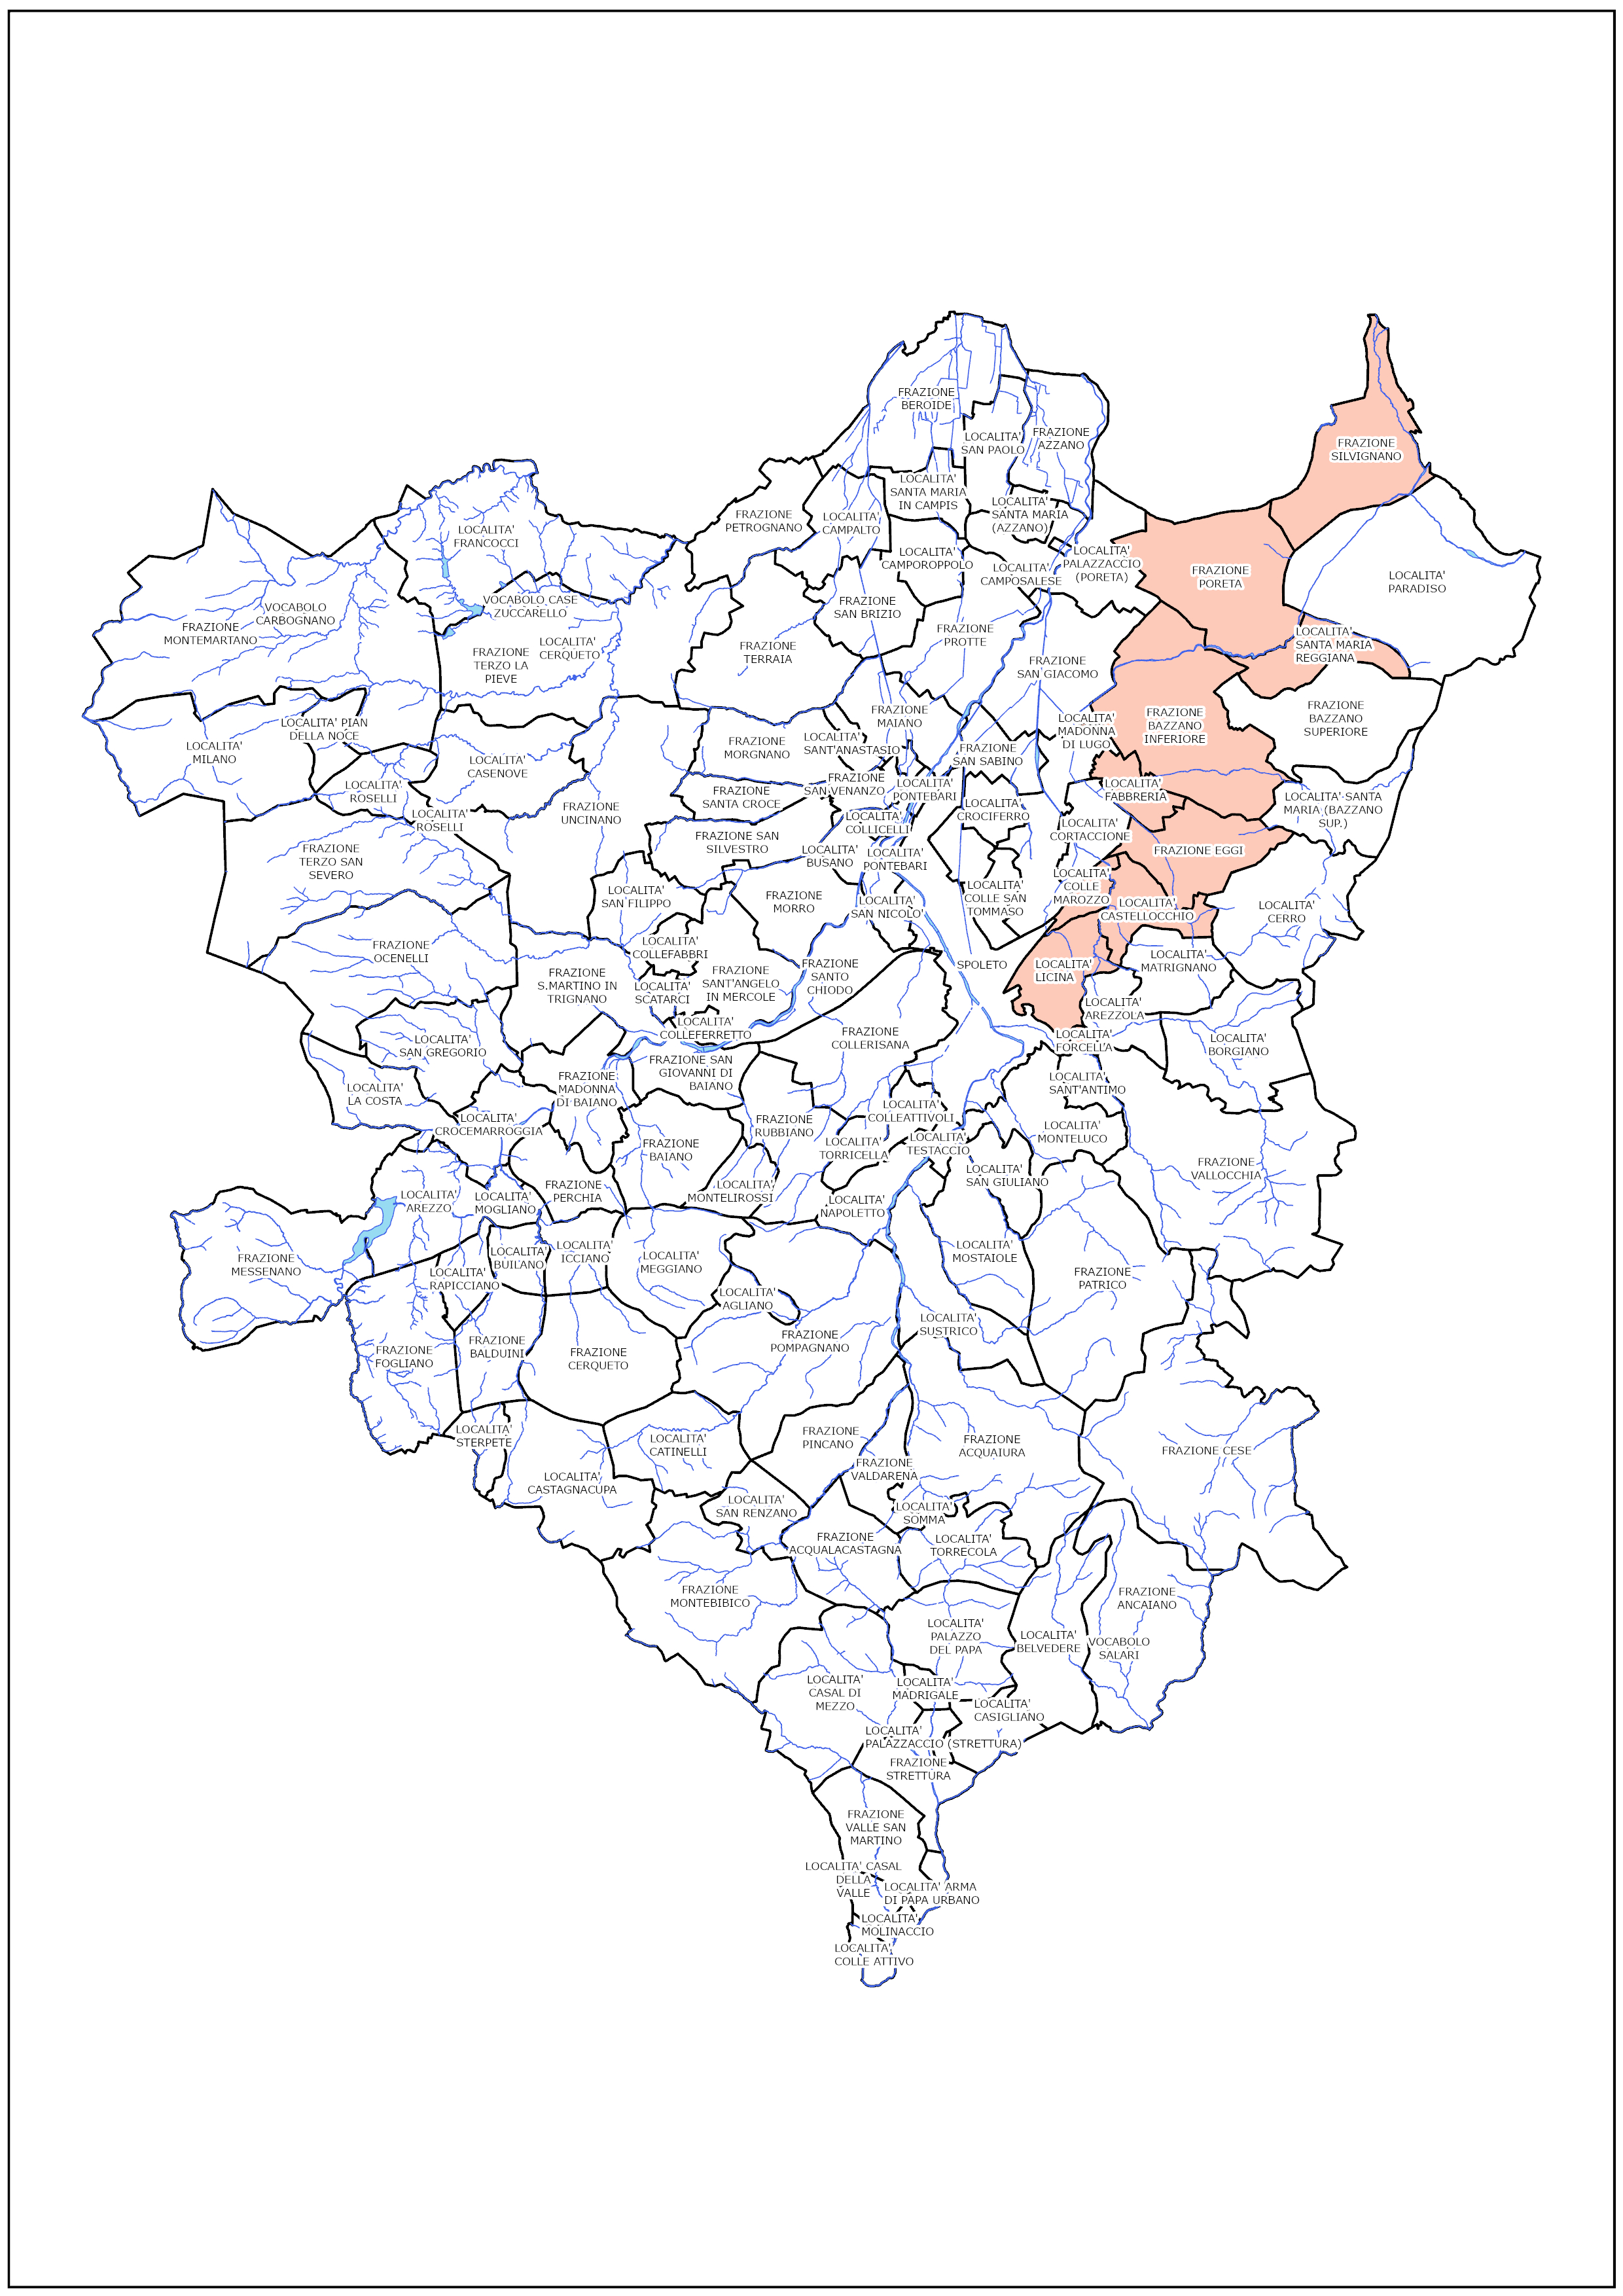
\includegraphics[width=\linewidth]{./figs/stampeCorrado/UFCollinareOlivata} 

}

\caption{Unità Funzionale Collinare - fascia olivata. Elaborazione cartografica C. Arcangeli.}\label{fig:UFCollinareOlivata}
\end{figure}

Questa unità funzionale potenzialmente raccoglie 5 frazioni e 2 località.

\begin{verbatim}
FRAZIONE BAZZANO INFERIORE
FRAZIONE BAZZANO SUPERIORE (SANTA MARIA REGGIANA)
FRAZIONE EGGI (FABBRERIA, EGGI, CASTELLOCCHIO, COLLE MAROZZO)
FRAZIONE PORETA (PORETA)
FRAZIONE SILVIGNANO
LOCALITA' FORCELLA
LOCALITA' LICINA
\end{verbatim}

\subsubsection{UF Collinare dei Monti Martani (10)}\label{uf-collinare-dei-monti-martani-10}

\begin{quote}
Superficie: 43.7 km\^{}2

Range altitudinale: 238 - 527 m s.l.m.

Quota mediana: 337 m s.l.m.
\end{quote}

\begin{figure}

{\centering 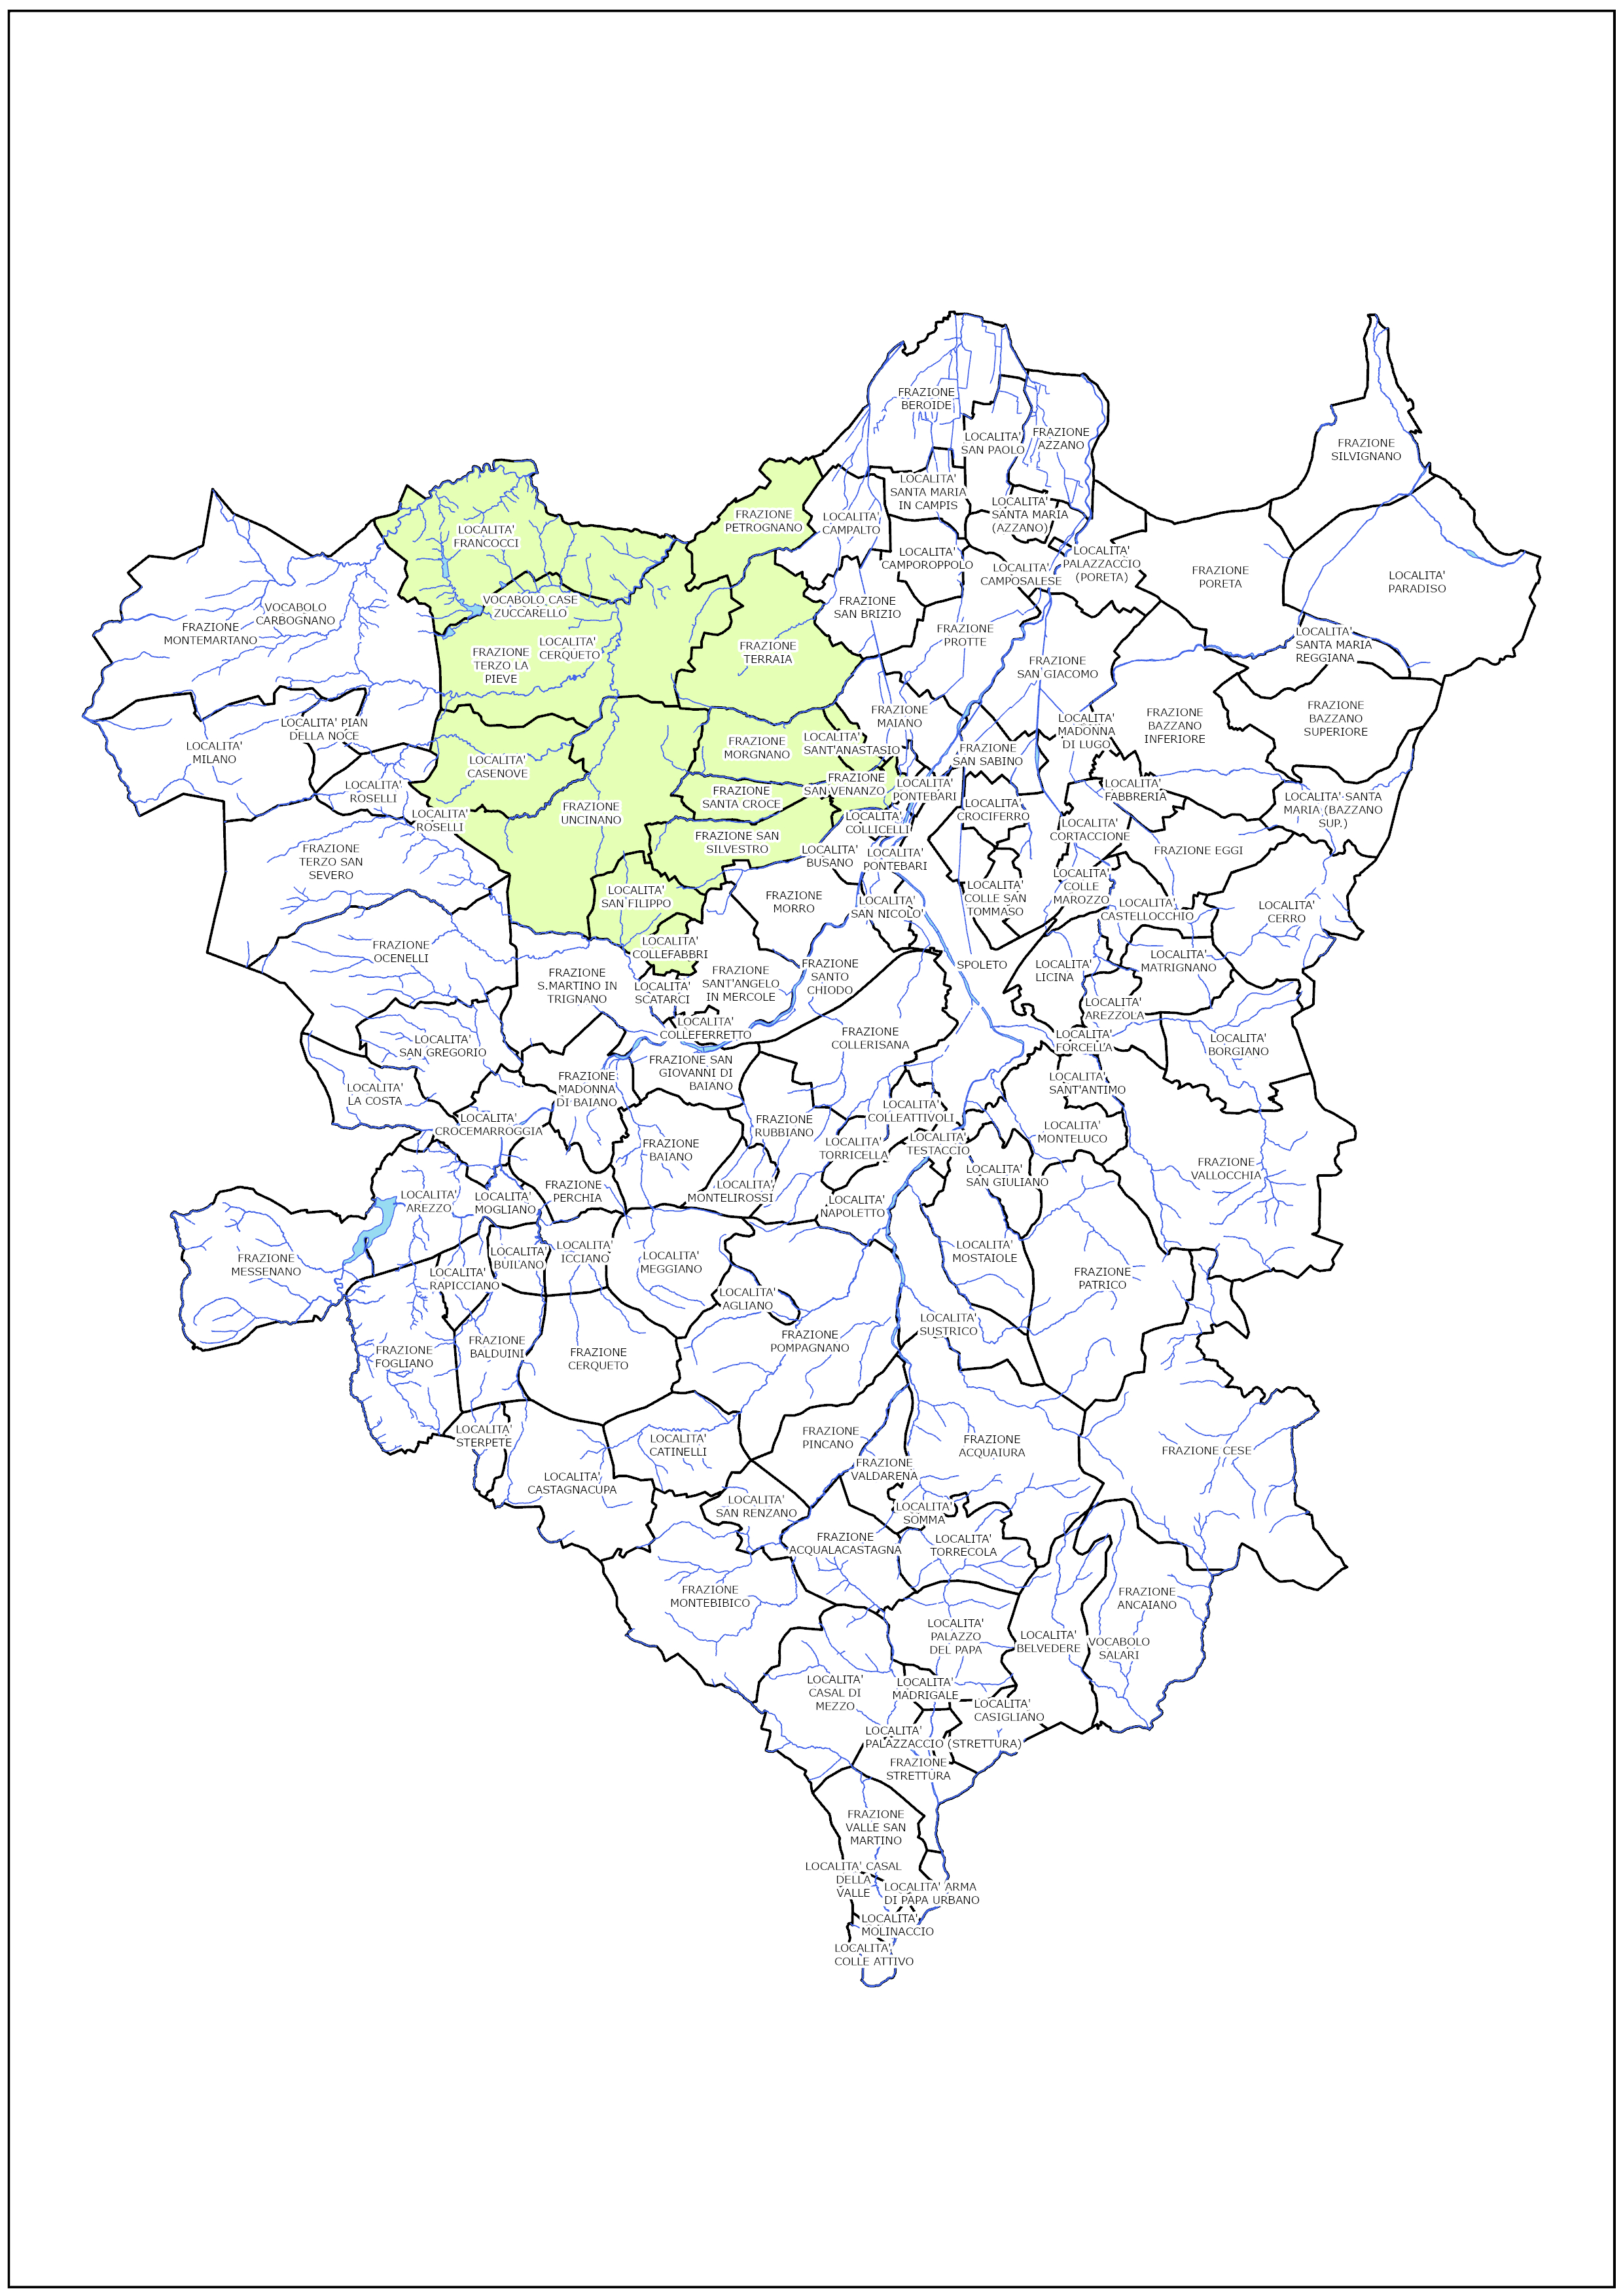
\includegraphics[width=\linewidth]{./figs/stampeCorrado/UFCollinareMMartani} 

}

\caption{Unità Funzionale Collinare dei Monti Martani. Elaborazione cartografica C. Arcangeli.}\label{fig:UFCollinareMMartani}
\end{figure}

Questa unità funzionale potenzialmente si compone di 10 frazioni.

\begin{verbatim}
FRAZIONE MORGNANO
FRAZIONE PETROGNANO
FRAZIONE SAN SILVESTRO
FRAZIONE SAN VENANZO (SANT'ANASTASIO, SAN VENANZO)
FRAZIONE SANT'ANGELO IN MERCOLE (COLLEFABBRI, SAN FILIPPO)
FRAZIONE SANTA CROCE
FRAZIONE TERRAIA
FRAZIONE TERZO LA PIEVE
FRAZIONE TERZO SAN SEVERO
FRAZIONE UNCINANO
\end{verbatim}

\subsubsection{UF di pianura e di Valle del T. Marroggia (15)}\label{uf-di-pianura-e-di-valle-del-t.-marroggia-15}

\begin{quote}
Superficie: 58.6 km\^{}2

Range altitudinale: 222 - 752 m s.l.m.

Quota mediana: 275 m s.l.m.
\end{quote}

\begin{figure}

{\centering 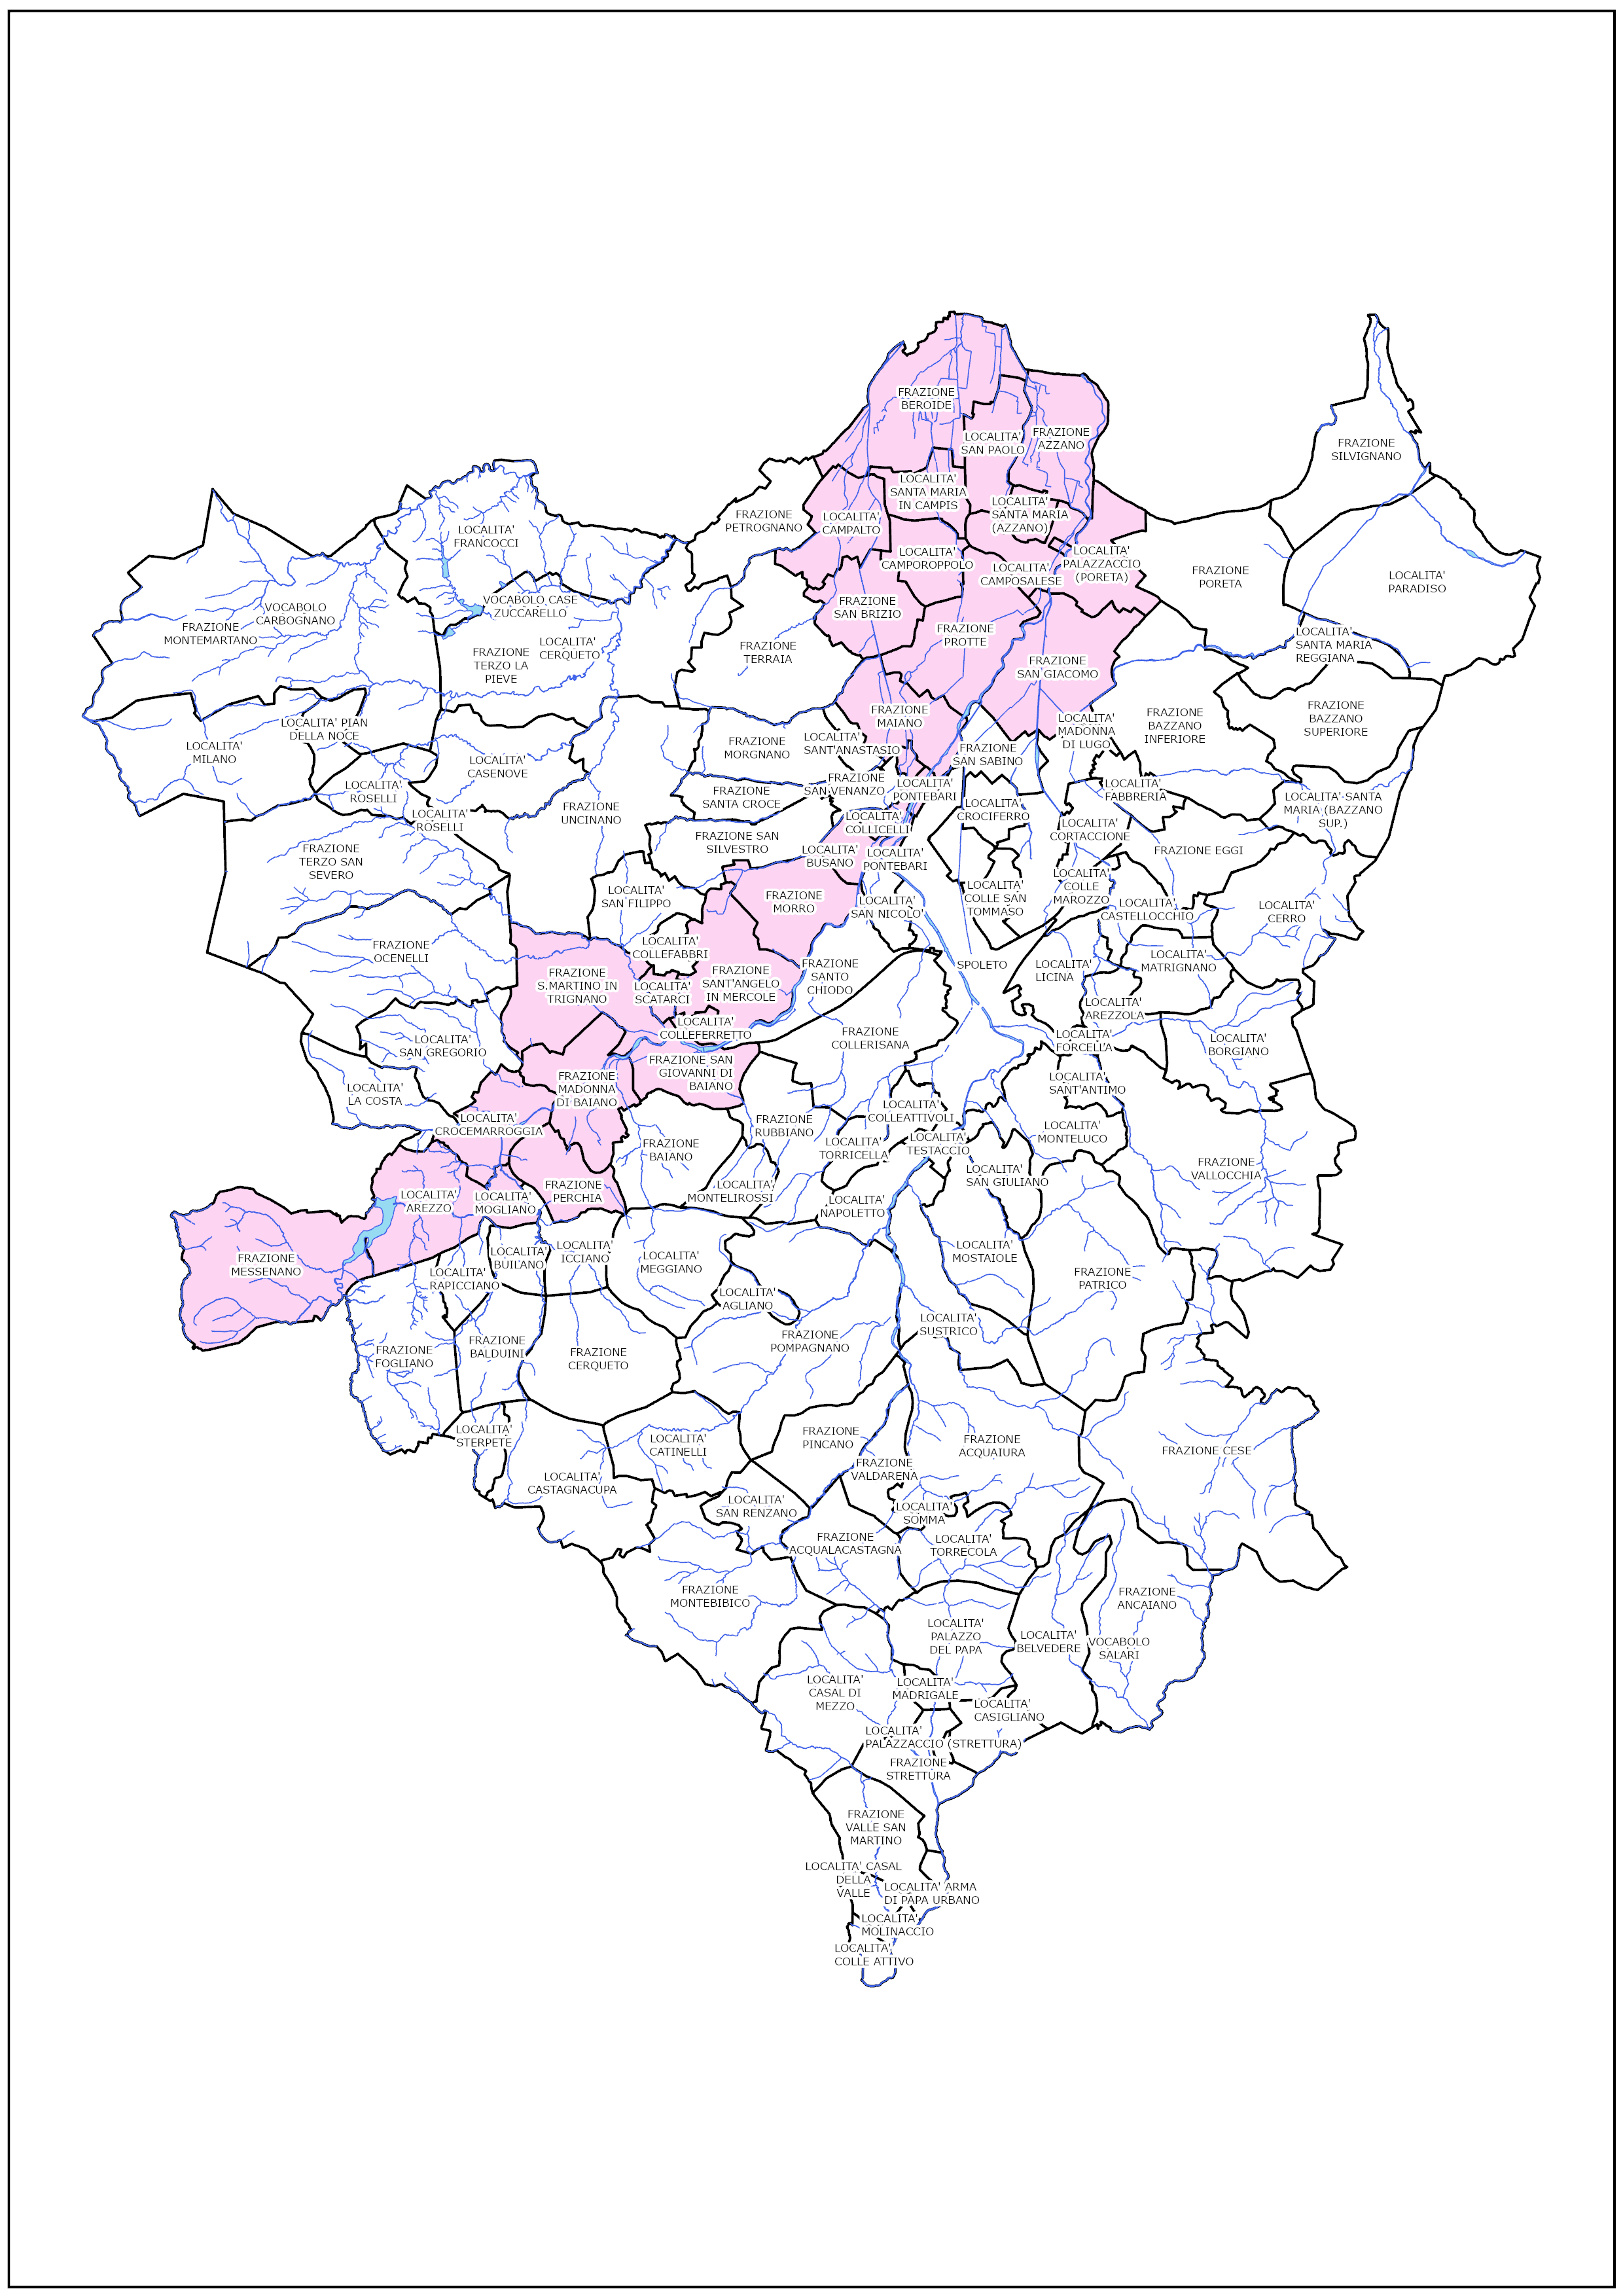
\includegraphics[width=\linewidth]{./figs/stampeCorrado/UFValle} 

}

\caption{Unità Funzionale di pianura e di Valle del T. Marroggia. Elaborazione cartografica C. Arcangeli.}\label{fig:UFValle}
\end{figure}

Questa unità funzionale potenzialmente si compone di 15 frazioni.

\begin{verbatim}
FRAZIONE AZZANO
FRAZIONE BEROIDE
FRAZIONE MADONNA DI BAIANO
FRAZIONE MAIANO
FRAZIONE MESSENANO
FRAZIONE MORRO (BUSANO, MORRO)
FRAZIONE PERCHIA (PERCHIA, MOGLIANO, CROCEMARROGGIA)
FRAZIONE PORETA (PALAZZACCIO)
FRAZIONE PROTTE
FRAZIONE S.MARTINO IN TRIGNANO
FRAZIONE SAN BRIZIO
FRAZIONE SAN GIACOMO
FRAZIONE SAN GIOVANNI DI BAIANO
FRAZIONE SAN VENANZO (MALFONDO, PONTEBARI, COLLICELLI)
FRAZIONE SANT'ANGELO IN MERCOLE (SCATARCI, COLLEFERRETTO, SANT'ANGELO IN MERCOLE)
\end{verbatim}

\subsubsection{Urbana (6)}\label{urbana-6}

\begin{quote}
Superficie: 23 km\^{}2

Range altitudinale: 245 - 651 m s.l.m.

Quota mediana: 300 m s.l.m.
\end{quote}

\begin{figure}

{\centering 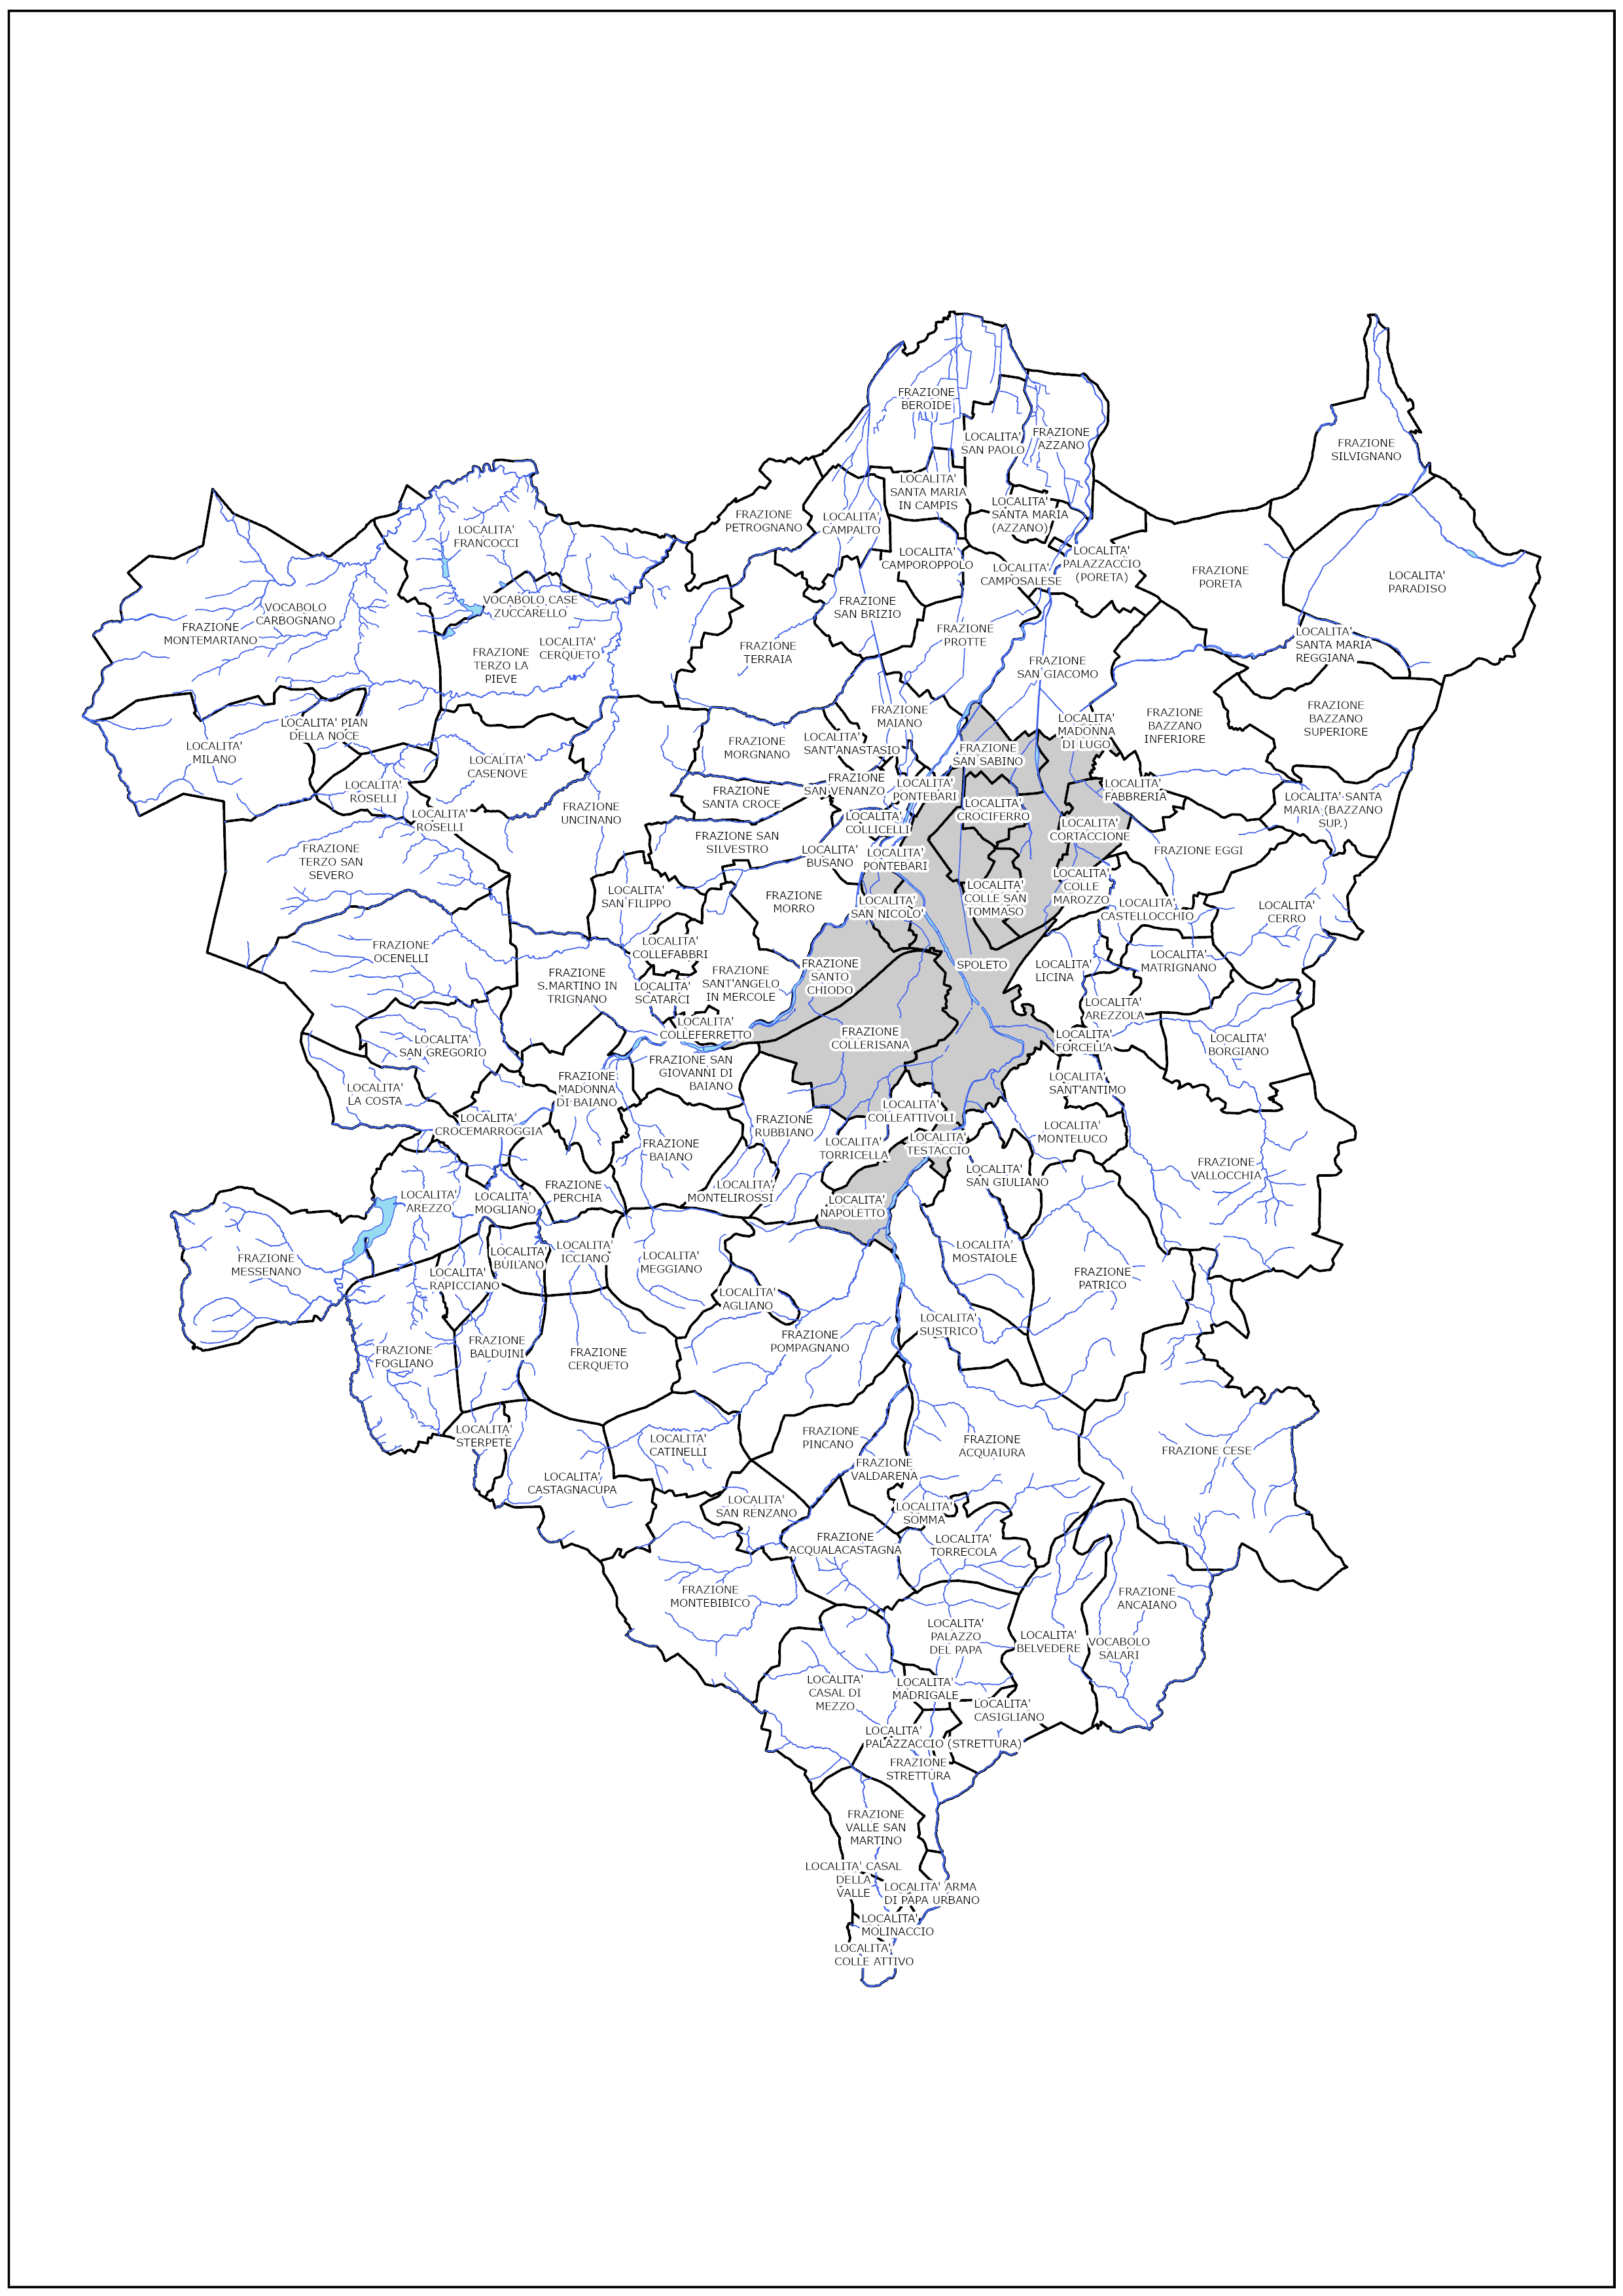
\includegraphics[width=\linewidth]{./figs/stampeCorrado/UFUrbana} 

}

\caption{Unità Funzionale Urbana. Elaborazione cartografica C. Arcangeli.}\label{fig:UFUrbana}
\end{figure}

Questa unità funzionale potenzialmente si compone di 5 frazioni, 2 località e il nucleo della città di Spoleto.

\begin{verbatim}
FRAZIONE COLLERISANA
FRAZIONE EGGI (CORTACCIONE)
FRAZIONE MORRO (SAN NICOLO')
FRAZIONE SAN SABINO
FRAZIONE SANTO CHIODO
LOCALITA' NAPOLETTO
LOCALITA' TESTACCIO
SPOLETO
\end{verbatim}

\subsection{Elaborati cartografici UF}\label{elaborati-cartografici-uf}

=={[}descrizione integrativa{]}==

\begin{figure}
\centering
\pandocbounded{\includegraphics[keepaspectratio,alt={Carta 5 - Quote mediane per ciascuna UF.}]{unitaFunzionali02.jpeg}}
\caption{Carta 5 - Quote mediane per ciascuna UF.}
\end{figure}

\begin{figure}
\centering
\pandocbounded{\includegraphics[keepaspectratio,alt={Carta 5 - Sovrapposizione carta CORINE Land Cover e UF.}]{unitaFunzionali03.jpeg}}
\caption{Carta 5 - Sovrapposizione carta CORINE Land Cover e UF.}
\end{figure}

\begin{figure}
\centering
\pandocbounded{\includegraphics[keepaspectratio,alt={Carta 6 - Caratterizzazione percentuale delle principali categorie geobotaniche presenti nelle diverse UF.}]{unitaFunzionali04.jpeg}}
\caption{Carta 6 - Caratterizzazione percentuale delle principali categorie geobotaniche presenti nelle diverse UF.}
\end{figure}

\subsection{Connettività per Unità Funzionali (MSPA)}\label{connettivituxe0-per-unituxe0-funzionali-mspa}

La valutazione della struttura e della connettività del paesaggio, ottenuta combinando la metodologia MSPA e gli indici di frammentazione \citep{jaeger2000a}, è presentata di seguito con specifico riferimento alle Unità Funzionali. L'approccio disaggregato rende possibile un confronto puntuale tra le condizioni ecologiche dei diversi contesti, ponendosi come base conoscitiva per orientare gli interventi finalizzati all'incremento della permeabilità territoriale e di salvaguardia della biodiversità (Fig. \ref{fig:mspaUnitaFunzionali}).

\begin{figure}

{\centering 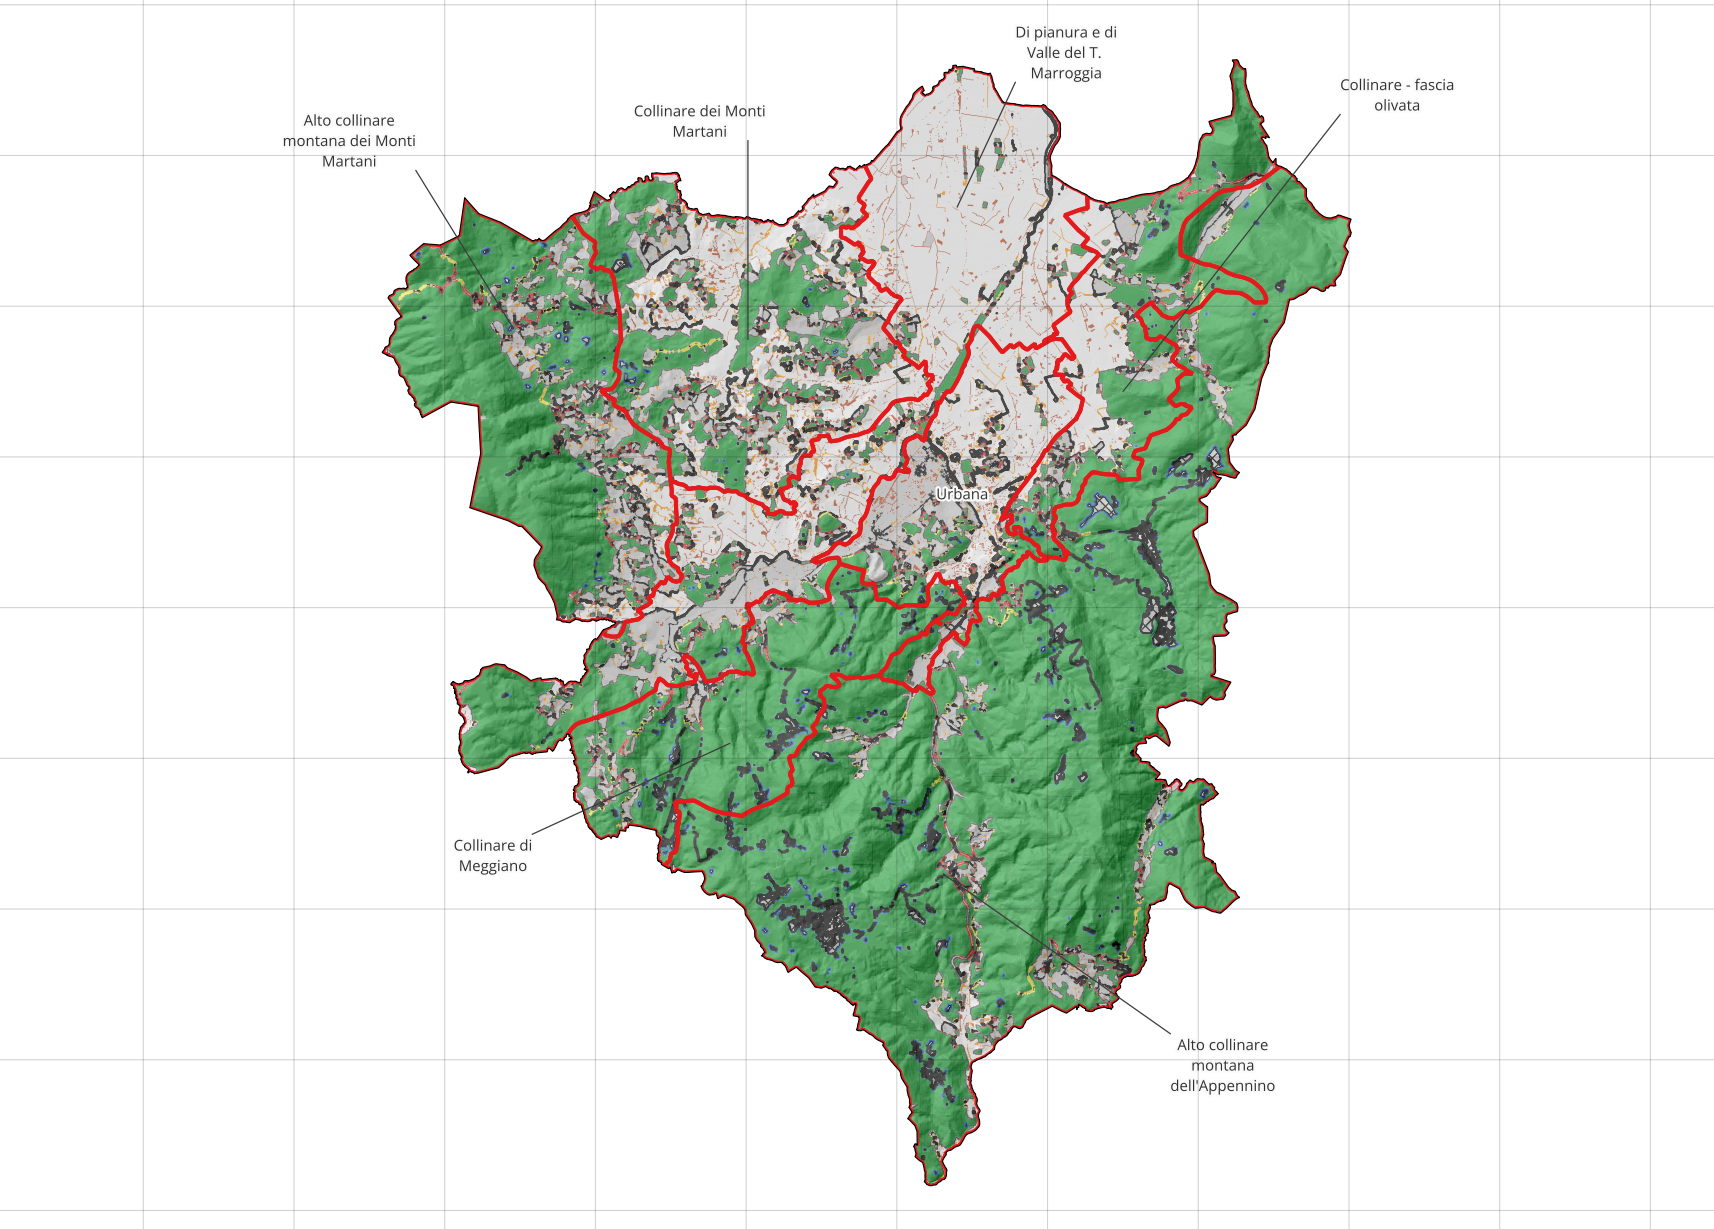
\includegraphics[width=\linewidth]{./figs/mspa_unitaFunzionali} 

}

\caption{Riclassificazione del territorio comunale secondo il metodo MSPA e ripartizione in unità funzionali.}\label{fig:mspaUnitaFunzionali}
\end{figure}

\subsubsection{Aree Montane e Dorsali Appenniniche (UF Alto collinare montana dell'Appennino e Alto collinare montana dei Monti Martani)}\label{aree-montane-e-dorsali-appenniniche-uf-alto-collinare-montana-dellappennino-e-alto-collinare-montana-dei-monti-martani}

In queste unità come era atteso sono presenti i valori di gran lunga più elevati di Area Totale e Effective Mesh Size per la classe \emph{Core} (Fig. \ref{fig:mspaUnitaFunzionaliMontana})(Tab x).
Questo evidenzia un paesaggio a matrice prevalentemente naturale, dove l'habitat è continuo e poco frammentato.
Queste unità presentano i valori di gran lunga più elevati di Area Totale e Effective Mesh Size per la classe \emph{Core}.
Questo evidenzia un paesaggio a matrice prevalentemente naturale, dove l'habitat è continuo e poco frammentato.
Inoltre, l'elevato valore di \(S_{eff}\) corrispondente a XX nei \emph{Core} conferma che le aree core non sono solo estese, ma strutturate in macro-blocchi compatti, ideali per la conservazione della biodiversità ad ampio raggio.

Riguardo le Componenti di Margine e i Corridoi, i valori di \emph{Bridge} ed \emph{Edge} mostrano un'estensione significativa ma un \(S_{eff}\) contenuto rispetto ai \emph{Core}, indicando che la matrice boschiva è continua e presenta margini esterni ben definiti senza eccessiva perforazione interna.

\begin{figure}

{\centering 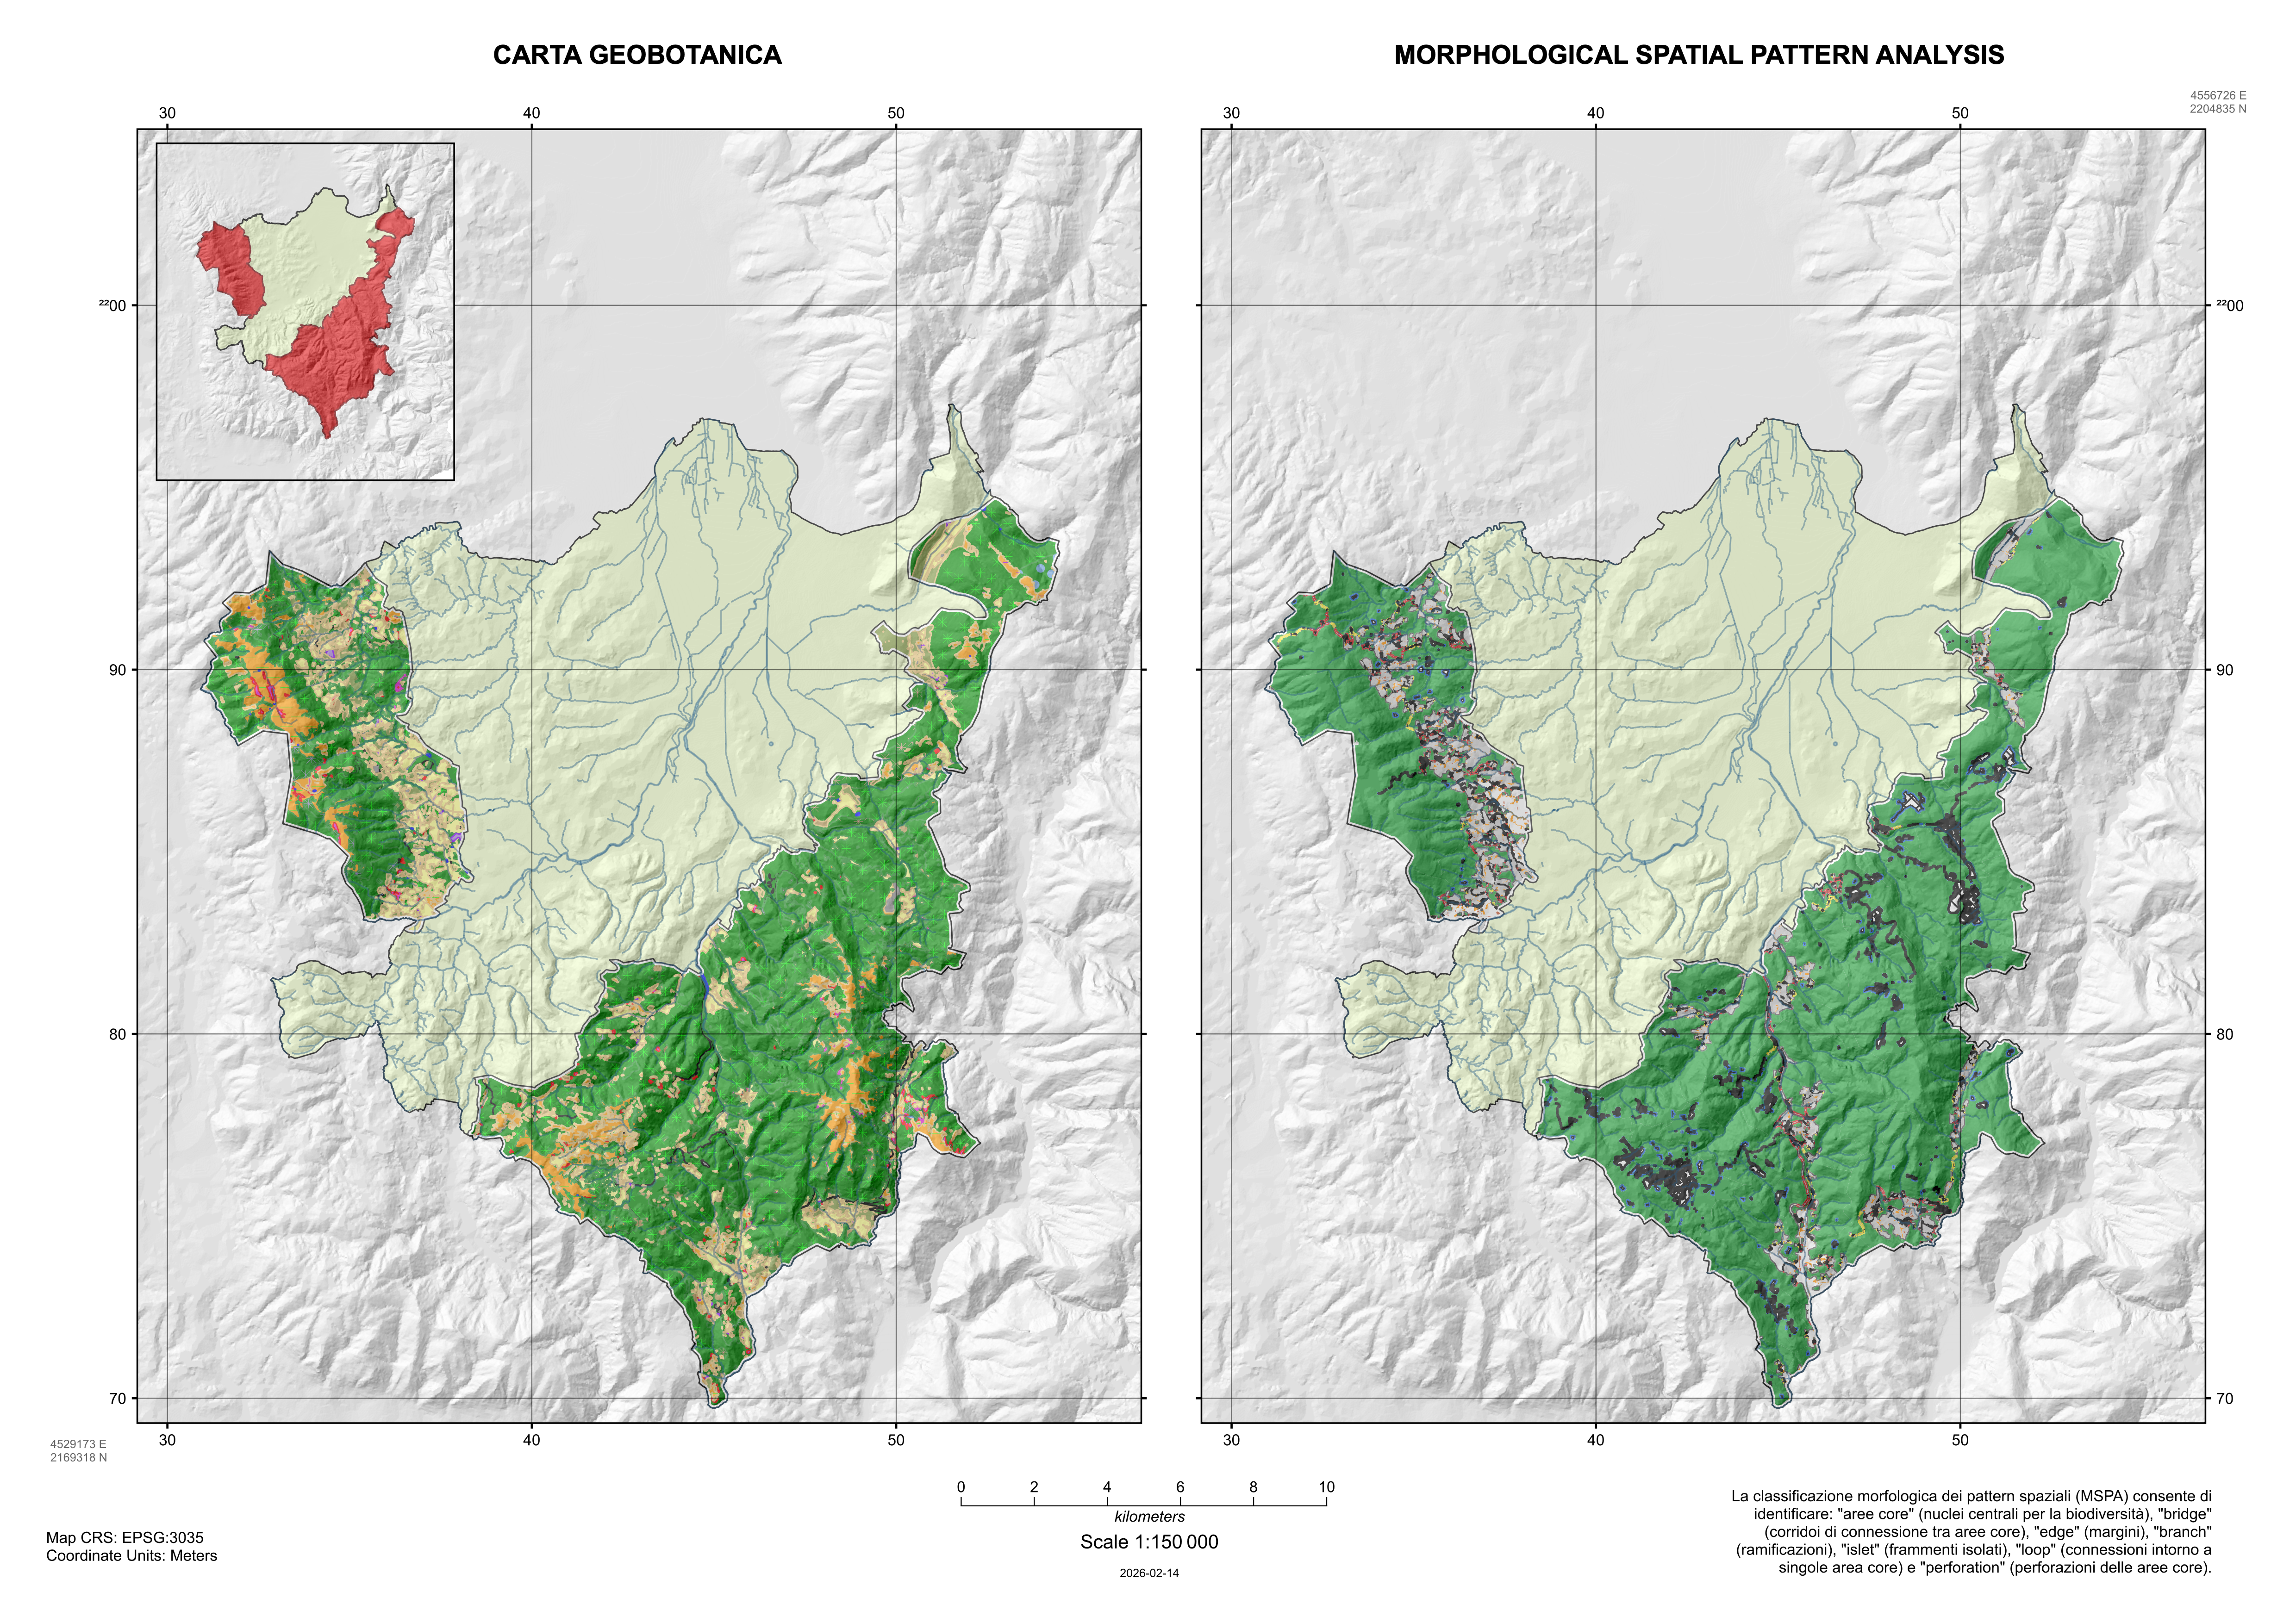
\includegraphics[width=\linewidth]{./figs/mspa_unitaFunzionali_montana} 

}

\caption{Carta geobotanica e analisi MSPA delle unità funzionali Alto collinare montana dell'Appennino e Alto collinare montana dei Monti Martani}\label{fig:mspaUnitaFunzionaliMontana}
\end{figure}

\subsubsection{Fasce di Transizione Pedemontane e Collinari (UF Collinare fascia olivata, Collinare dei Monti Martani, Collinare di Meggiano)}\label{fasce-di-transizione-pedemontane-e-collinari-uf-collinare-fascia-olivata-collinare-dei-monti-martani-collinare-di-meggiano}

In queste aree l'area \emph{Core} si riduce notevolmente a favore di una maggiore presenza proporzionale di \emph{Edge}, \emph{Branch}, \emph{Loop} e \emph{Bridge} (Figg. \ref{fig:mspaUnitaFunzionaliOlivata}; \ref{fig:mspaUnitaFunzionaliCollinare}; Tab x).
Infatti, la presenza diffusa di \emph{Bridge} e \emph{Branch} testimonia una rete di siepi, formazioni ripariali e lembi boschivi interconnessi con la matrice agricola/olivicola.
Tuttavia, il basso valore di \(S_{eff}\) segnala che tali elementi sono frequentemente suddivisi in brevi tratti, vulnerabili all'effetto margine e all'interruzione di continuità.
Inoltre, la presenza di \emph{Perforation} evidenzia l'effetto dell'attività antropica o dell'uso agricolo che penetra all'interno dei margini boschivi residui.

\begin{figure}

{\centering 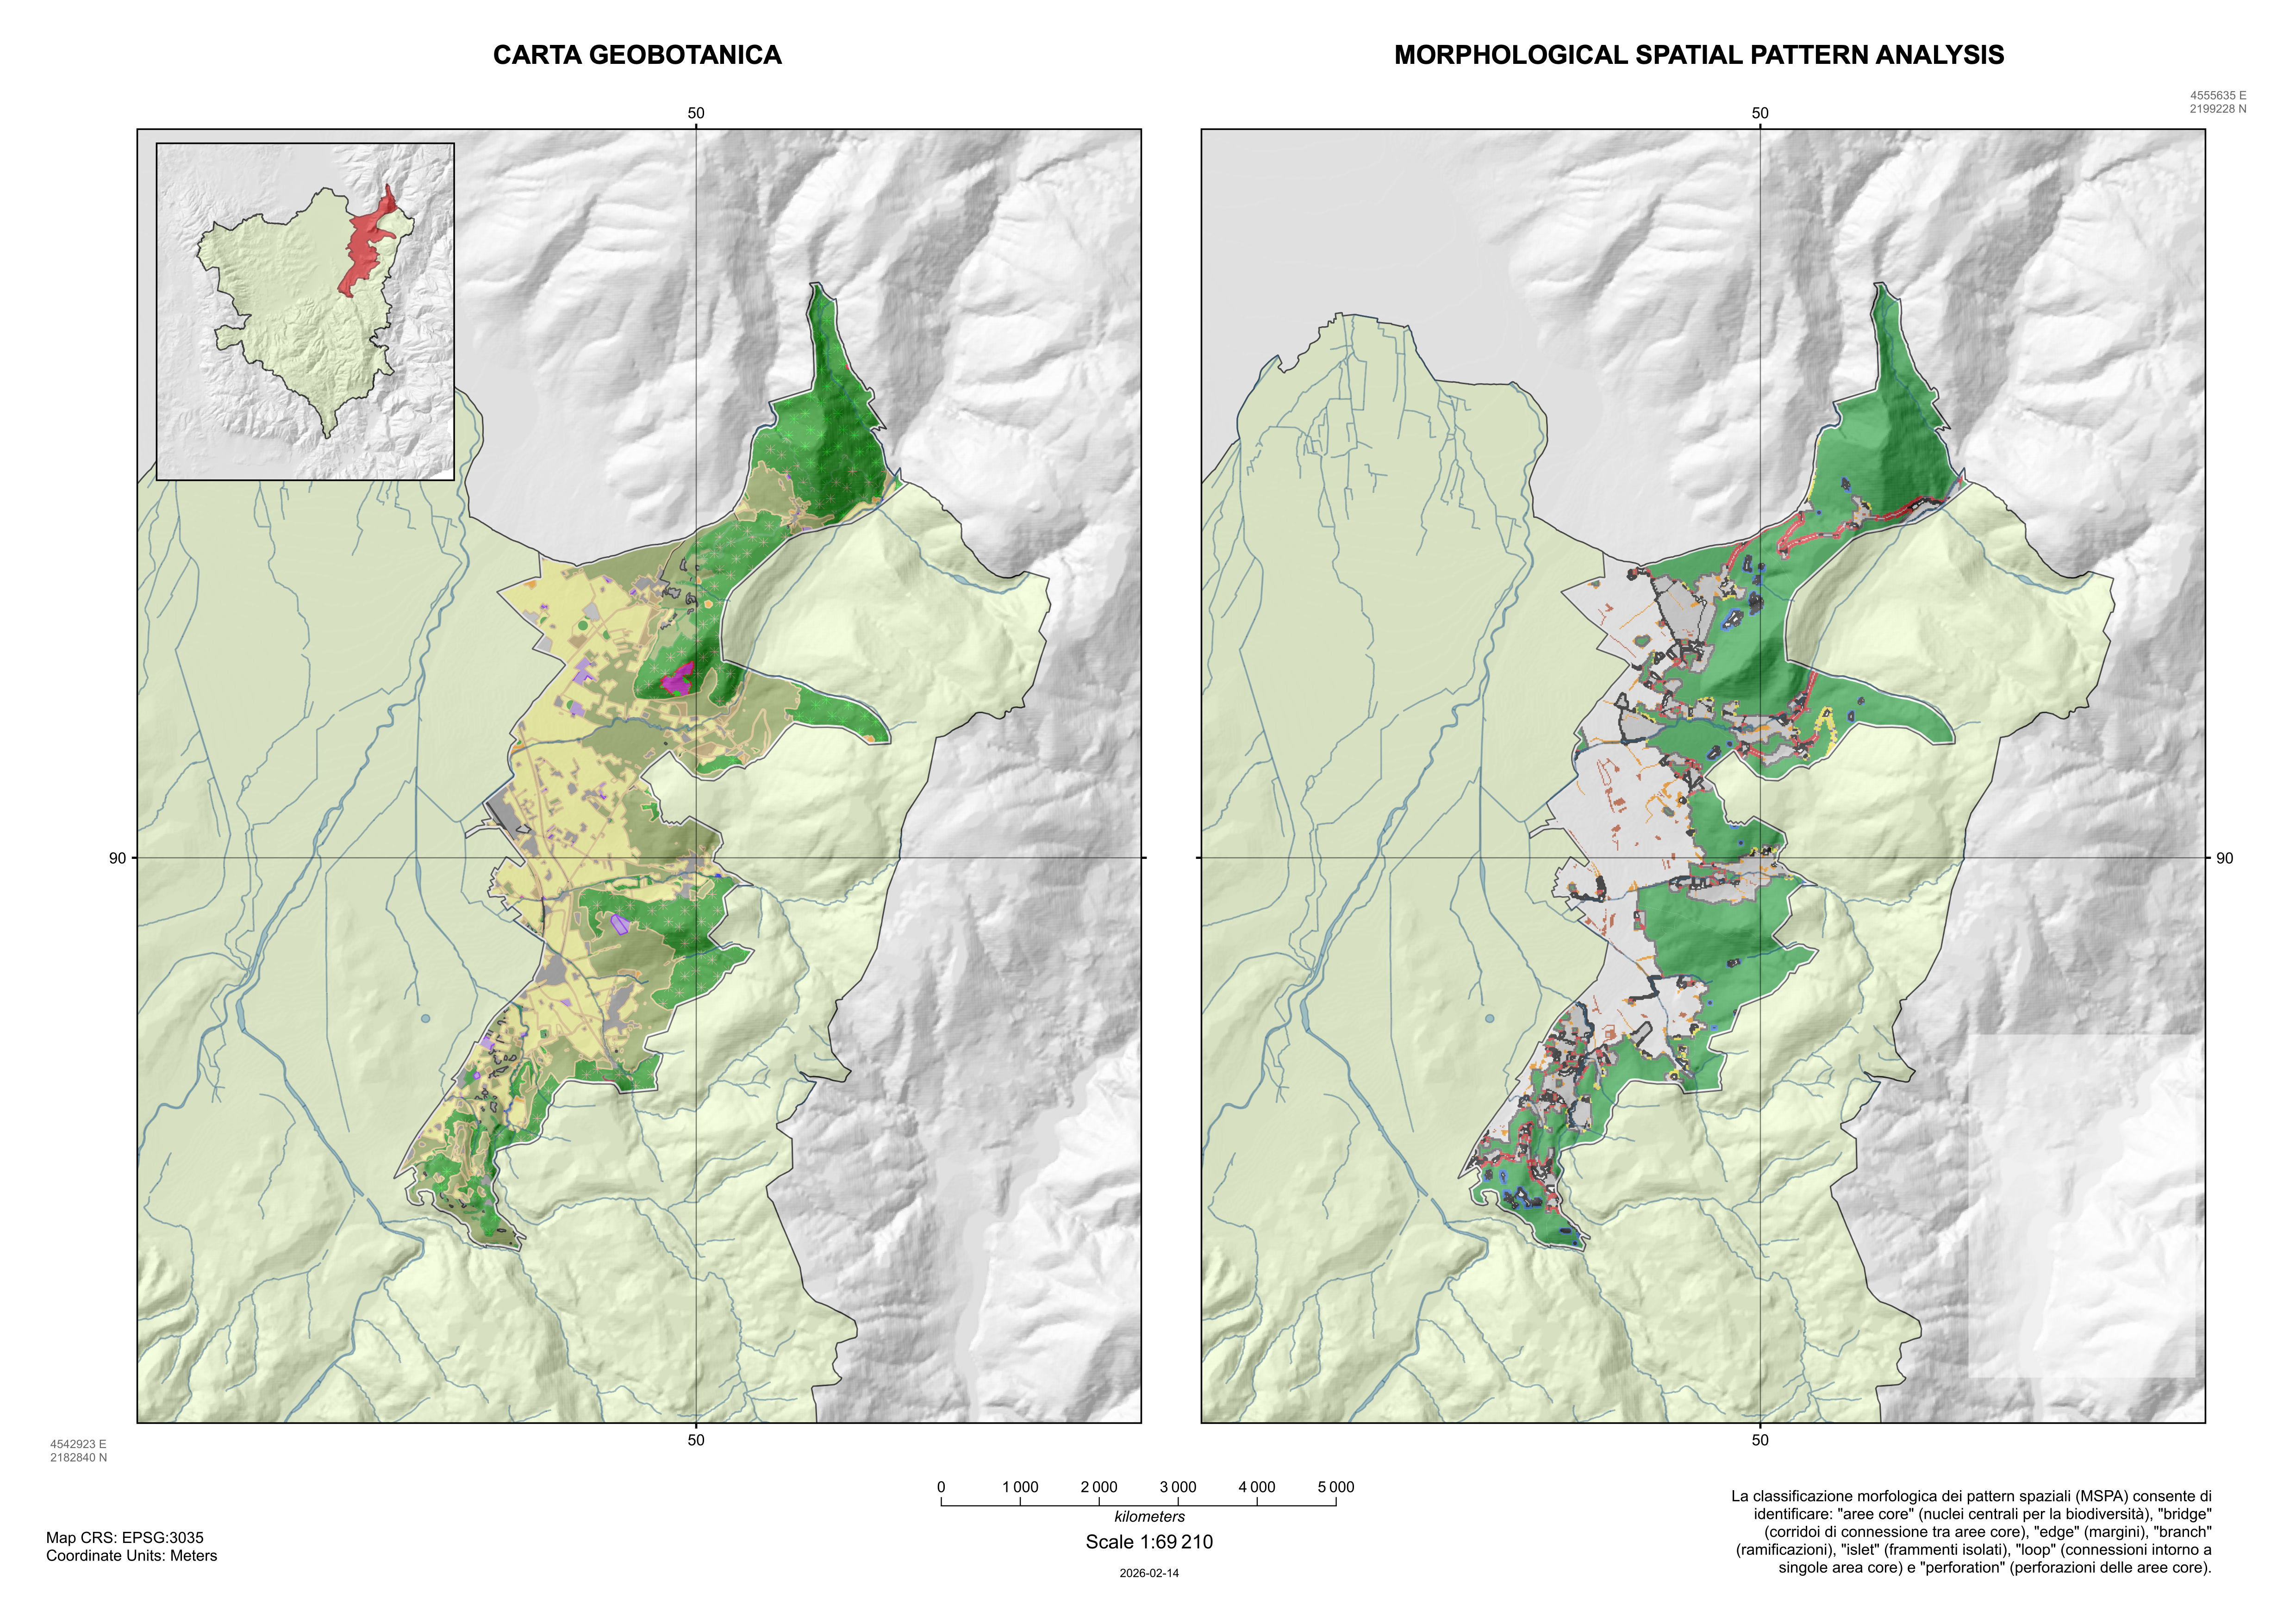
\includegraphics[width=\linewidth]{./figs/mspa_unitaFunzionali_olivata} 

}

\caption{Carta geobotanica e analisi MSPA dell'unità funzionale Collinare fascia olivata}\label{fig:mspaUnitaFunzionaliOlivata}
\end{figure}

\begin{figure}

{\centering 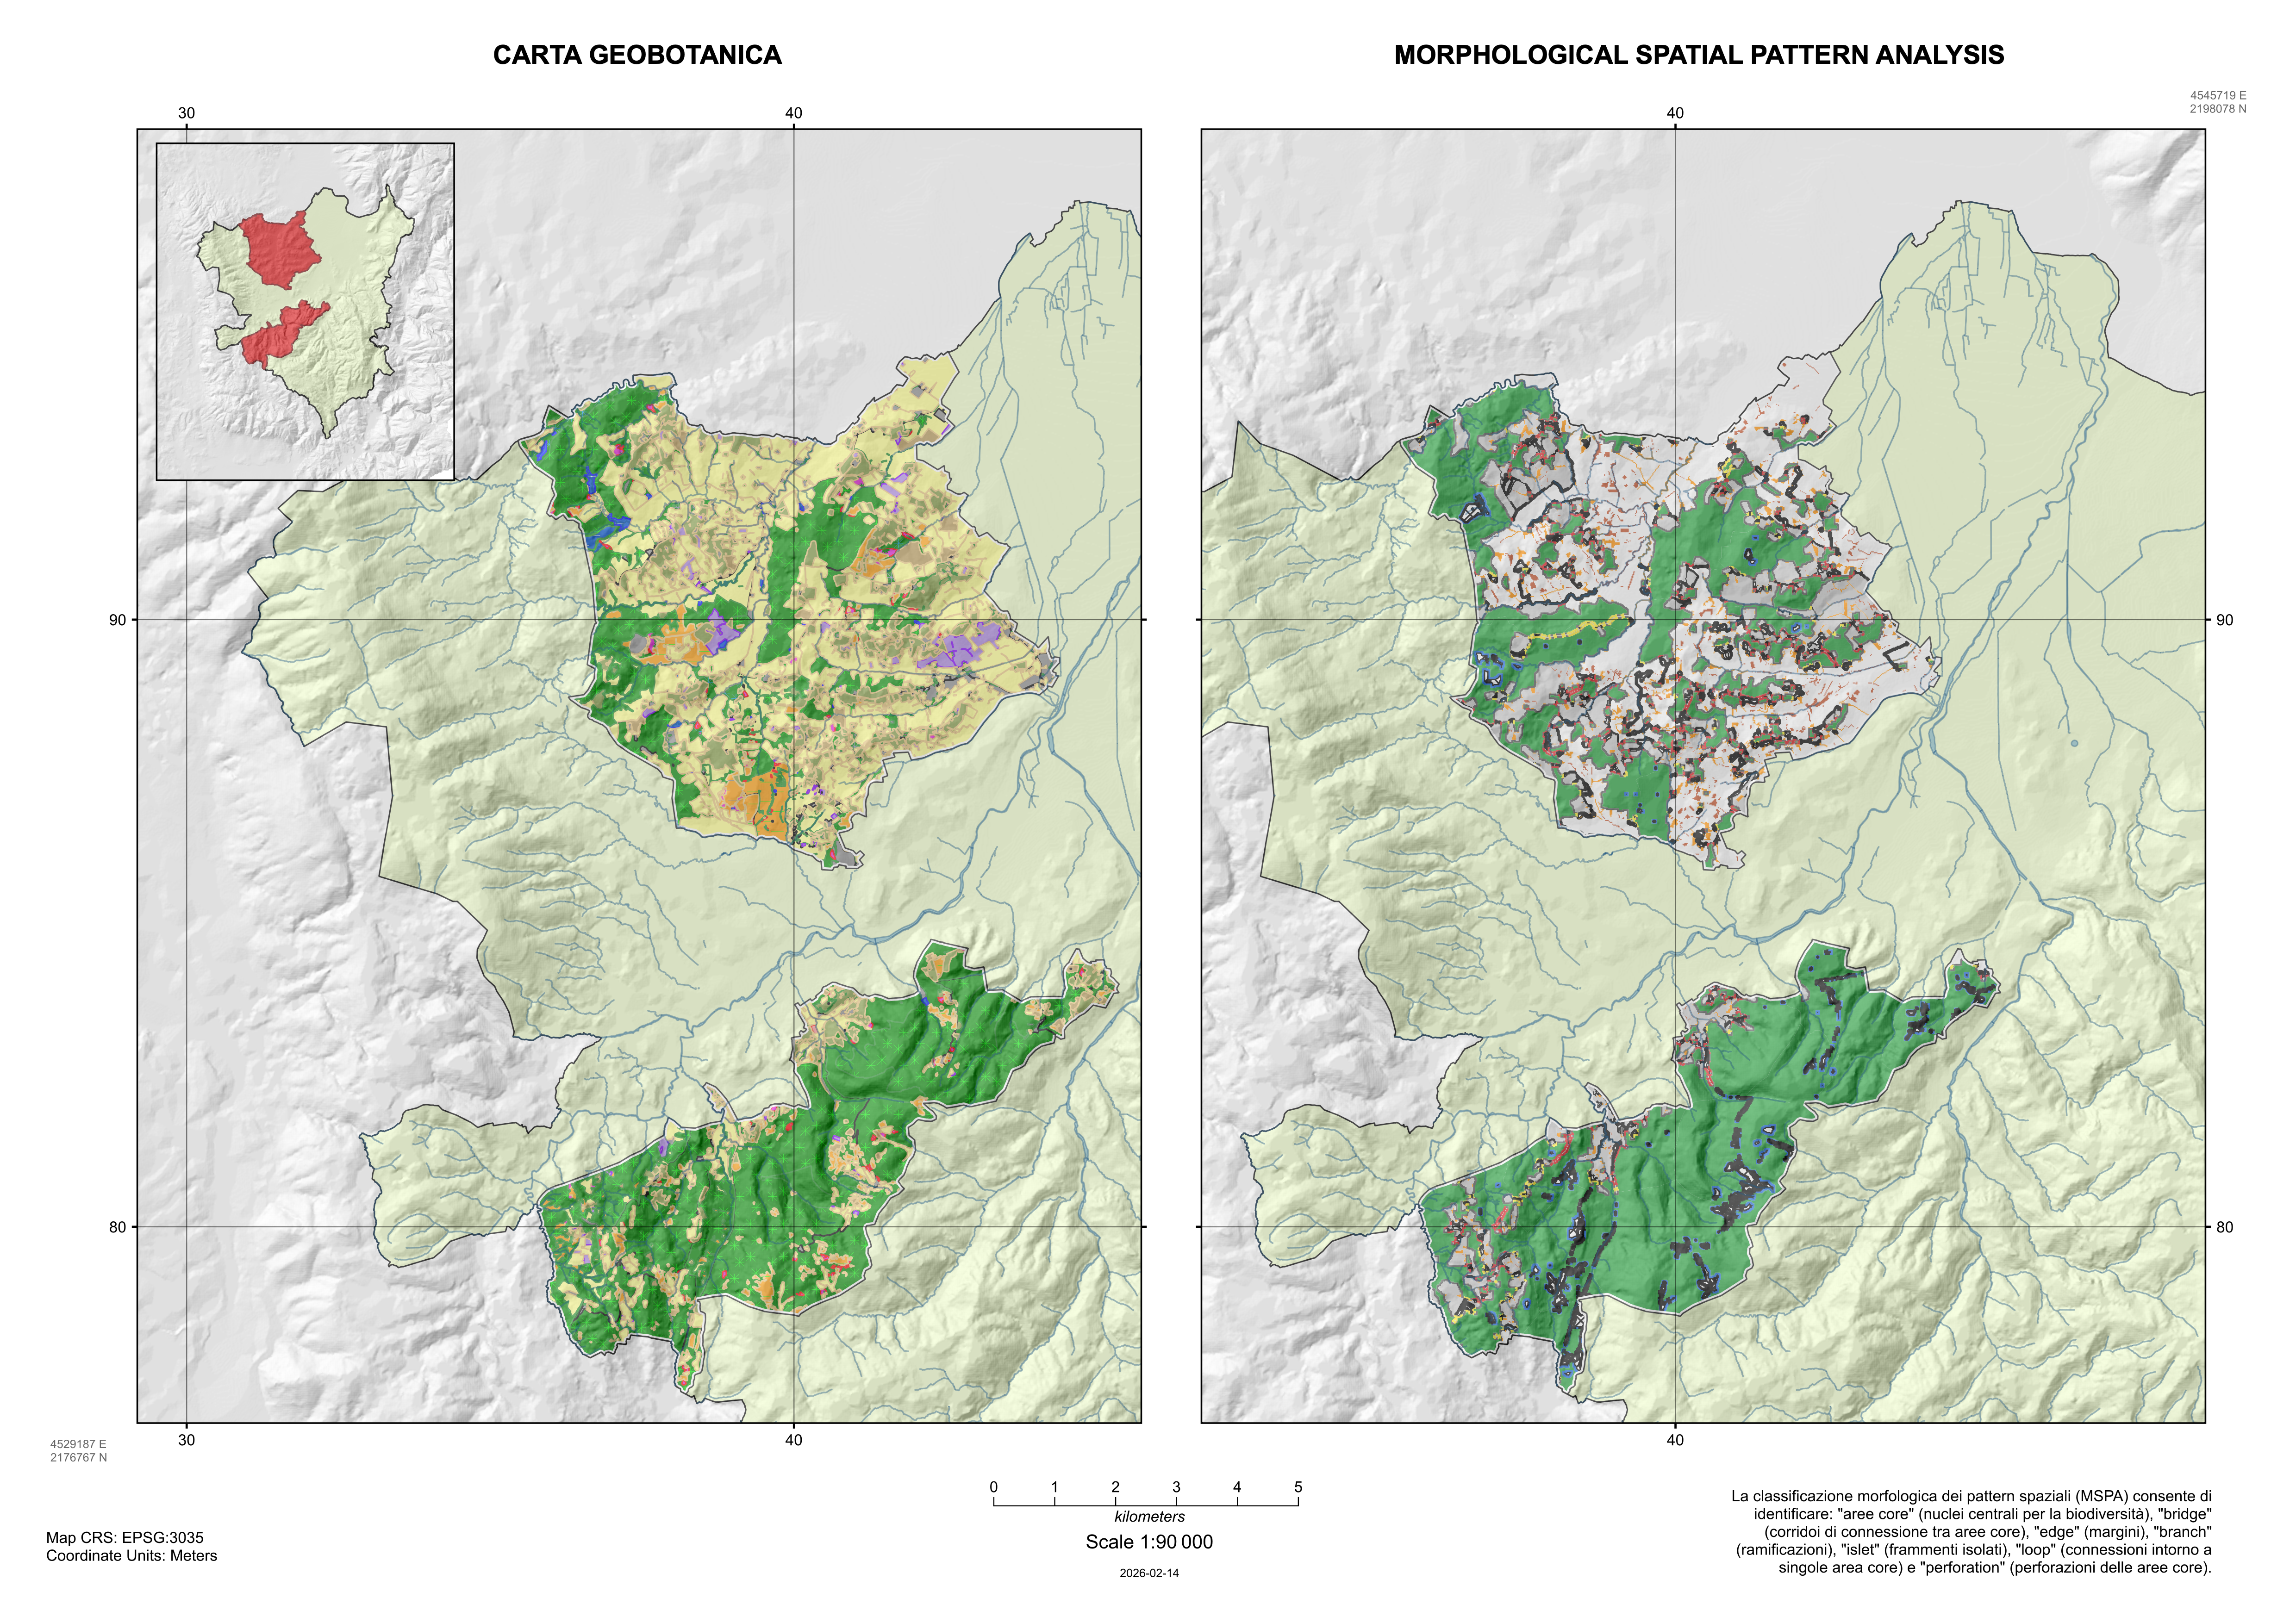
\includegraphics[width=\linewidth]{./figs/mspa_unitaFunzionali_collinare} 

}

\caption{Carta geobotanica e analisi MSPA delle unità funzionali Collinare dei Monti Martani, Collinare di Meggiano}\label{fig:mspaUnitaFunzionaliCollinare}
\end{figure}

\subsubsection{Area di pianura e di valle (UF di pianura e di Valle del T. Marroggia)}\label{area-di-pianura-e-di-valle-uf-di-pianura-e-di-valle-del-t.-marroggia}

In quest'area si osserva una presenza marcata della classe \emph{Islet} (piccole patches isolate) unitamente a significativi valori di \emph{Bridge} rappresentati dai corridoi fluviali e dal reticolo idrografico minore (Fig. \ref{fig:mspaUnitaFunzionaliValle}; Tab.
x).
Nonostante l'Area Totale per \emph{Bridge} o \emph{Islet} sia rilevante, il relativo \(S_{eff}\) è decisamente basso.
Ciò dimostra che la connettività ecologica in fondo valle è affidata a corridoi stretti e frammentati, fortemente condizionati dalla pressione delle infrastrutture e dell'urbanizzazione.

\begin{figure}

{\centering 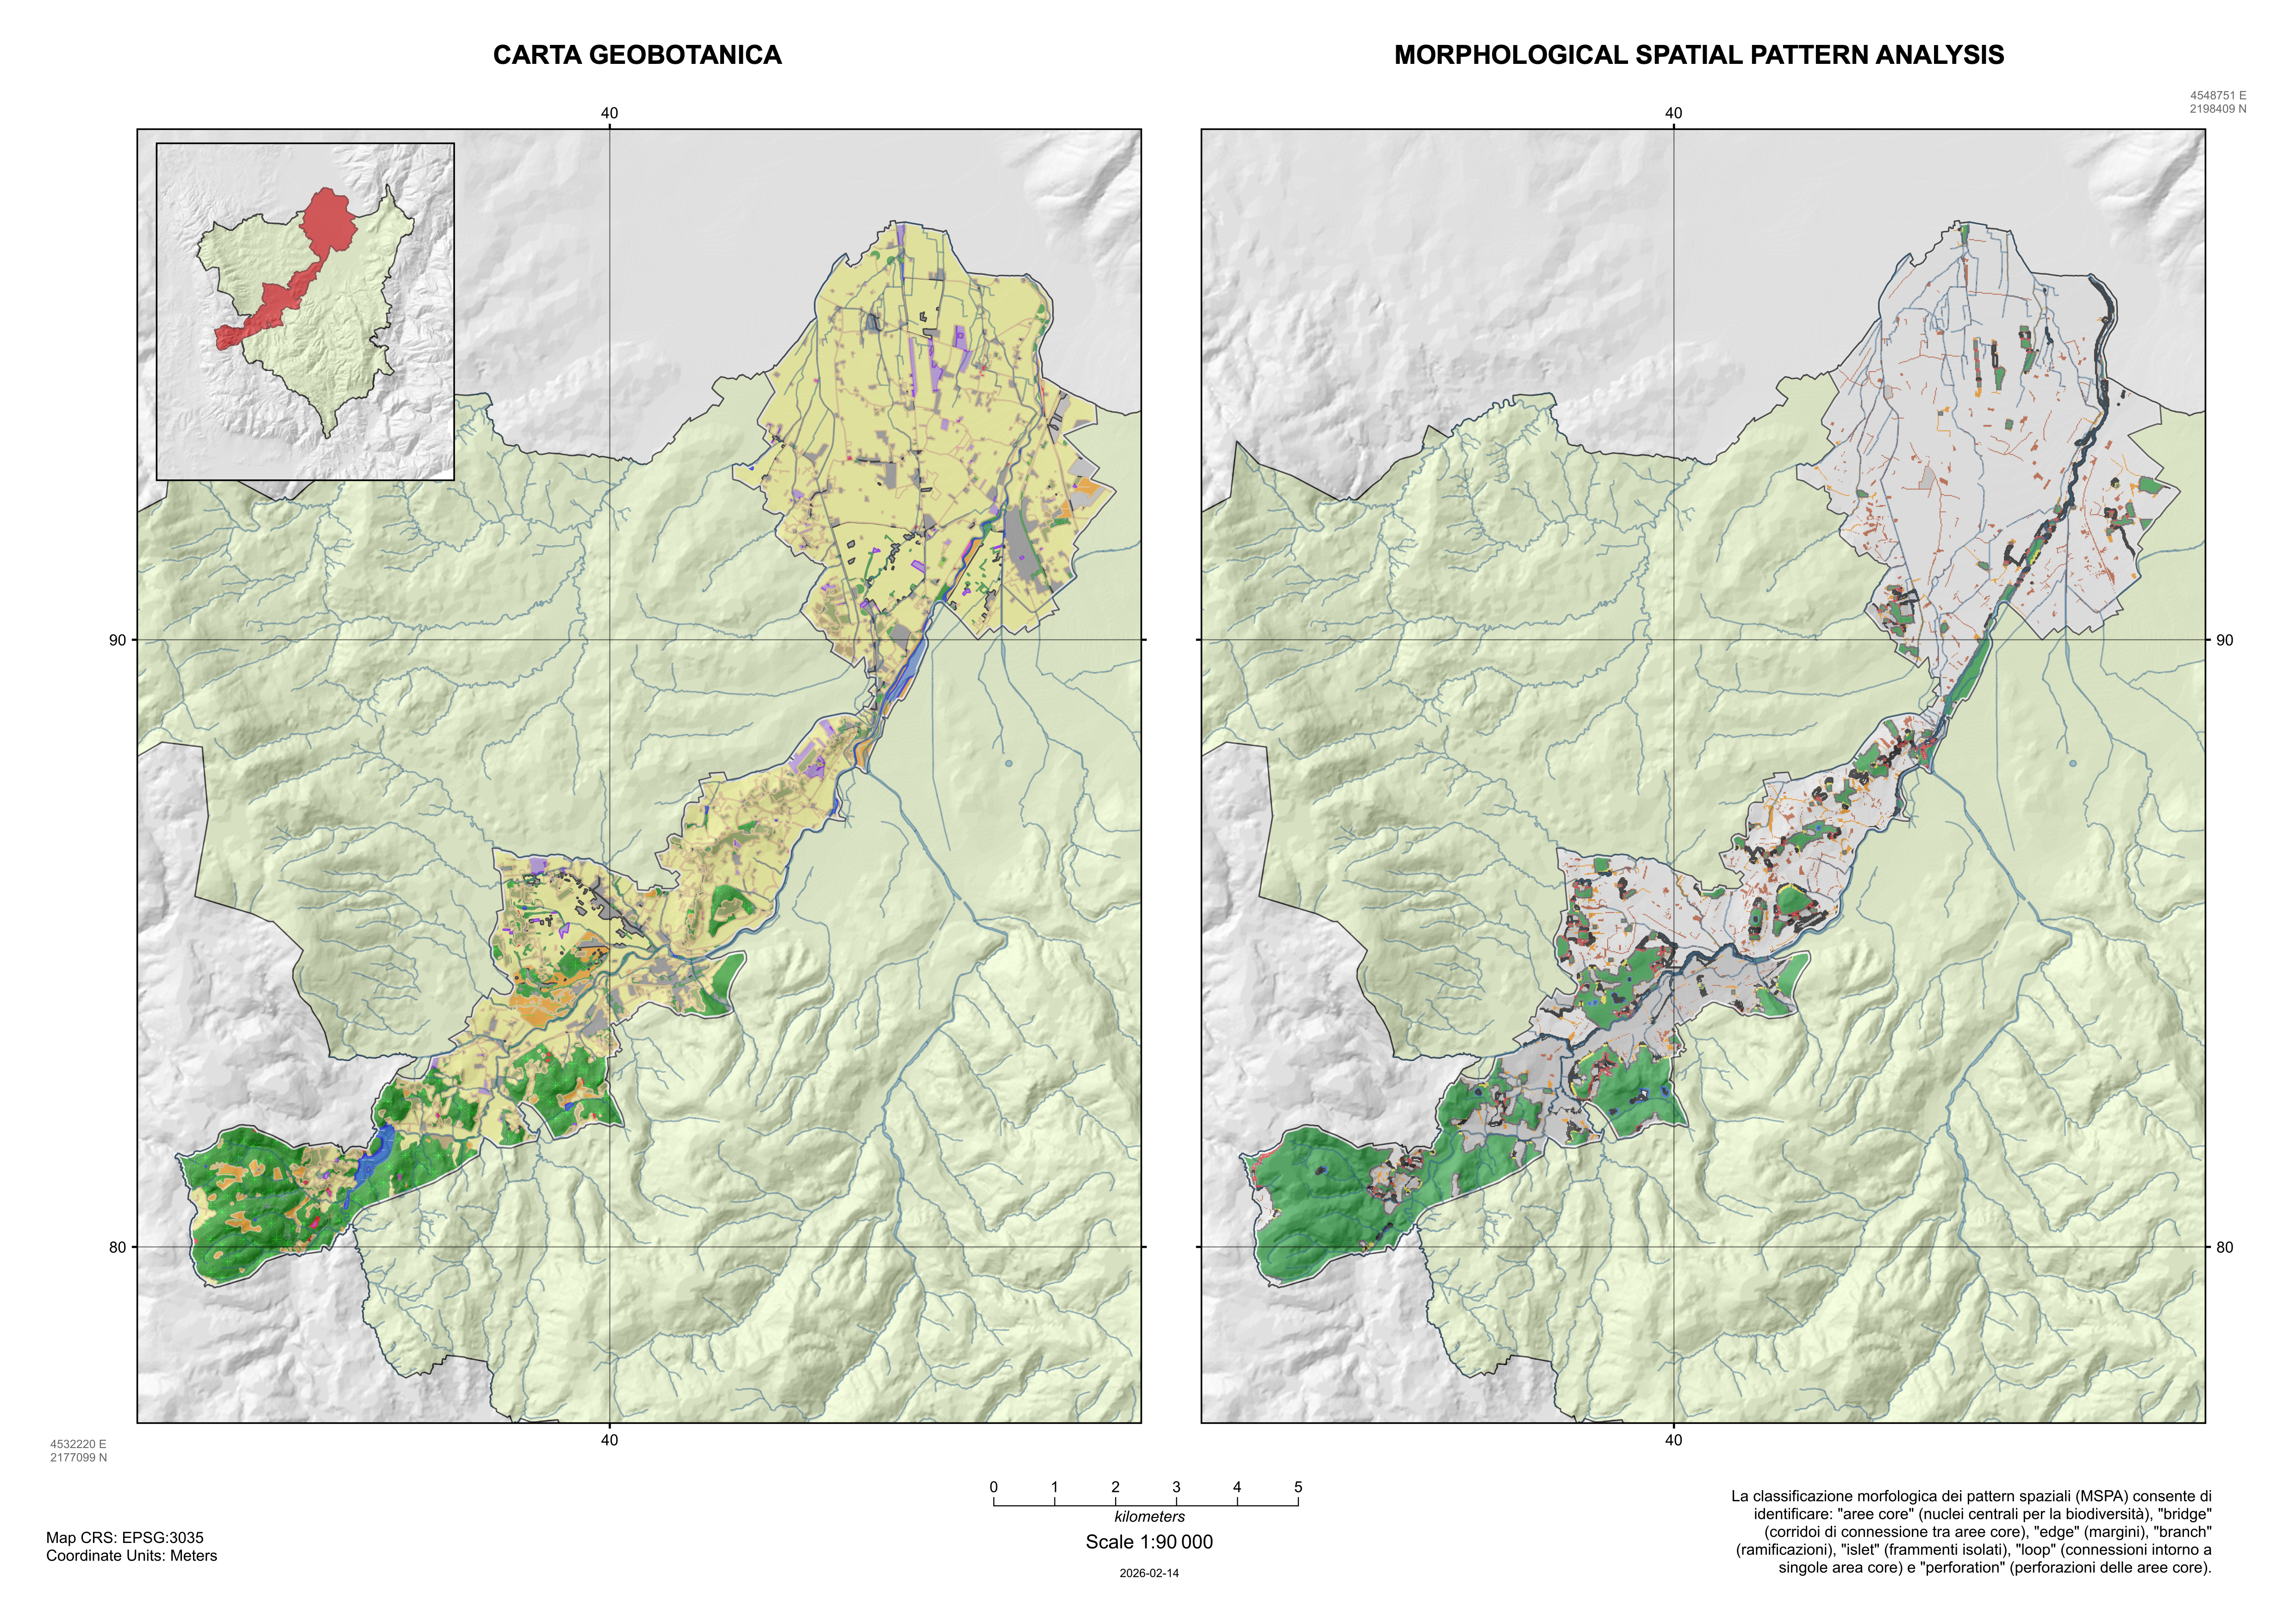
\includegraphics[width=\linewidth]{./figs/mspa_unitaFunzionali_valle} 

}

\caption{Carta geobotanica e analisi MSPA dell'unità funzionale di pianura e di Valle del T. Marroggia}\label{fig:mspaUnitaFunzionaliValle}
\end{figure}

\subsubsection{Ambito Urbano / Antropizzato (UF Urbana)}\label{ambito-urbano-antropizzato-uf-urbana}

Come atteso, l'area \emph{Core} in questa UF è poco rappresentata.
Prevalgono elementi isolati (\emph{Islet}) e i corridoi a fondo cieco (\emph{Branch}) (Fig. \ref{fig:mspaUnitaFunzionaliUrbana}; Tab x).
L'Effective Mesh Size assume i valori più bassi dell'intero territorio comunale per quasi tutte le categorie ecologiche funzionali, confermando una matrice urbana poco permeabile al movimento della fauna con un basso livello di continuità degli habitat naturali.

\begin{figure}

{\centering 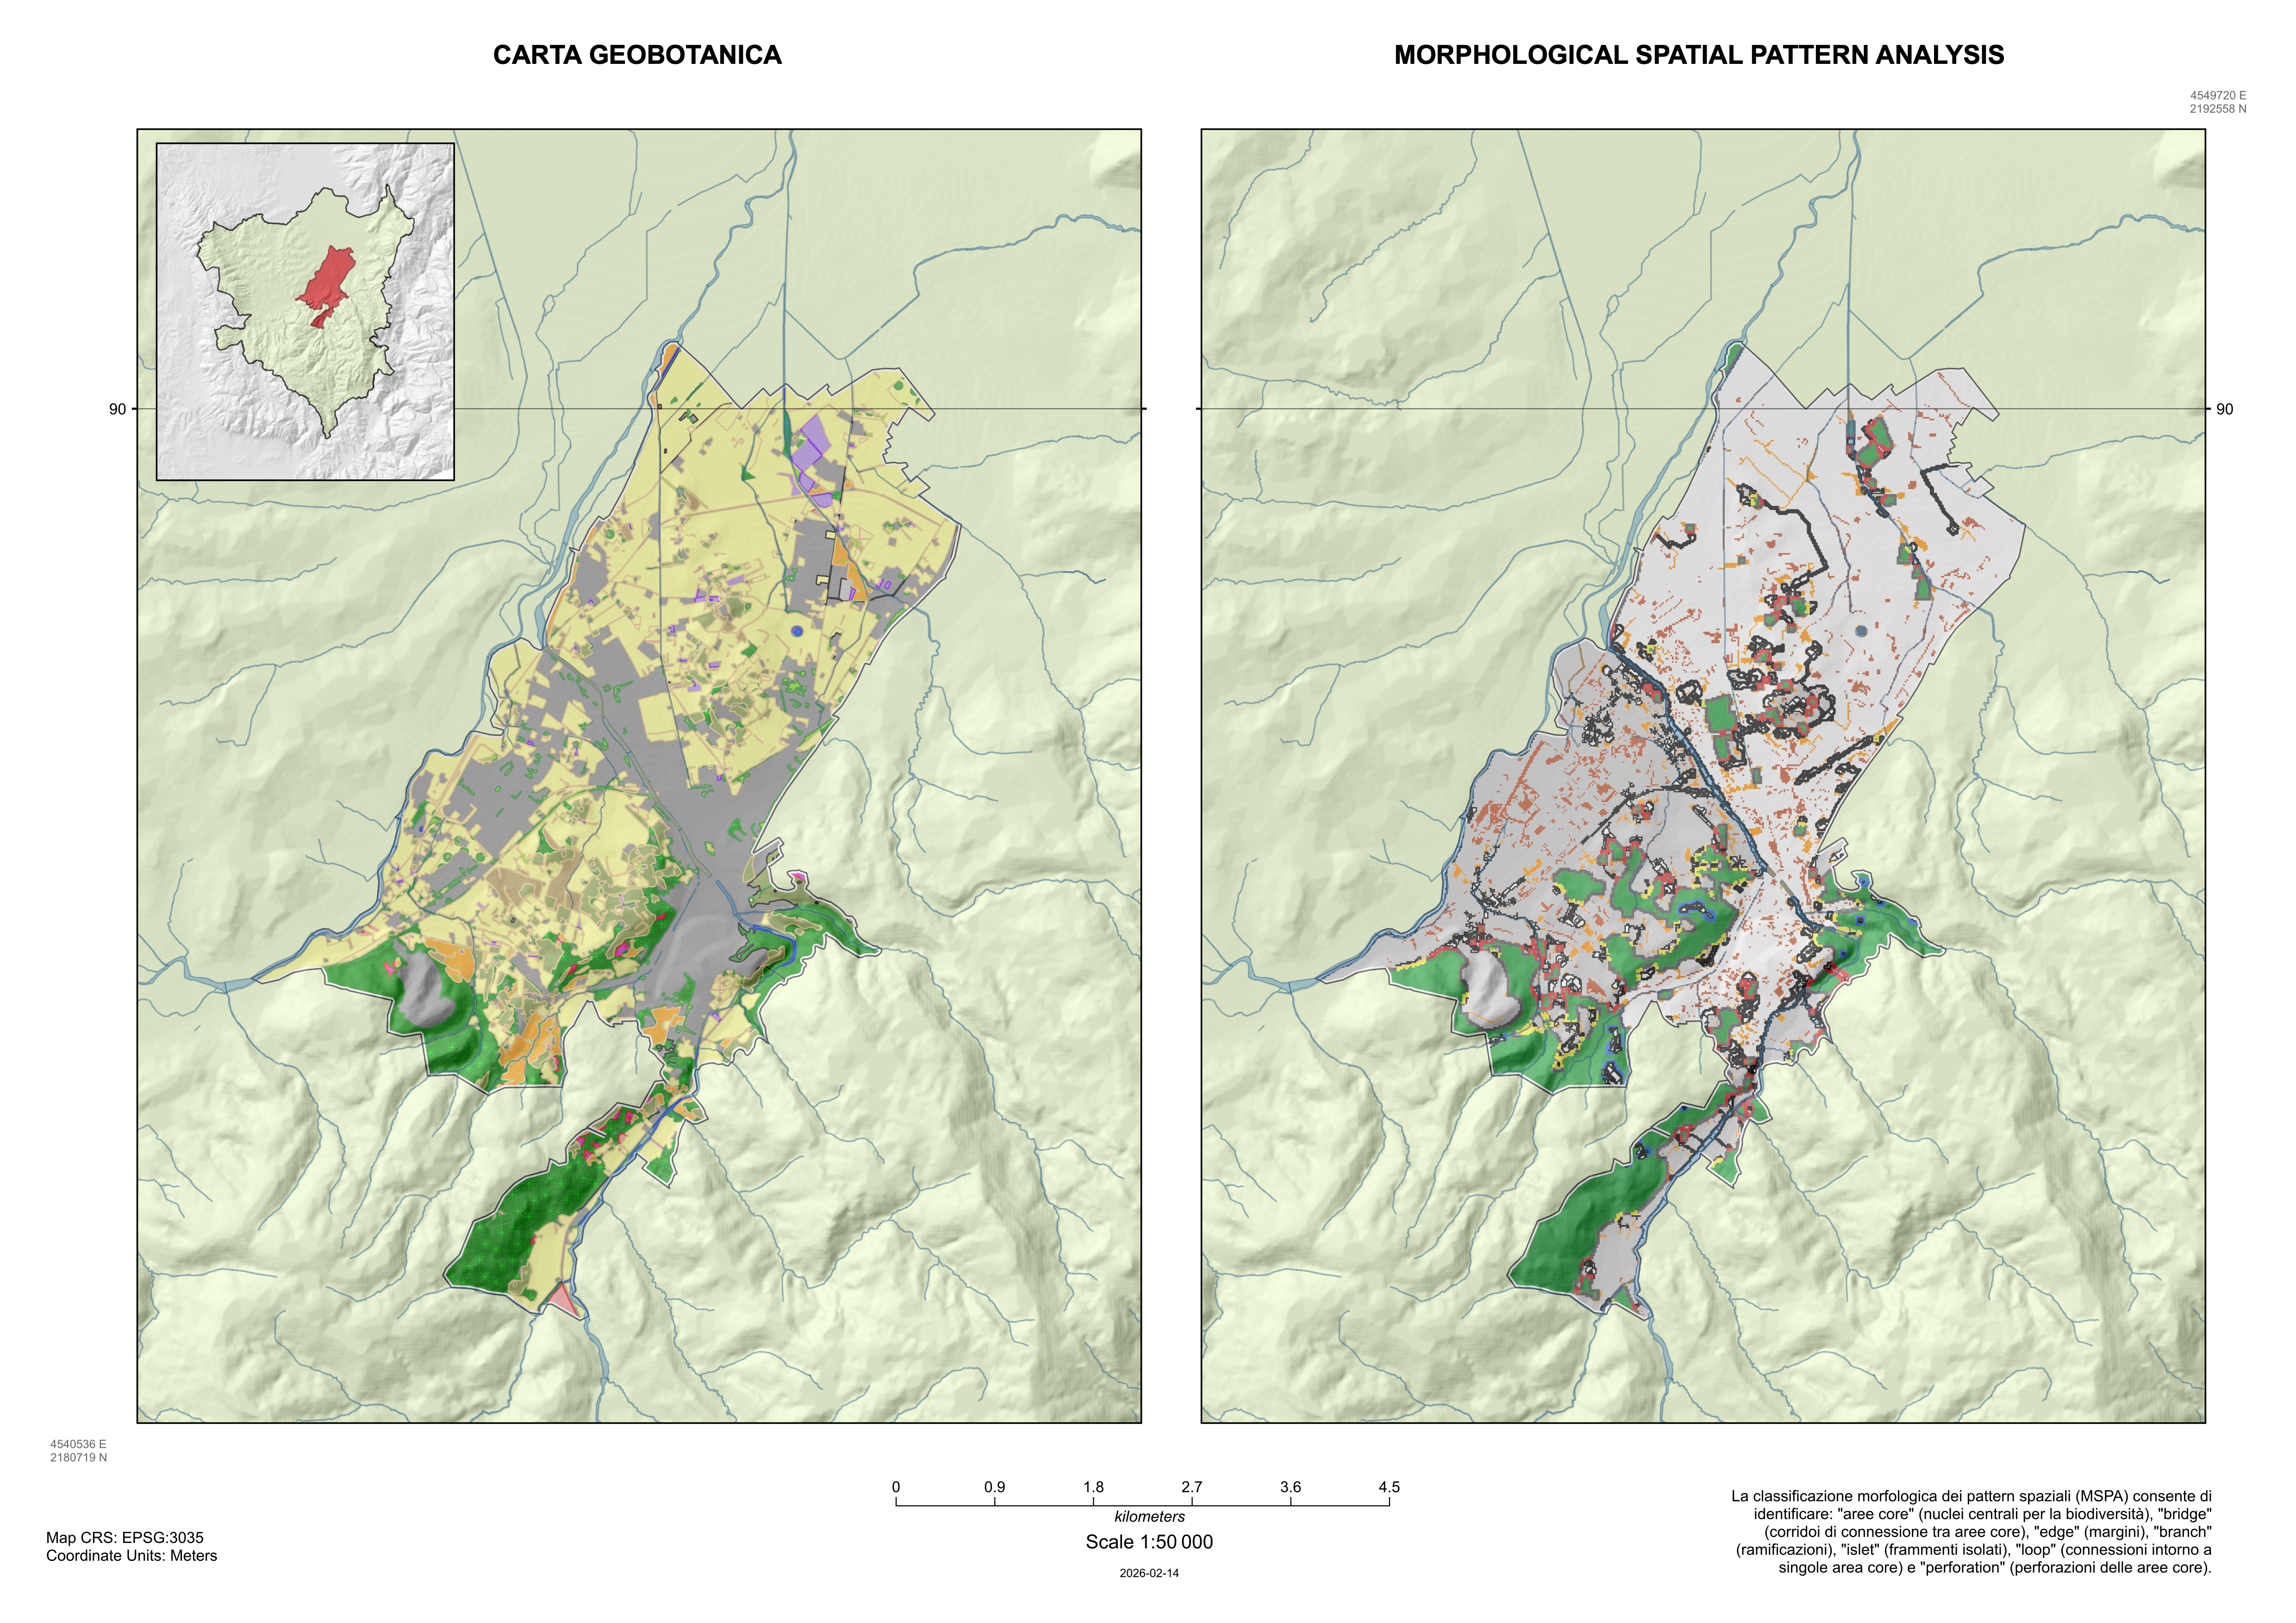
\includegraphics[width=\linewidth]{./figs/mspa_unitaFunzionali_urbana} 

}

\caption{Carta geobotanica e analisi MSPA dell'unità funzionale urbana.}\label{fig:mspaUnitaFunzionaliUrbana}
\end{figure}

\subsubsection{Sintesi del confronto tra le Unità Funzionali}\label{sintesi-del-confronto-tra-le-unituxe0-funzionali}

In sostanza, il confronto tra le Unità Funzionali evidenzia una qualche forma di polarizzazione del territorio:

\begin{enumerate}
\def\labelenumi{\arabic{enumi}.}
\tightlist
\item
  Unità Montane: Funzionano da serbatoi di connettività (\emph{Source}) caratterizzati da elevate dimensioni della maglia utile (\(S_{eff}\)) e grandi blocchi \emph{Core}.
\item
  Unità Collinari e di fondo valle: Funzionano da vettori di transizione e corridoi ecologici (\emph{Stepping stones} e \emph{Bridges}), essenziali per il collegamento comunale e anche di scala regionale, ma soggetti a elevato rischio di frammentazione strutturale e funzionale.
\item
  Ambito Urbano: Rappresenta il contesto a maggior grado di criticità ecologica e isolamento. La rete ecologica residua in ambito urbano si fonda quasi esclusivamente su piccole chiazze isolate (Islet) e bracci ciechi (Branch), evidenziando la necessità prioritario-gestionale di interventi di deframmentazione e re-infrastrutturazione verde (es. corridoi urbani, stepped stepping stones e forestazione urbana) per mantenere un minimo livello di permeabilità ecologica.
\end{enumerate}

\section{Composizione e struttura del sistema verde e blu}\label{composizione-e-struttura-del-sistema-verde-e-blu}

\subsection{Estensione e composizione}\label{estensione-e-composizione}

Come anticipato nelle premesse metodologiche, lo studio ha previsto una valutazione puntuale delle infrastrutture verdi e blu, tenendo conto sia della componente privata che pubblica. La mappa della loro distribuzione spaziale complessiva è riportata in figura \ref{fig:verdeSpoleto}.

\begin{figure}

{\centering 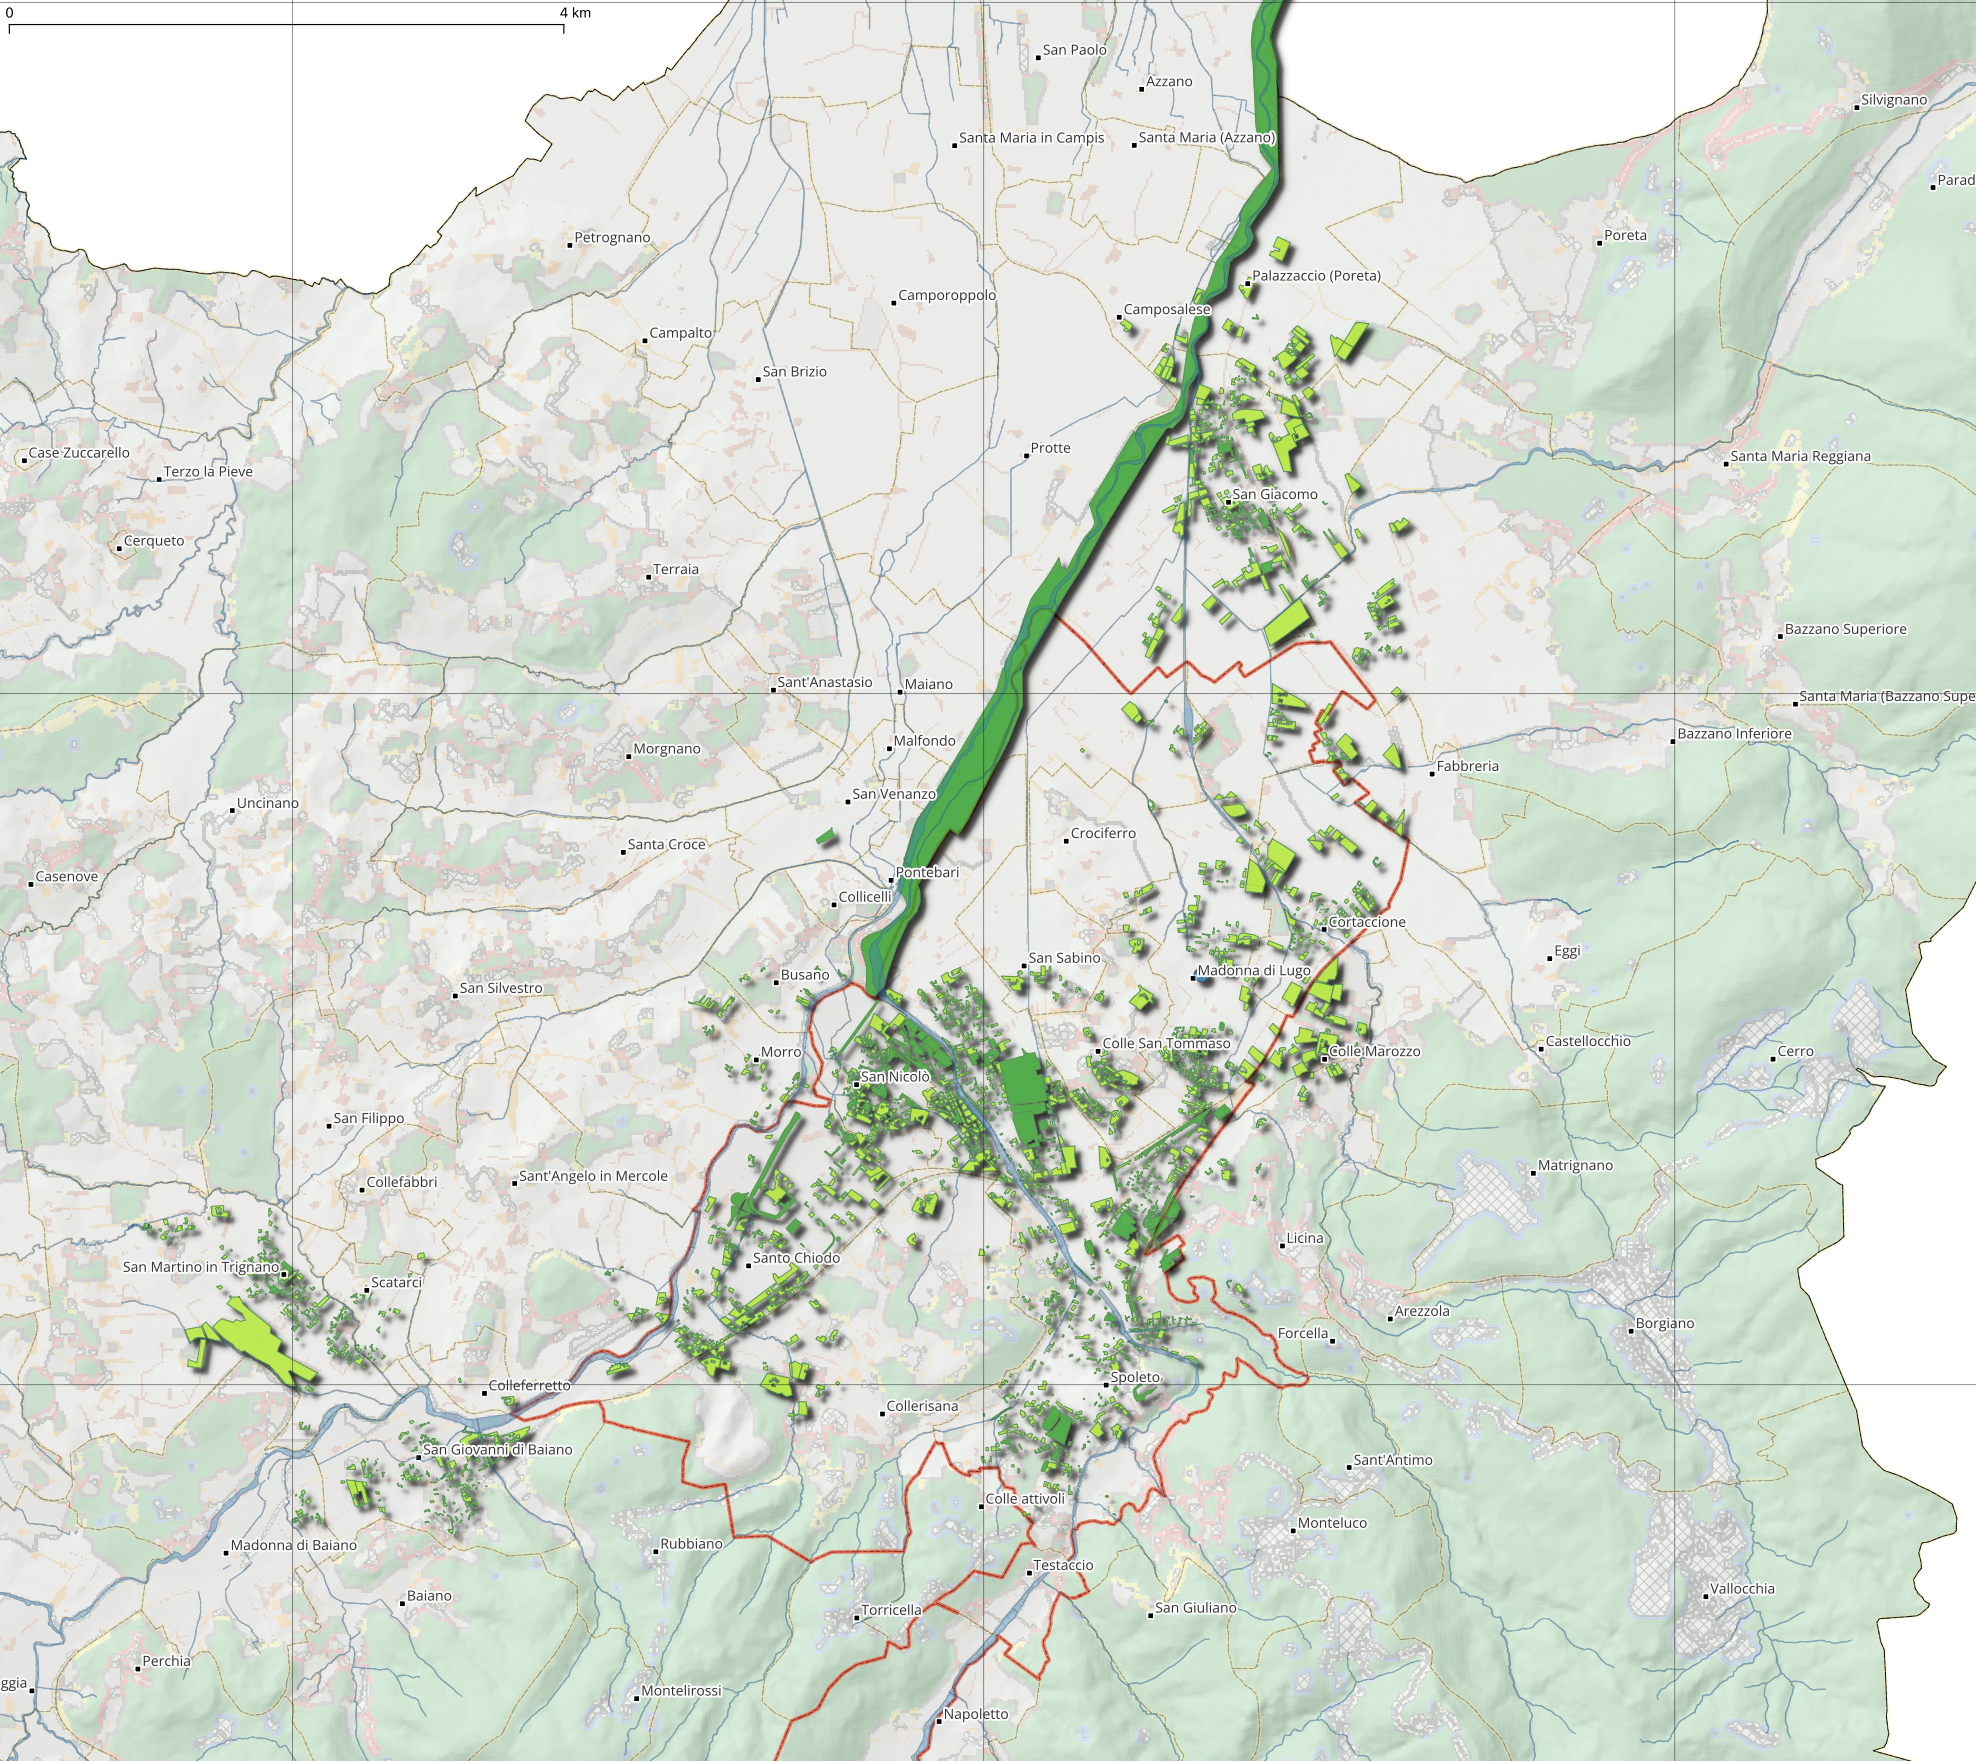
\includegraphics[width=\linewidth]{./figs/verdeSpoleto} 

}

\caption{Carta del verde (pubblico in tonalità scura e privato in tonalità più chiara) e del reticolo fluviale. Sullo sfondo in sovrapposizione la mappa MSPA sfumata. Il confine dell'unità funzionale urbana è evidenziato in rosso.}\label{fig:verdeSpoleto}
\end{figure}

Focalizzando l'attenzione alla sola area urbana, definita secondo il modello delle unità funzionali (cfr. capitolo unità funzionali) e per la quale si dispone di una cartografia sufficientemente dettagliata e accurata nella rappresentazione degli elementi del verde, si nota che la composizione degli elementi delle infrastrutture verdi e blu occupano una superficie totale di quasi 200 ha.
Tale valore corrisponde a circa il 12.5\% del territorio in esame.
Nella ripartizione tra verde pubblico/privato e aree blu la componente privata rappresenta il 61\% del totale e il blu solamente il 7\% (\ref{tab:verdeBase}).\footnote{L'analisi condotta mediante rasterizzazione della cartografia vettoriale mette in evidenza una lieve riduzione delle superfici rispetto ai valori originari. Tale differenza è piuttosto contenuta e imputabile alla trasformazione su maglia 5x5 m e alla successiva applicazione del limite dell'area di studio corrispondente all'unità funzionale urbana. Le differenze risultano contenute per il verde privato e per le componenti blu, mentre sono più evidenti per il verde pubblico, caratterizzato da numerosi elementi di piccola dimensione e geometrie articolate.}

\begin{longtable}[]{@{}llrrr@{}}
\caption{\label{tab:verdeBase} Metriche della composizione del verde urbano per tipologia.}\tabularnewline
\toprule\noalign{}
componente & proprieta & n\_poligoni & area\_ha & PLAND \\
\midrule\noalign{}
\endfirsthead
\toprule\noalign{}
componente & proprieta & n\_poligoni & area\_ha & PLAND \\
\midrule\noalign{}
\endhead
\bottomrule\noalign{}
\endlastfoot
blu & pubblico & 19 & 14.54 & 0.92 \% \\
verde & privato & 1171 & 117.83 & 7.67 \% \\
verde & pubblico & 255 & 60.41 & 3.94 \% \\
\textbf{Totale} & - & 1445 & 192.79 & 12.53 \% \\
\end{longtable}

Complessivamente la mosaicatura di queste infrastrutture si compone di 1445 poligoni, la maggior parte dei quali assimilabili al verde privato (79\%).

Dal punto di vista strutturale si osserva che le componenti verdi sono organizzate in un elevato numero di patch di piccole dimensioni, distribuite all'interno della matrice urbana, e caratterizzate da una superficie media di 0.84 ha.

\subsubsection{Configurazione spaziale e connettività}\label{configurazione-spaziale-e-connettivituxe0}

L'indice LPI corrispondente al Largest Patch Index raggiunge un valore pari a 87.3\%, indicando che la matrice territoriale dominante, costituita da infrastrutture grigie e da terreni agricoli, occupa gran parte della superficie totale.
In altre parole, come era atteso, il paesaggio risulta fortemente controllato dalla matrice urbana e dai seminativi che costituiscono lo sfondo all'interno del quale si distribuiscono gli elementi verdi e blu.

La superficie mediana delle patch di verde privato (3700 m\^{}2) è generalmente superiore a quella del verde pubblico (50 m\^{}2), suggerendo una maggiore presenza di nuclei vegetati continui all'interno delle proprietà private.
Nel verde pubblico e nei corsi d'acqua più della metà delle patch non supera due celle (circa 50 m\^{}2), e nel blu lo stesso vale per tre quarti delle patch.
Nel privato la mediana è 15 celle (circa 375 m\^{}2) e il terzo quartile 44 celle (circa 1100 m\^{}2).
La patch tipica del privato è dunque molto più grande di quella pubblica.
In aggiunta, la superficie pubblica si presenta organizzata in modo molto diverso: si concentrata in pochi patch grandi accompagnati da molti micro-patch (Fig. ).

Figura X - patches \textbf{show\_patches()}

Nonostante questo assetto lasci prefigurare un elevato livello di frammentazione con una densità di patch di circa 120 ogni 100 ha (PD=119.5), le metriche di contiguità (AI = 95.4), aggregazione (CONTAG = 75.2) e coesione (COHESION = 99.9) mostrano valori elevati, indicando che le diverse componenti mantengono un livello significativo di continuità spaziale (tab paesaggio strati.csv).
Ciò a testimoniare una distribuzione delle classi organizzata in nuclei spazialmente riconoscibili piuttosto che in elementi completamente dispersi.
Questo suggerisce che il sistema del verde urbano, pur articolato in molteplici elementi, conserva una discreta capacità di funzionare come rete ecologica diffusa.
Purtroppo, le infrastrutture blu risultano quantitativamente marginali rispetto alle superfici verdi, ma contribuiscono comunque alla diversificazione del mosaico generale fornendo un importante supporto per la connettività complessiva del sistema.
È inoltre da notare che nel processo di rasterizzazione su maglia 5x5 m gli elementi di natura blu vengono suddivisi in numerosi nuclei distinti.
Conseguentemente, il numero di patch raster non rappresenta il numero di elementi realmente cartografati, ma il numero di porzioni che possono essere considerate funzionalmente connesse all'interno del mosaico paesaggistico.

Come anticipato il verde privato rappresenta la componente più estesa e diffusa, caratterizzata da un elevato numero di patch di dimensioni medio-piccole, con la presenza di alcuni nuclei di superficie rilevante che contribuiscono in modo significativo alla dotazione complessiva di copertura vegetale (Tab patch\_strati.csv).

Al contrario, il verde pubblico mostra una configurazione differente: presenta anch'esso numerose piccole patch isolate derivanti da superfici lineari o marginali, ma sono presenti anche aree di grandi dimensioni che svolgono un ruolo centrale nella struttura complessiva del sistema.
In generale l'analisi delle metriche a livello di patch conferma che la maggior parte delle unità presenta valori di core area prossimi a zero, indicando che le dimensioni sono spesso insufficienti a contenere una porzione interna non influenzata dall'effetto margine.
Infatti, solo le patch di dimensioni maggiori conservano aree centrali significative e possono quindi svolgere funzioni ecologiche più stabili e strutturate (tab patch\_strati.csv).

Le distanze tra patch (ENN) risultano generalmente contenute e inferiori ai 25 m per gran parte degli elementi (21.5 m nel verde privato; 18.2 m nel verde pubblico), suggerendo una buona prossimità spaziale tra le aree appartenenti alla stessa classe.
Tuttavia alcune patch mostrano valori sensibilmente più elevati, evidenziando situazioni di isolamento locale che possono ridurre la connettività funzionale del sistema (tab confronto strati).
Esaminando nel dettaglio anche gli indici AI, CLUMPY e COHESION emerge un quadro per cui il territorio appare contemporaneamente molto frammentato dal punto di vista numerico, ma relativamente connesso dal punto di vista spaziale.
Resta invece limitata la disponibilità di aree centrali effettivamente schermate dagli effetti di margine, che rappresentano meno del 2\% della superficie territoriale nel caso del sistema verde-blu complessivo.

Sebbene le metriche di aggregazione e coesione evidenzino una buona continuità all'interno delle singole componenti, l'analisi dei contatti () mostra che le diverse tipologie di infrastruttura verde e blu interagiscono poco tra loro (tab contatti).
Le patch tendono infatti a confinare prevalentemente con elementi della stessa classe e, in misura secondaria, con la matrice territoriale circostante.
In particolare, le adiacenze tra verde privato e verde pubblico rappresentano una quota trascurabile dei contatti complessivi (\textless{} 0,5\%), mentre una parte consistente dei bordi delle patch è in contatto con la matrice territoriale (20,0\% per il verde privato, 15,9\% per il verde pubblico e 13,8\% per il blu pubblico).
Tale configurazione evidenzia una limitata integrazione tra i diversi sottosistemi ecologici e una forte esposizione agli ambienti circostanti.
Ne deriva un sistema caratterizzato da una buona coerenza interna dei singoli sottosistemi, ma da una limitata integrazione spaziale tra verde pubblico, verde privato e componenti blu.

\subsubsection{Dotazione per frazione e località}\label{dotazione-per-frazione-e-localituxe0}

Disaggregando le informazioni sulla base della ripartizione dell'unità funzionale Urbana in frazioni e località emergono chiare differenze nella dotazione locale delle infrastrutture verdi e blu.
Le maggiori coperture si osservano a San Nicolò (21,4\%) e Spoleto (20,4\%), mentre Crociferro, San Sabino e Collerisana presentano dotazioni di verde sensibilmente inferiori (\textless2.5\%).
Indici di copertura intermedi compresi tra il 10-15\% si osservano a Cortaccione, Madonna di Lugo e Santo Chiodo.
Differenziando l'analisi per componente pubblica-privata, emerge che in molte zone il verde è quasi esclusivamente privato.
A Santo Chiodo il verde pubblico è circa il 4.7\% della superficie, contro un 10.7\% di quello privato.
Analoga situazione si osserva a San Nicolò (5.9\% contro 15.3\%).
Il nucleo di Spoleto si distingue invece per l'elevato numero di patch e per il ruolo rilevante del verde pubblico, configurandosi come il sistema più articolato e diversificato.
I livelli di AI (--) e COHESION (--) evidenziano anche il mantenimento di un certo livello di continuità funzionale all'interno di questa unità, tra i più alti osservati.
Inoltre è in questa unità che possiamo ritrovare le patch più grandi (LPI=2.53\%), a cui si affiancano le località di Cortaccione (3.68\%), San Nicolò (2.63\%) e Santo Chiodo (2.25\%).

=={[}Tabelle e figure{]}==
=={[}Nota sul Laghetto dei Longobardi{]}

\subsection{Verifica regola 3--30--300}\label{verifica-regola-330300}

Interpretando questi dati analitici in chiave regola 3-30-300 appare chiaro che nel contesto urbano il nucleo cittadino riveste la maggiore importanza ed è quello che offre le maggiori possibilità per il potenziale raggiungimento gli obiettivi della regola.
Nodali in tal senso sono le aree verdi di: a) complesso areale di Piazza d'Armi e del campo di Atletica leggera, b) Villa Redenta e c) dell'area del Parco di Chico Mendez e della Spoleto Sfera.
A queste tre macro aree si aggiunge una porzione a sviluppo lineare adiacente il tracciato ferroviario in prossimità delle vie Primo Maggio e Tre Settembre e il corridoio blu del torrente Tessino.
In nessuna delle altre unità urbane sono presenti superfici di verde pubblico di dimensione vicina all'ettaro, se non a Santo Chiodo in un'area a sviluppo lineare prossimale alla strada statale 685 delle Tre Valli Umbre.
Riportando un buffer di 300 m intorno a queste aree si comprende la centralità e la grande grande rilevanza assunta dal corridoio fluviale del Torrente Tessino (Figg. \ref{fig:rulebuf300}; \ref{fig:rulebuf300NT}). Tale elemento incrementa notevolmente la quota di territorio destinata alla connettività e alla funzionalità ambientale (l'estensione passa da 210 a 400 ha, interessando circa l'85\% dell'unità urbana) e si configura come il naturale corridoio di collegamento verso la Greenway Valle Spoletana.

\begin{figure}

{\centering 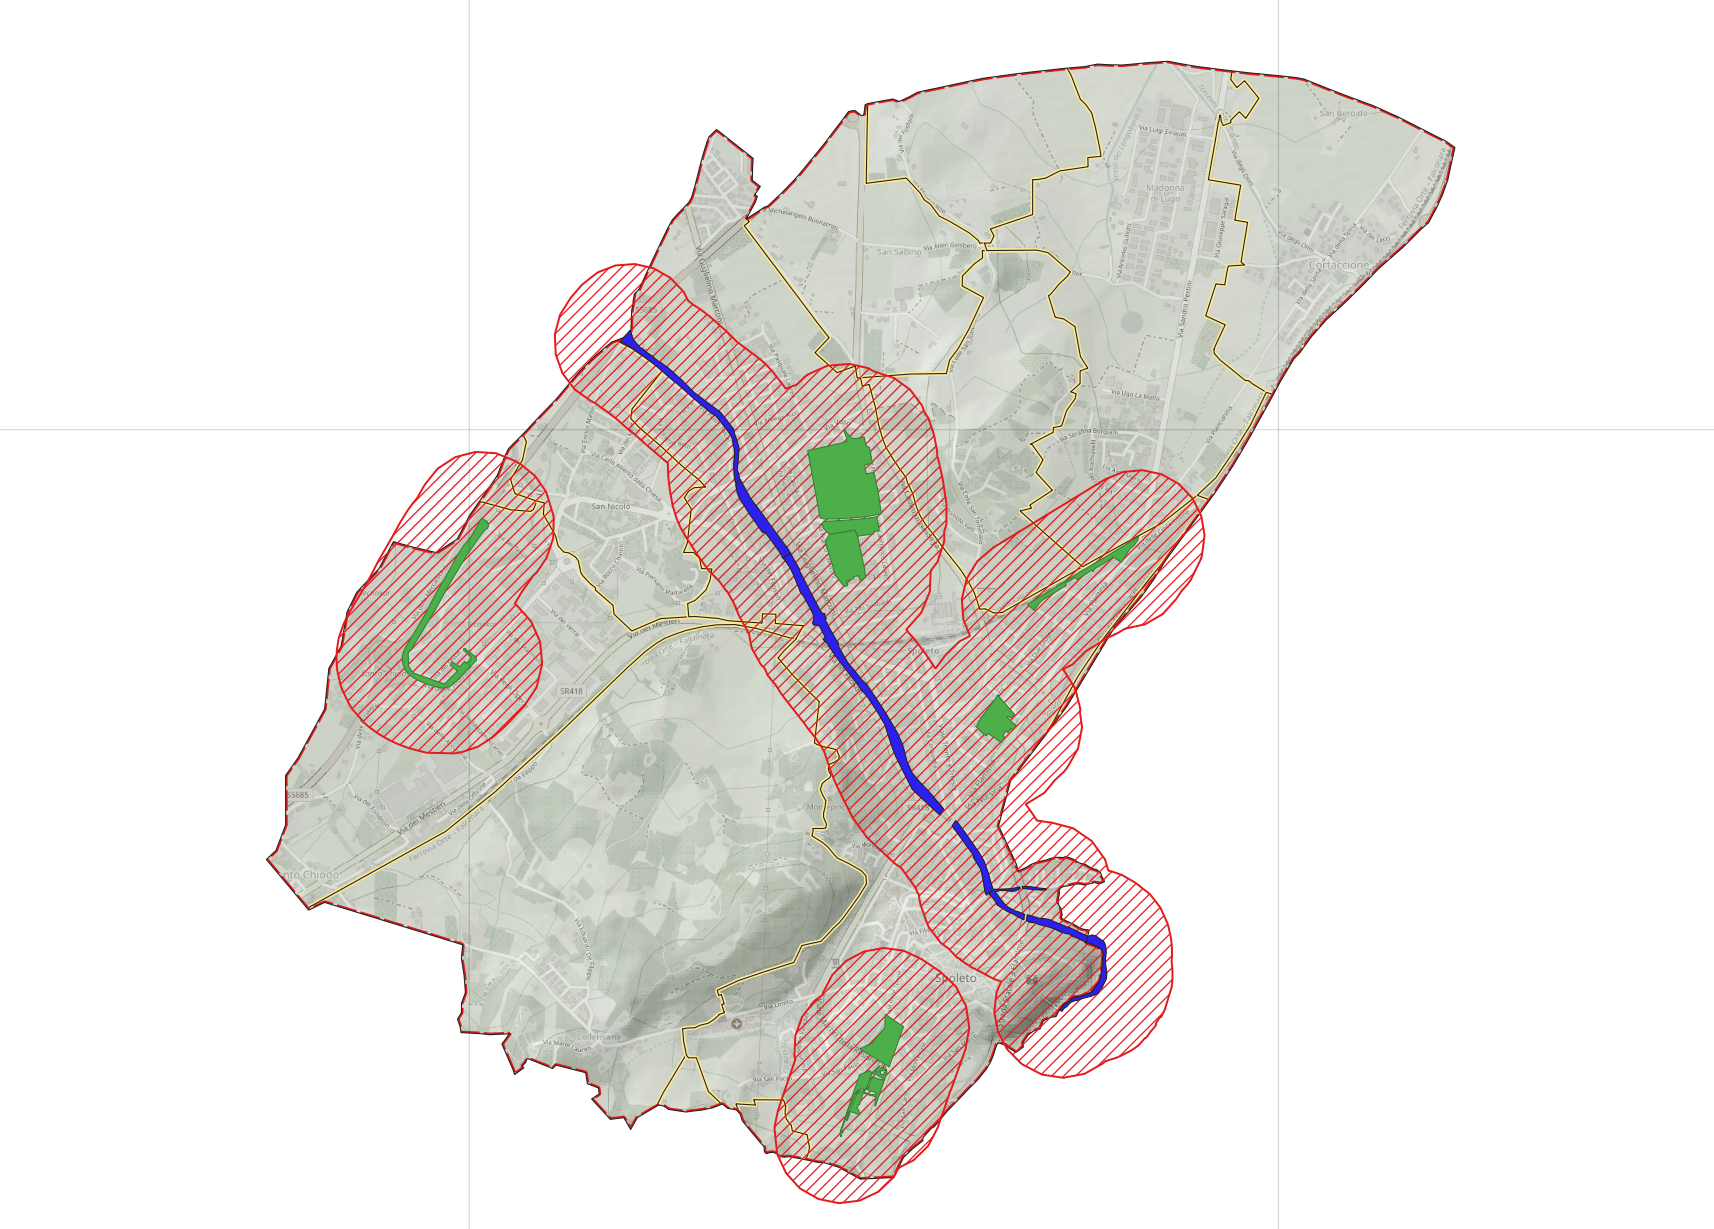
\includegraphics[width=\linewidth]{./figs/rule_buf300_1ha} 

}

\caption{In rosso buffer di 300 m intorno alle aree verdi urbane di natura pubblica.}\label{fig:rulebuf300}
\end{figure}

\begin{figure}

{\centering 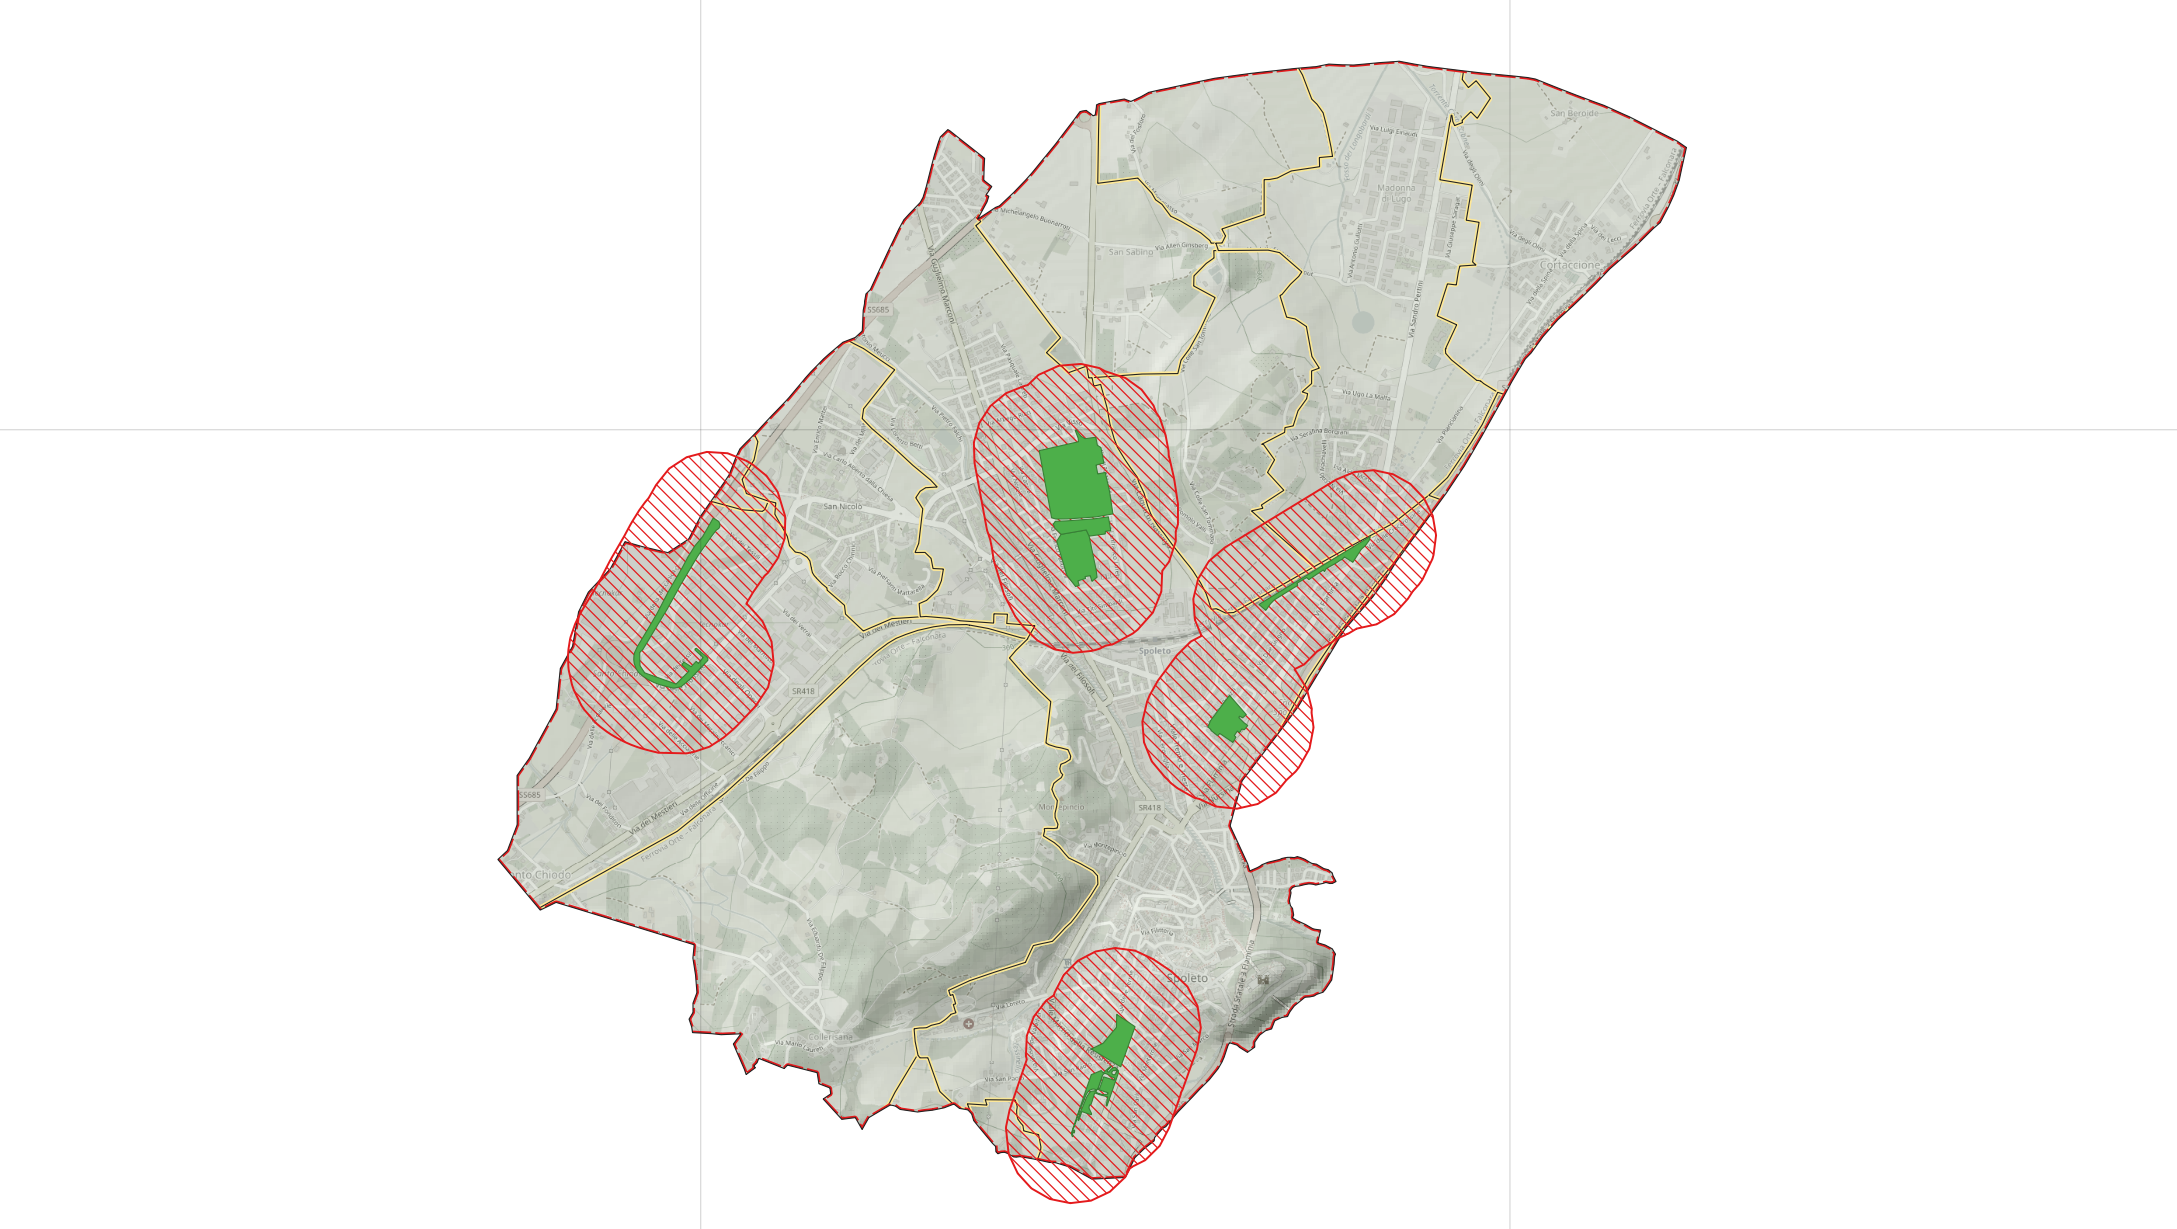
\includegraphics[width=\linewidth]{./figs/rule_buf300_1ha_noTess} 

}

\caption{In rosso buffer di 300 m intorno alle aree verdi urbane di natura pubblica senza l'inclusione del corridoio fluviale del torrente Tessino.}\label{fig:rulebuf300NT}
\end{figure}

\subsection{Priorità di conservazione e connessione (Marxan)}\label{priorituxe0-di-conservazione-e-connessione-marxan}

=={[}da completare primo step{]}==

\section{Risultati del sondaggio Greenway}\label{risultati-del-sondaggio-greenway}

=={[}da elaborare{]}==

\chapter{Indirizzi per la gestione e la progettazione}\label{indirizzi-per-la-gestione-e-la-progettazione}

=={[}testo di raccordo: dalle analisi emerge che\ldots{} quindi si propongono le seguenti azioni{]}==

\section{Analisi dei pattern morfologici spaziali dell'area di Piazza d'Armi e delle zone limitrofe}\label{analisi-dei-pattern-morfologici-spaziali-dellarea-di-piazza-darmi-e-delle-zone-limitrofe}

Al fine di valutare il contributo dell'area di Piazza d'Armi agli obiettivi di rinaturalizzazione e contrasto al consumo di suolo previsti dal Fondo Regionale Umbro, è stata condotta un'analisi morfologica spaziale mediante metodologia MSPA (Morphological Spatial Pattern Analysis). Questo approccio consente di esaminare il ruolo ecologico dell'area e di quantificare il suo potenziale nel contesto della rete ecologica locale (REL) e quella regionale (RERU).

\subsection{Approccio metodologico e basi dati}\label{approccio-metodologico-e-basi-dati-1}

Nel dettaglio, l'analisi MSPA è stata utilizzata per valutare la connettività ecologica e la struttura del paesaggio impiegando due distinti buffer intorno all'area di Piazza d'Armi: il primo buffer di 1 km è stato utile per definire le caratteristiche di contesto immediato, il secondo di 2 km è stato funzionale alla valutazione del grado di biopermeabilità del territorio circostante e del ruolo dell'area all'interno della rete ecologica locale. In questo modo è stato possibile evidenziare come l'area di indagine si inserisca nei corridoi di connettività esistenti e contribuisca alla funzionalità ecosistemica a scala di paesaggio. In linea generale, il framework metodologico della metodica MSPA si basa su un sistema di operatori matematico-morfologici progettati per caratterizzare le geometrie spaziali e le relazioni di connettività presenti nella carta di uso del suolo. Si tratta di un processo di segmentazione dei dati di input che nel caso specifico è stato basato sui risultati dell'elaborazione della carta geobotanica regionale dell'Umbria, aggiornata alla scala comunale nell'ambito delle attività della convenzione ``Studio della rete ecologica applicato al potenziamento della connettività del territorio spoletino attraverso esperienze pilota di gestione e interventi infrastrutturali su specifiche specie target e ambiti prioritari, oltre a percorsi didattico informativo promozionali'' con l'Università degli Studi di Perugia.

Dall'esame della carta riportata in fig.~\ref{fig:mappaPaceBuf1k} e dalla distribuzione delle diverse classi MSPA nel territorio ricompreso nel buffer di 1 km (Fig. \ref{fig:mappaPacePlotBuf1k}) emerge che circa il 75\% di questo territorio si articola in:

\begin{itemize}
\tightlist
\item
  Bridge (69 ha): è la classe dominante con la maggiore estensione (43\%). A questa classe corrisponde la categoria dei ``ponti'', generalmente definiti come corridoi ecologici, che connettono aree core, fondamentali per la connettività della rete ecologica. In particolare, è evidente che ad assolvere questa funzione è soprattutto l'ecotono ripario del torrente Tessino e le sue zone prossimali a occidente, mentre nella porzione orientale tale funzione è svolta dall'insieme degli elementi dell'ecosistema di colle San Tommaso.
\item
  Islet (26 ha): frammenti isolati di habitat, abbastanza presenti nell'area in esame e che soprattutto nella porzione settentrionale potrebbero svolgere una funzione importante per garantire ulteriore connettività verso l'area della Greenway.
\item
  Branch (25 ha): ramificazioni che si estendono dalle aree core, ma con una sola connessione.
  Altre categorie presenti nell'area (per una superficie complessiva pari a circa il 25\%) sono:
\item
  Edge (16 ha): bordi delle aree core, zone di transizione, note anche come aree ecotonali.
\item
  Aree Core (14 ha): aree centrali di habitat. Ad assolvere questa funzione potrebbe essere solo l'area di Piazza d'Armi e le aree sportive contigue, attraverso la riprogettazione degli spazi e il miglioramento della loro funzionalità ecologica.
\item
  Loop (10 ha): connessioni che creano percorsi circolari intorno a singole aree core.
  In sintesi, questa configurazione suggerisce un sistema caratterizzato da una notevole frammentazione, dove le connessioni ecologiche (Bridge) prevalgono sulle aree core, ma con una notevole potenzialità che potrebbe essere sviluppata mettendo a sistema tutti gli elementi naturali già esistenti.
\end{itemize}

\begin{figure}

{\centering 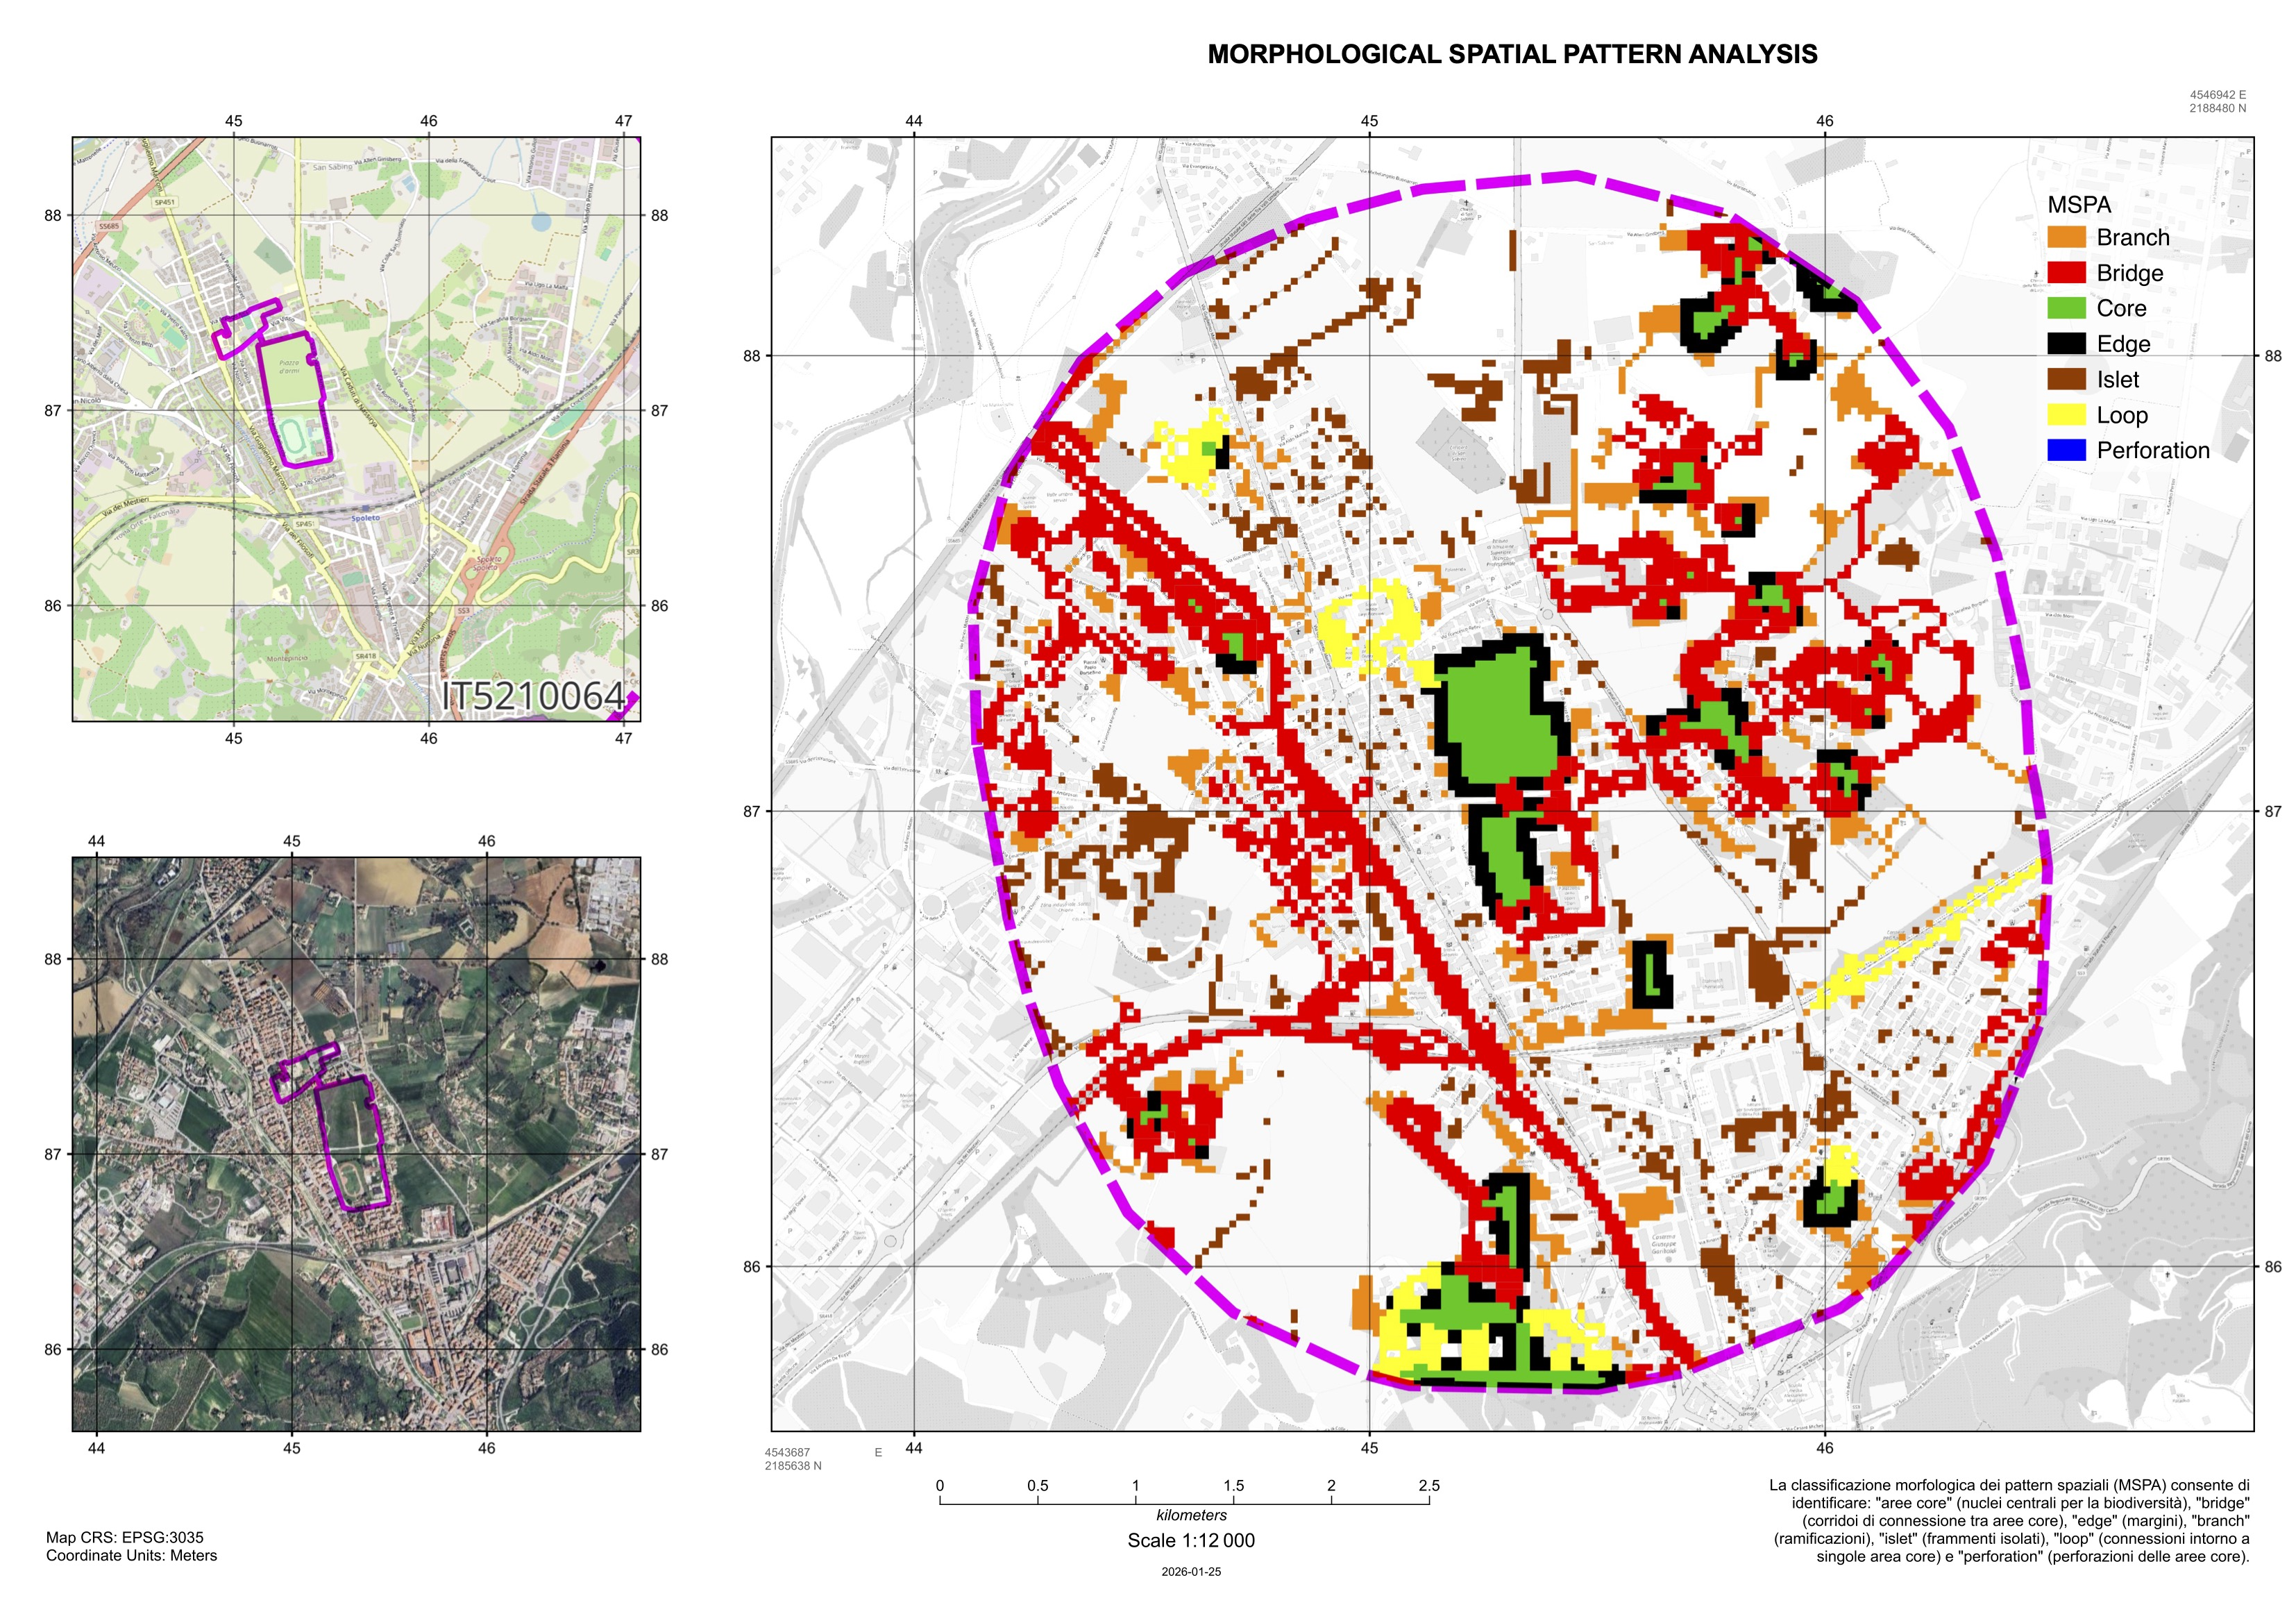
\includegraphics[width=\linewidth]{./figs/paceMappaBuf1k} 

}

\caption{Mappa del territorio ricompreso nel buffer di 1 km dall’area di indagine. A destra la riclassificazione del territorio secondo il metodo MSPA.}\label{fig:mappaPaceBuf1k}
\end{figure}

\begin{figure}

{\centering 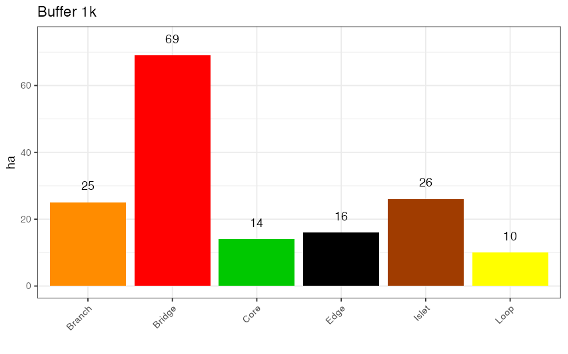
\includegraphics[width=\linewidth]{./figs/paceMspaPlot1k} 

}

\caption{Distribuzione delle classi MSPA nel territorio ricompreso nel buffer di 1 km dall’area di indagine.}\label{fig:mappaPacePlotBuf1k}
\end{figure}

Allargando il campo di valutazione e confrontando le analisi MSPA con buffer diversi (1 km vs 2 km), è possibile far emergere interessanti dinamiche sulla struttura ecologica del territorio alle due diverse scale spaziali \ref{fig:mappaPaceBuf2k}.

I principali cambiamenti tra il contesto immediato, rappresentato dal buffer 1k, e quello di scala locale proprio del buffer 2k (\ref{fig:mappaPacePlotBuf2k}) sono:

\begin{itemize}
\tightlist
\item
  Aree Core (da 14 a 167 ha): estendendo l'area di indagine, molte aree classificate come aree core si aggiungono all'area di Piazza d'Armi. Questo indica che il territorio presenta un buon potenziale di habitat, soprattutto se si tiene conto che nella porzione meridionale è presente il sito Natura 2000 IT5210064 -- Monteluco di Spoleto insieme alle aree pedemontane della dorsale appennica, mentre a nord si trova il sistema ecologico della Greenway. Da notare anche la vicinanza dell'area umida dei Pozzaccheri di Madonna di Lugo nell'area orientale che costituisce un'importante stepping stone per la biodiversità locale.
\item
  Bridge (da 69 a 139 ha): le porzioni di territorio capaci di svolgere questa importante funzione ecologica nel passaggio di scala di buffer raddoppiano. Infatti, i corridoi ecologici si rafforzano, sebbene il nucleo centrale, rappresentato dal corridoio del torrente Tessino e dagli ecosistemi di colle San Tommaso, rimanga invariato. È da sottolineare che il corridoio ecologico tra il sistema di colle San Tommaso e l'area di Piazza d'Armi si presenta particolarmente stretto, rendendo indispensabile la salvaguardia del varco esistente per garantire la continuità della rete ecologica.
\item
  Edge (da 16 a 93 ha): aumentando le aree core aumentano di conseguenza anche le zone di transizione attorno alle aree più estese.
\item
  Islet (da 26 a 80 ha): anche i frammenti isolati aumentano, ma proporzionalmente in misura inferiore rispetto ad altre classi (passano infatti dal 16 al 14\%), mantenendo un livello di frammentazione contenuto.
\item
  Perforation (da 0 a 11 ha): a questa scala compaiono alcune ``perforazioni'' non particolarmente critiche nelle aree core in corrispondenza dell'area pedemontana appenninica.
\item
  Branch e Loop: mantengono valori di superficie sostanzialmente immutati, rispettivamente 10 e 7\%.
\end{itemize}

\begin{figure}

{\centering 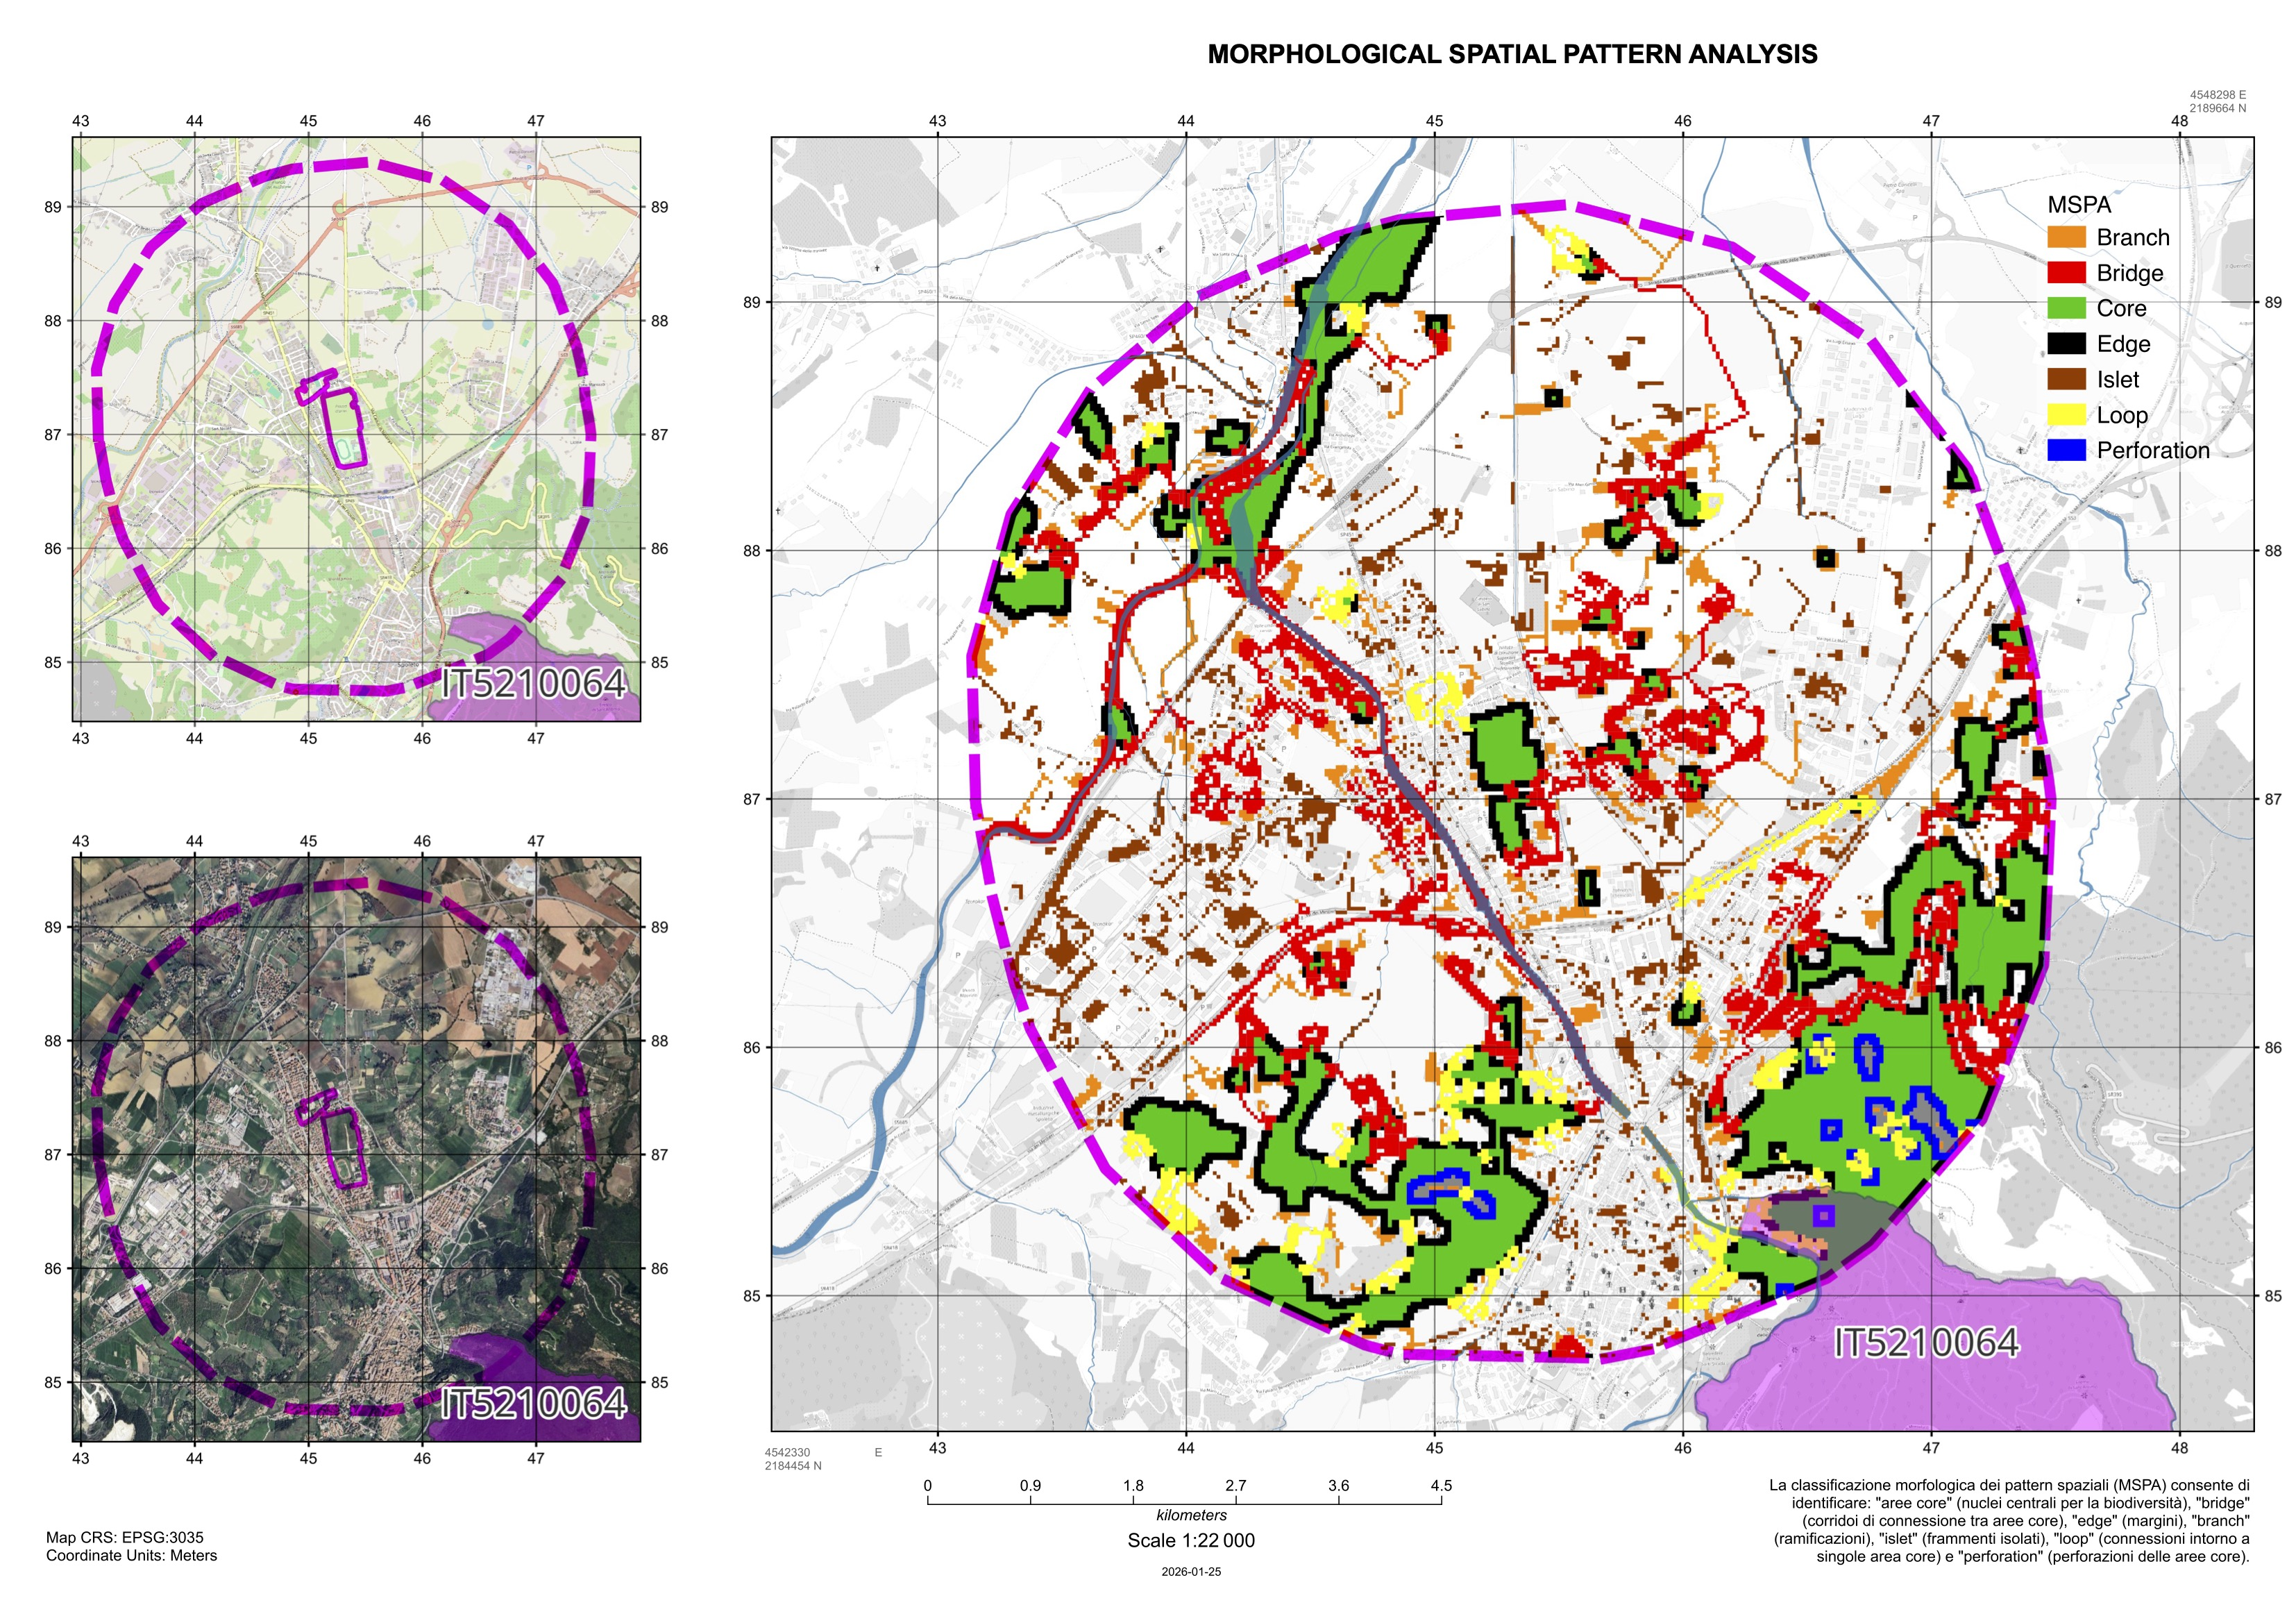
\includegraphics[width=\linewidth]{./figs/paceMappaBuf2k} 

}

\caption{Mappa del territorio ricompreso nel buffer di 2 km dall’area di indagine. A destra la riclassificazione del territorio secondo il metodo MSPA.}\label{fig:mappaPaceBuf2k}
\end{figure}

\begin{figure}

{\centering 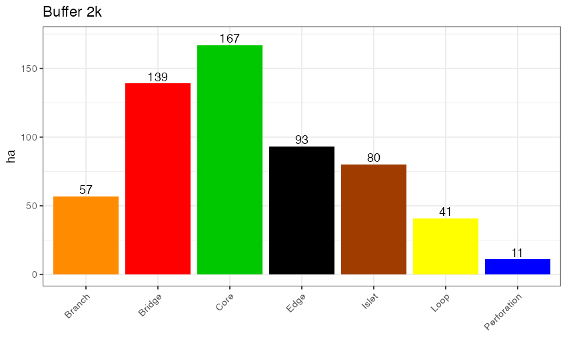
\includegraphics[width=\linewidth]{./figs/paceMspaPlot2k} 

}

\caption{Distribuzione delle classi MSPA nel territorio ricompreso nel buffer di 2 km dall’area di indagine.}\label{fig:mappaPacePlotBuf2k}
\end{figure}

\subsection{Considerazioni conclusive}\label{considerazioni-conclusive}

Dall'analisi dei pattern spaziali emerge la rilevanza ecologica dell'area di Piazza d'Armi nella creazione di un sistema verde multifunzionale ad uso pubblico, capace di integrare obiettivi di conservazione della biodiversità, fruizione sociale e contrasto al degrado del suolo. L'area, per la sua configurazione e posizione strategica, si caratterizza come elemento chiave nel contesto della rete ecologica locale e in quella regionale attraverso la connessione dell'area Natura 2000 IT5210064 -- Monteluco di Spoleto con la Greenway -- Valle Spoletana. Inoltre, il miglioramento delle sue potenzialità ecologiche potrebbe fornire un notevole contributo alla rigenerazione ambientale e alla riduzione della frammentazione a scala di paesaggio urbano e periurbano. Di tutto ciò potrebbero beneficiare sia gli ecosistemi e la biodiversità locale sia la comunità spoletina che, in una visione olistica One Health fondata sul riconoscimento dell'interconnessione indissolubile tra salute umana, animale ed ecosistemica, sottolinea come il ripristino ecologico delle aree urbane rappresenti un investimento strategico per il benessere collettivo.

In questa prospettiva, la figura \ref{fig:parcoPace} illustra un'ipotesi semplificata di assetto e riorganizzazione dell'area quale parco urbano multifunzionale (futuro Parco della Pace) con percorsi pedonali, aree alberate e siepi, concepite per coniugare l'erogazione dei servizi ecosistemici con spazi dedicati al tempo libero, alla socializzazione e all'educazione ambientale. Questa configurazione consente di massimizzare la permeabilità della matrice urbana e di rafforzare la funzione di cerniera ecologica dell'area tra il centro urbano e la zona periurbana.

\begin{figure}

{\centering 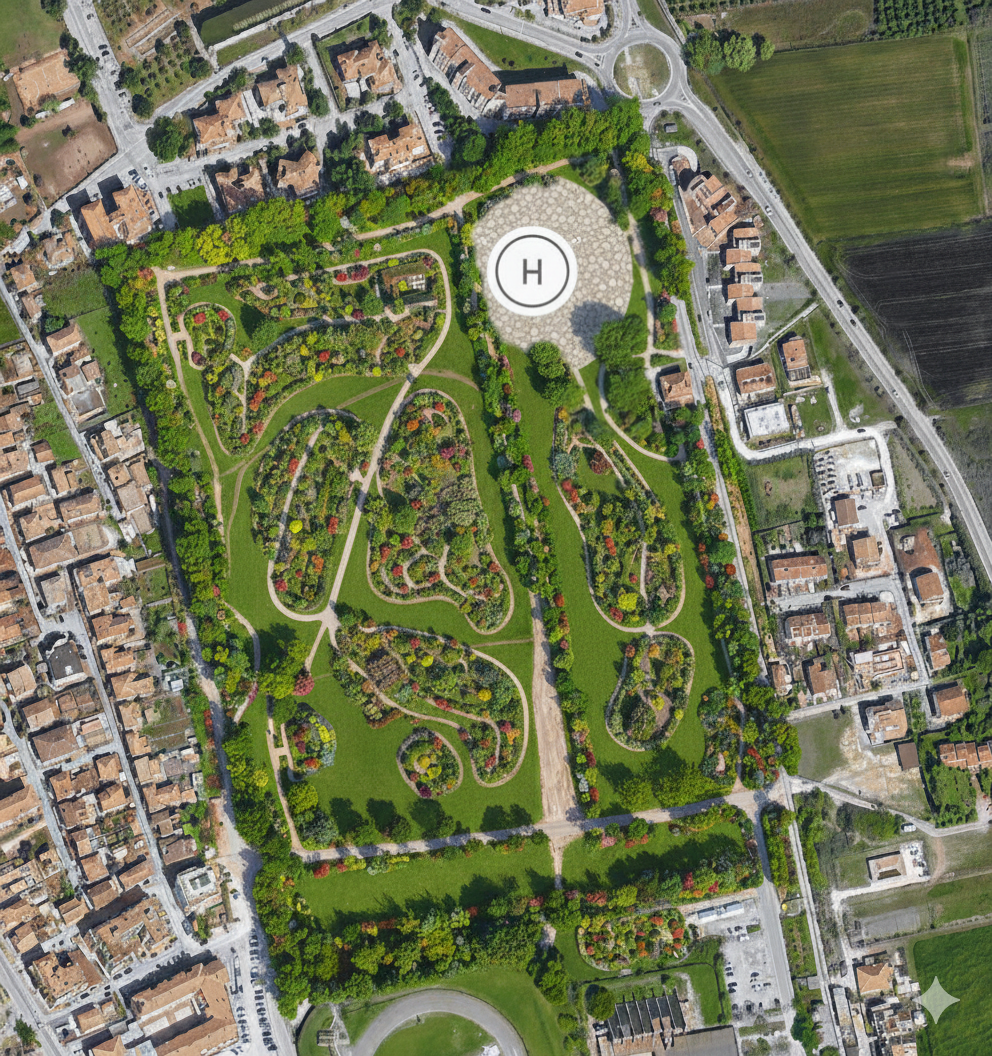
\includegraphics[width=\linewidth]{./figs/parcoPace_idea} 

}

\caption{A titolo esemplificativo, la Figura 5.5 illustra un'ipotesi di riorganizzazione spaziale dell'ambito come parco urbano (futuro Parco della Pace).}\label{fig:parcoPace}
\end{figure}

\section{Prati urbani}\label{prati-urbani}

I prati urbani (urban lawns) rappresentano una delle componenti più diffuse delle infrastrutture verdi urbane a livello globale, arrivando a coprire fino al 70\% delle aree verdi cittadine all'interno di parchi pubblici, giardini privati, campus, aree sportive e margini stradali (Ignatieva et al.~2020; Hedblom et al.~2017). Storicamente sono stati concepiti per scopi estetici, ricreativi e culturali, ma allo stesso tempo i prati urbani forniscono importanti servizi ecosistemici, tra cui il mitigamento dell'isola di calore, il sequestro del carbonio, la filtrazione dell'acqua, la creazione di spazi di habitat per la biodiversità e di aggregazione per i cittadini (Dushkova \& Ignatieva 2020; Strohbach et al.~2012). Tuttavia, la loro gestione convenzionale, caratterizzata da sfalci intensivi, irrigazione e, talvolta, dall'impiego di fertilizzanti e fitofarmaci, comporta elevati costi economici e significativi impatti ambientali. Di fronte a queste evidenze, emerge quindi la necessità di ripensare la gestione di questi spazi attraverso le Nature-based Solutions e gli approcci di rewilding urbano. In questa prospettiva, la transizione verso forme di gestione ecologica si configura come una soluzione strategica per ripristinare le funzioni ecosistemiche, incrementare la biodiversità e rafforzare la resilienza delle comunità urbane (Nesshöver et al.~2017; Solcerova et al.~2023).
Ovviamente quando si tratta di ripensare alla loro gestione, non si tratta di abbandonare la manutenzione, ma di ricondurla a pratiche differenziate, in cui frequenza, altezza, periodo e porzione di superficie sfalciata sono variabili da calibrare in funzione dell'uso e del ruolo ecologico di ciascuna area (Kirby et al.~2025; Dushkova e Ignatieva 2025). L'idea di fondo è che una parte degli spazi verdi, soprattutto quelli in cui l'uso ricreativo è marginale, possa svolgere funzioni di habitat con costi gestionali inferiori, senza dover sostituire il prato con l'impianto di nuove specie.

I benefici ecologici della riduzione degli sfalci sono ampiamente documentati.

Nei prati urbani passati da sfalci ogni poche settimane a uno o due tagli per stagione, entro sei anni la ricchezza floristica è risultata superiore del 30\% rispetto ai prati gestiti in modo intensivo, con una composizione che si sposta da specie comuni e tolleranti lo sfalcio verso specie tipiche dei prati (Sehrt et al.~2020). Chollet et al.~(2018) riportano un aumento della diversità tassonomica, funzionale e filogenetica delle piante. Gli effetti riguardano anche gli insetti e altri artropodi: una meta-analisi su contesti urbani temperati indica che la riduzione dello sfalcio ha un effetto positivo medio sull'abbondanza (g = 0,54) e ampio sulla ricchezza di taxa (g = 1,25), mentre i prati curati favoriscono in modo sproporzionato le specie opportuniste e più antropofile (Proske et al.~2022). In un progetto sui prati per le farfalle (oltre 640 prati sfalciati solo in parte e al massimo tre volte l'anno), nove prati hanno mostrato biomassa e numero di specie di insetti più alti di nove prati intensivamente sfalciati, con la presenza di larve a indicare riproduzione in loco (Wintergerst et al.~2021).

La relazione tra sfalcio, biodiversità e risorse per gli impollinatori non è però lineare. In un esperimento su sedici giardini del Massachusetts lo sfalcio ogni tre settimane ha prodotto fino a 2,5 volte più fiori rispetto alle altre frequenze, ma l'abbondanza massima di api selvatiche si è registrata con sfalci ogni due settimane, con ricchezza ed equitabilità più basse (Lerman et al.~2018). L'obiettivo, quindi, non è «non sfalciare», ma calibrare questa tipologie d'intervento.

Naturalmente, la riduzione degli interventi ha anche una ricaduta economica. In un caso studio canadese il passaggio da 15 a 10 sfalci annui nelle aree molto frequentate, e da tre a uno in quelle poco frequentate, è stato stimato in un risparmio del 36\% dei costi di manutenzione, considerando i soli costi contrattuali. Lo stesso lavoro riporta che la gestione intensiva favorisce infestanti e parassiti dei prati, e che un'infestante allergenica come l'ambrosia (\emph{Ambrosia artemisiifolia}) può essere contenuta riducendo la frequenza di sfalcio (Watson et al.~2020).

La riuscita di queste strategie dipende in larga misura dall'accettazione da parte dei cittadini. Per evitare che un prato a sfalcio ridotto venga percepito come un'area abbandonata o degradata, è fondamentale applicare i «segnali di cura» (\emph{cues to care}, introdotti da Nassauer nel 1995), ovvero elementi di disegno e manutenzione perimetrale (come fasce sfalciate lungo i bordi) che rendano esplicita l'intenzionalità gestionale. Le evidenze di gradimento sono incoraggianti: in un parco inglese le strisce non sfalciate hanno avuto circa tre volte più fiori e cinque volte più insetti visitatori di fiori rispetto alle strisce sfalciate regolarmente, e il 97\% dei visitatori intervistati si è detto favorevole a favorire insetti e fiori spontanei (Garbuzov et al.~2015). Riscontri analoghi emergono dai lavori di Norton et al.~(2019), che evidenziano una maggiore soddisfazione dei residenti in presenza di coperture vegetali diversificate.

In sostanza, l'approccio per sua natura deve essere adattivo e spazialmente disaggregato. Aree sportive, percorsi e zone ad alta visibilità richiedono sfalci frequenti per garantire sicurezza e fruibilità, mentre i prati a sfalcio ridotto trovano collocazione ideale laddove la funzione ecologica può prevalere. L'organizzazione in un mosaico multifunzionale massimizza i benefici complessivi per la biodiversità (Norton et al.~2019).
Nel quadro normativo europeo, l'art. 8 del Regolamento (UE) 2024/1991 sulla ripristino della natura (Nature Restoration Law) impone che la superficie a verde e la copertura arborea urbana non diminuiscano rispetto ai livelli del 2024 entro il 2030, per poi registrare una crescita progressiva (ISPRA). Poiché i vincoli quantitativi devono essere supportati da una reale qualità ecologica, la gestione mirata dello sfalcio diventa uno strumento strategico fondamentale.

\subsection{Prato a sfalcio ridotto presso la Spoletosfera}\label{prato-a-sfalcio-ridotto-presso-la-spoletosfera}

Nel caso di Spoleto è stata avviata una sperimentazione presso l'area della Spoletosfera (Fig. \ref{fig:spoletoSferaSign}), in cui viene proposta una gestione sostenibile del patrimonio naturale cittadino con l'idea di arricchire gli habitat, incrementare gli impollinatori e tutelare la biodiversità, in particolare della piccola fauna. Nello stesso tempo con un riequilibrio delle diverse componenti ecologiche ci si attende un contenimento degli insetti antropofili, una mitigazione dell'isola di calore, grazie al miglioramento della ritenzione idrica dei suoli.

\begin{figure}

{\centering 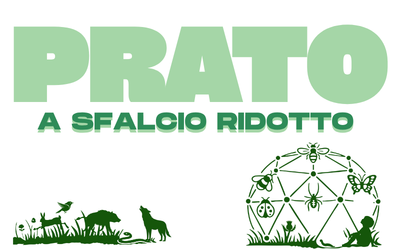
\includegraphics[width=\linewidth]{./figs/spoletoSfera_sign} 

}

\caption{Logo progettato per la segnaletica 'di cura' presso l'area della Spoletosfera.}\label{fig:spoletoSferaSign}
\end{figure}

Per la caratterizzazione della comunità entomologica presente nell'area a sfalcio ridotto, nel periodo primaverile è stata condotta una campagna di campionamento mirata a rilevare la ricchezza e la composizione dei taxa di insetti associati alla matrice erbacea. Il disegno di campionamento ha previsto l'individuazione di 6 transetti rappresentativi dell'area di studio (Fig. \ref{fig:spoletoSferaTransetti}). Per ciascun transetto la raccolta del materiale entomologico è stata eseguita mediante l'impiego di un retino da sfalcio (sweep net), adottando una metodologia di tipo semiquantitativo basata sullo sforzo temporale (standardizzato in circa 5 minuti di sfalcio attivo per transetto). Tutti i campioni raccolti sul campo sono stati immediatamente stoccati, catalogati e trasferiti in laboratorio per le fasi successive di lavorazione consistenti in: i) sorting ed estrazione: separazione del materiale biologico dai detriti vegetali e smistamento degli esemplari in base ai principali gruppi morfo-funzionali; ii) fissazione e conservazione dei reperti in soluzione alcolica (alcool etilico al 70\%), predisponendo il materiale per le successive analisi e determinazioni tassonomiche di dettaglio per un riconoscimento tassonomico a livello di famiglia, genere o specie.

\begin{figure}

{\centering 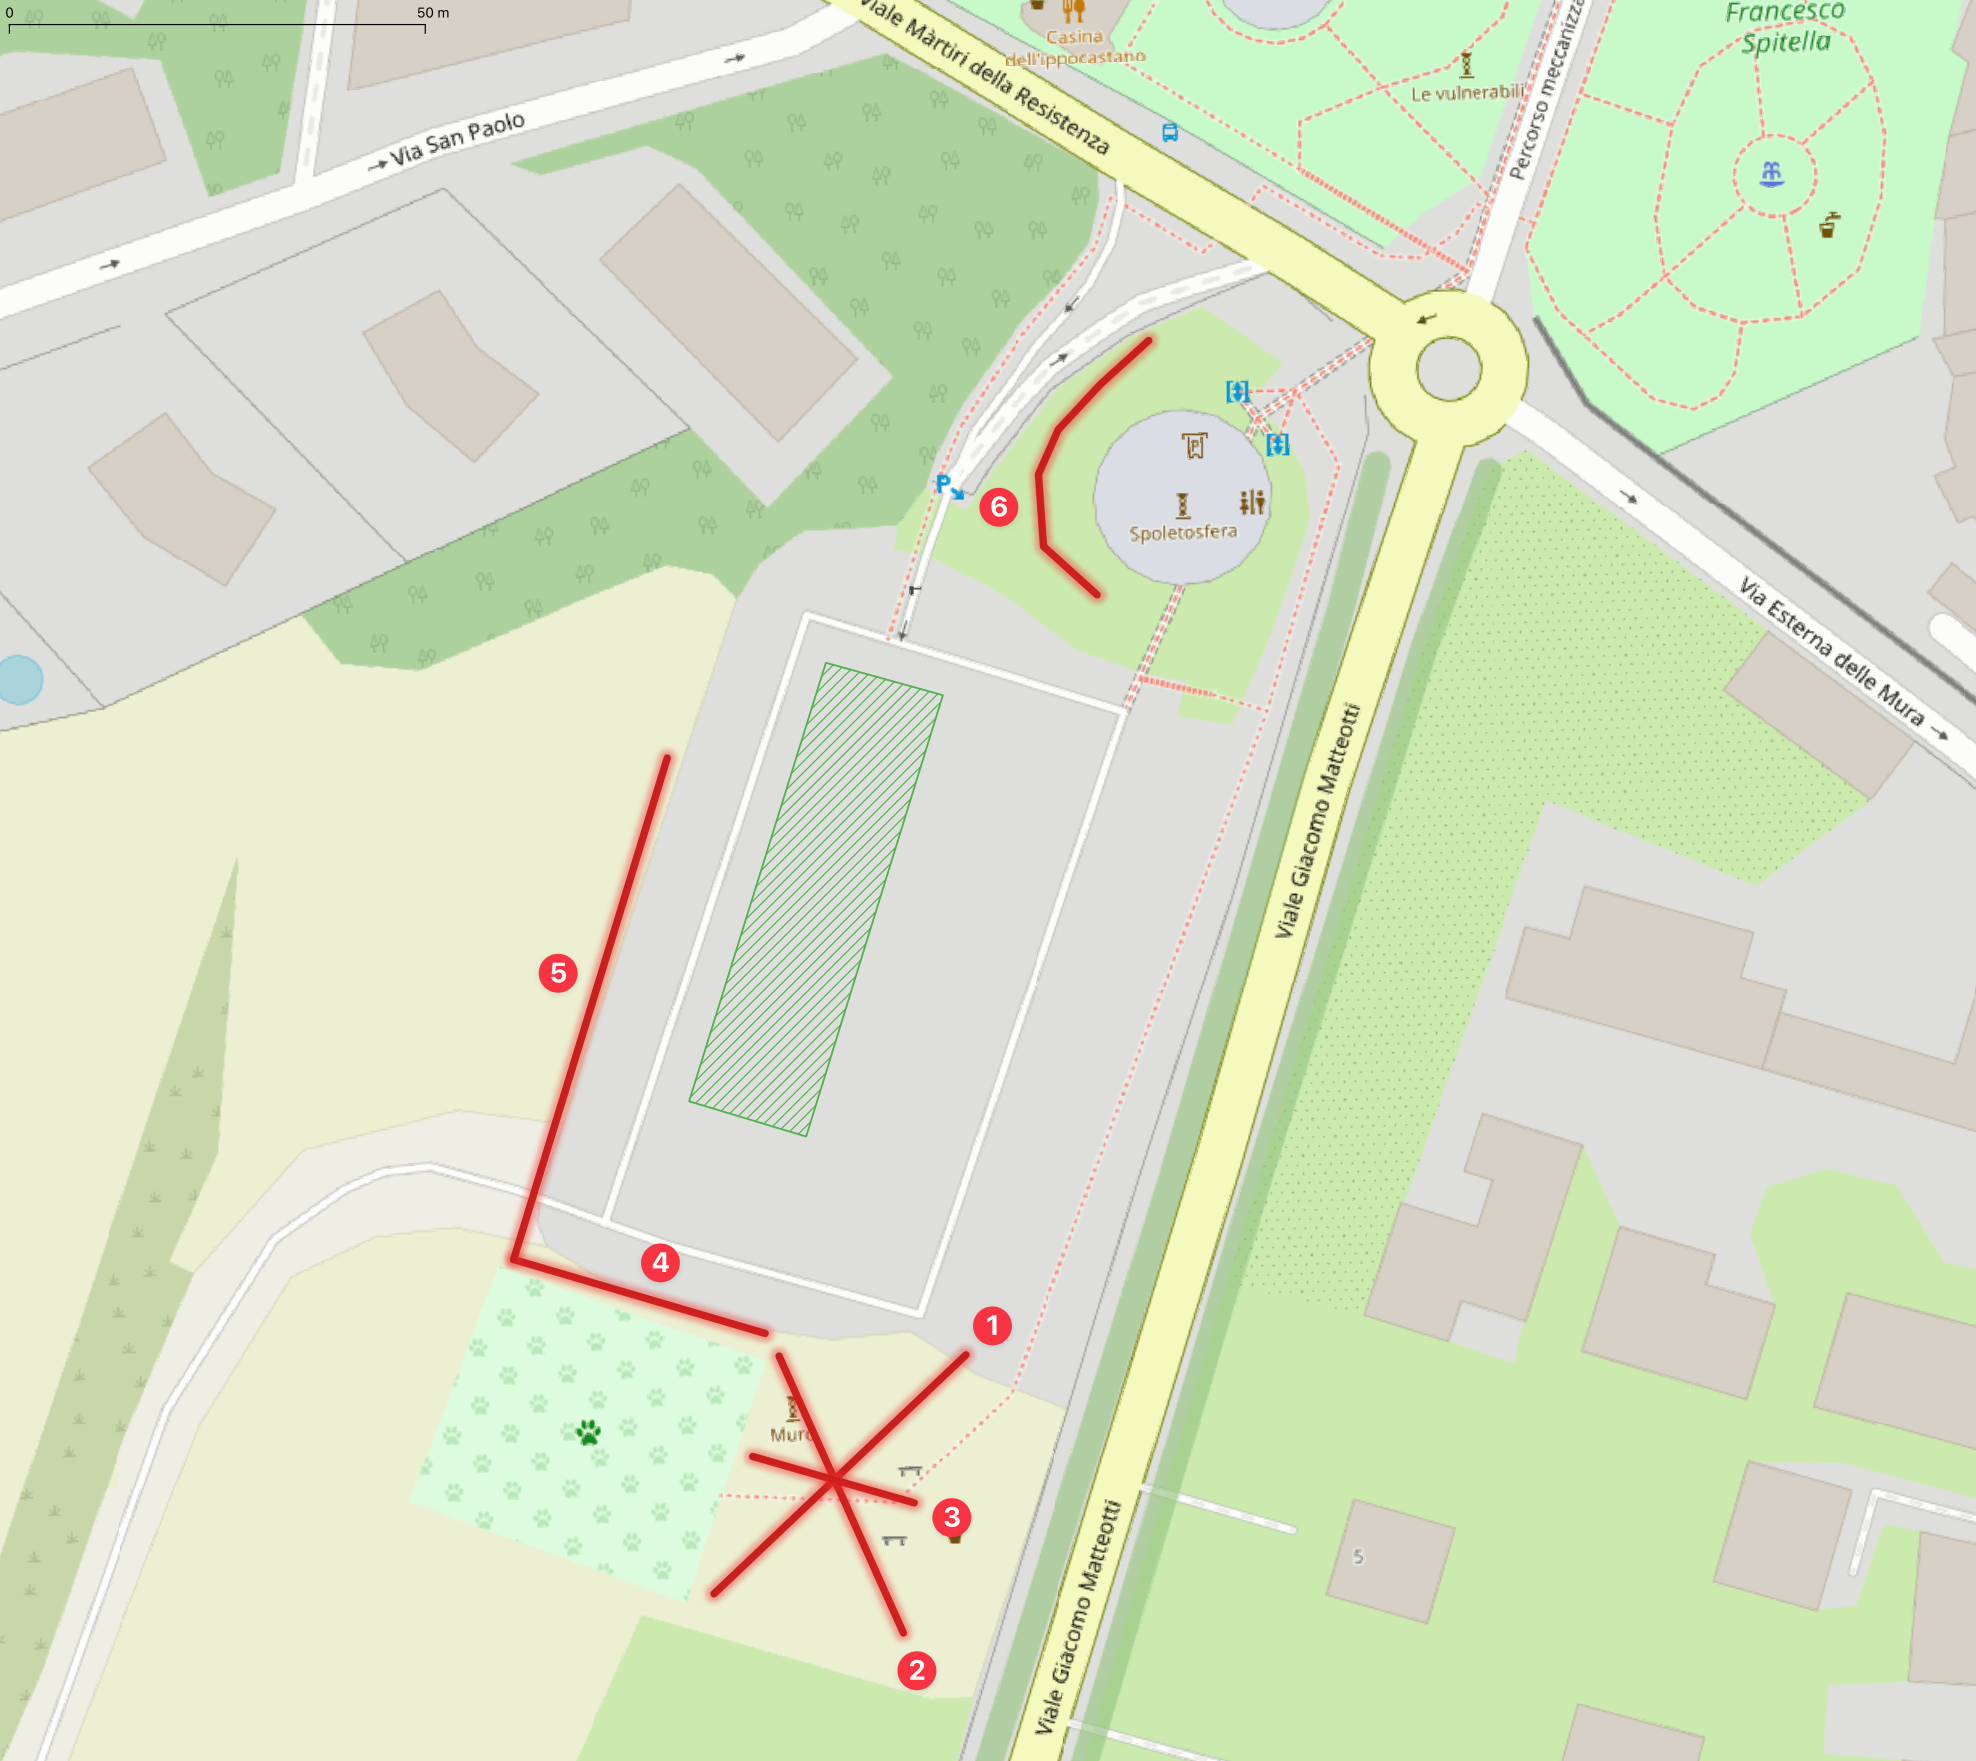
\includegraphics[width=\linewidth]{./figs/spoletoSfera_transetti} 

}

\caption{Transetti del monitoraggio entomologico presso l'area della Spoletosfera.}\label{fig:spoletoSferaTransetti}
\end{figure}

\subsection{Risultati preliminari}\label{risultati-preliminari}

L'efficacia del prato a sfalcio ridotto nella promozione della biodiversità è resa evidente dal confronto visivo tra la composizione dei campioni raccolti nei due differenti regimi gestionali (Fig. \ref{fig:sfalcioContinuativo} - 1 e 2) e in un prato naturale (Fig. \ref{fig:sfalcioContinuativo} - 3). Mentre nel prato soggetto a sfalcio continuativo ed intensivo la comunità di insetti risulta fortemente impoverita e dominata da poche specie opportuniste e tolleranti il disturbo frequente, l'area a sfalcio ridotto mostra una sensibile diversificazione dei gruppi tassonomici. In quest'ultimo contesto si osserva non solo un incremento generale dell'abbondanza di individui, ma soprattutto una spiccata ricchezza di taxa guida, tra cui impollinatori (Imenotteri e Lepidotteri), Ortotteri, Eterotteri e Coleotteri predatori, a conferma del ruolo di refugium ecologico svolto dalle superfici a gestione differenziata.

\begin{figure}

{\centering 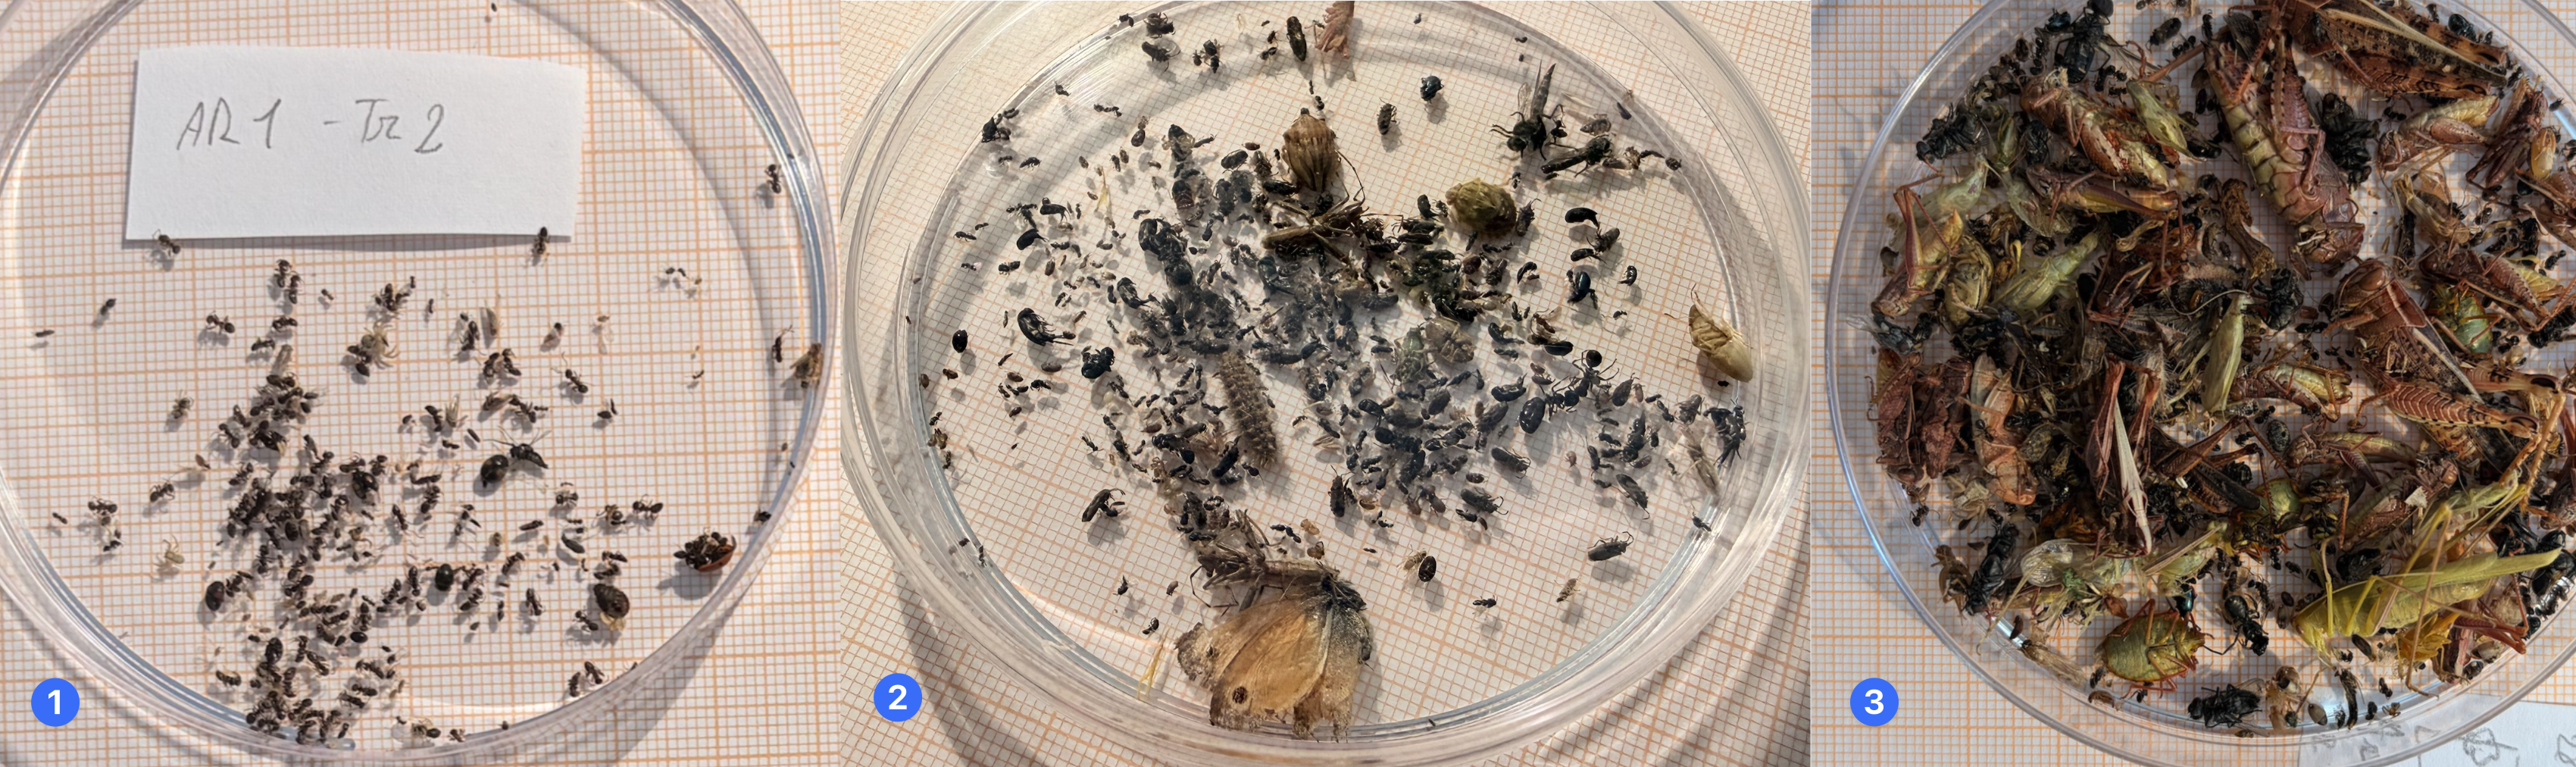
\includegraphics[width=\linewidth]{./figs/prato_sampling2026} 

}

\caption{In 1 e 2 i campioni raccolti durante il monitoraggio entomologico presso l'area della Spoletosfera. In 3 il risultato dello stesso sforzo di campionamento in un prato naturale periurbano.}\label{fig:sfalcioContinuativo}
\end{figure}

Sebbene la determinazione tassonomica di dettaglio sia tuttora in corso d'opera e richieda le tempistiche necessarie alla corretta identificazione dei singoli esemplari, le differenze tra i contesti appaiono già estremamente evidenti. I dati preliminari evidenziano uno scarto netto non solo in termini di ricchezza specifica, ma anche di abbondanza numerica e biomassa totale a favore delle superfici a sfalcio ridotto.
Parallelamente al monitoraggio entomologico, un gruppo di lavoro botanico sta completando l'elaborazione dei dati floristici rilevati nel medesimo periodo di campionamento (Fig. \ref{fig:sfalcioStudenti}). L'integrazione di tali banche dati permetterà di analizzare in modo combinato le relazioni tra la componente floristica e quella faunistica associata. In un'ottica di pianificazione a scala urbana, sarebbe di rilevante interesse estendere la rete di monitoraggio ad altre aree della città, al fine di effettuare confronti spaziali e temporali più ampi e verificare la risposta della biodiversità in contesti urbani caratterizzati da differenti gradi di frammentazione e pressione antropica. Presso la Spoletosfera le attività di monitoraggio proseguiranno nei prossimi mesi per coprire l'intero ciclo stagionale e i risultati delle analisi integrate verranno disseminati non appena disponibili.

\begin{figure}

{\centering 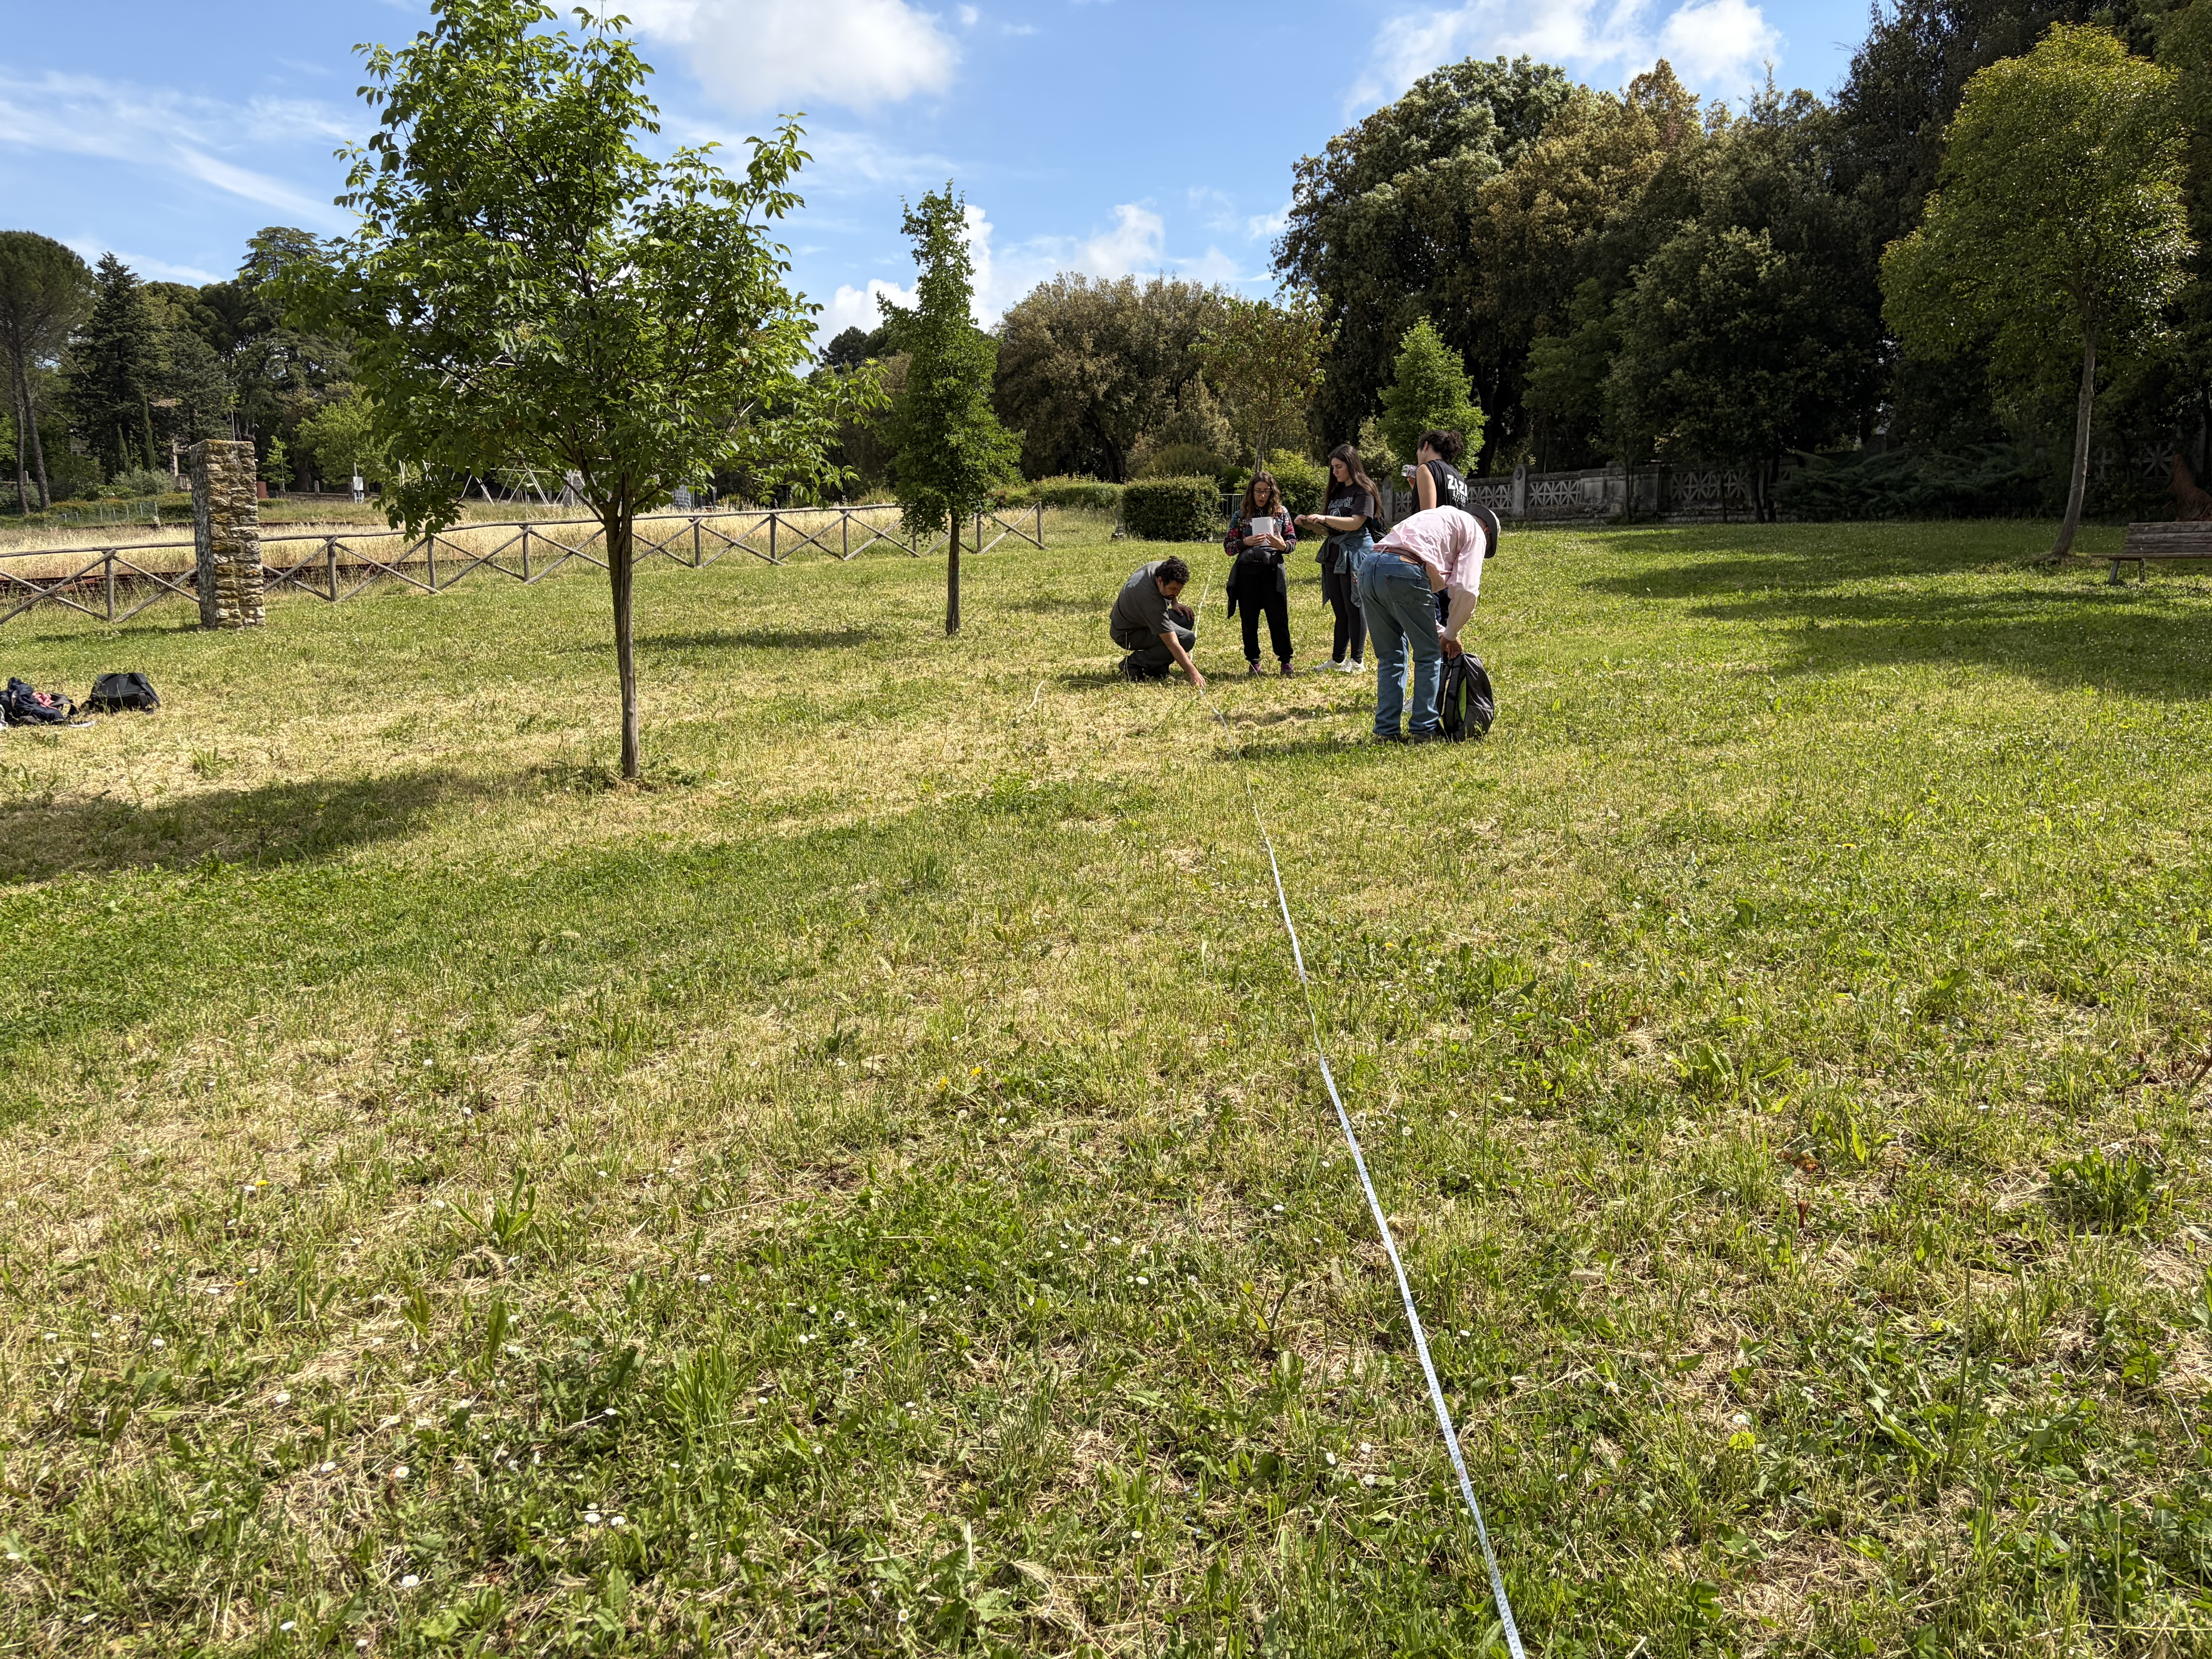
\includegraphics[width=\linewidth]{./figs/prato_studenti2026} 

}

\caption{Il gruppo botanico al lavoro presso l'area della Spoletosfera.}\label{fig:sfalcioStudenti}
\end{figure}

=={[}Nota sull'esperienza di Villa Redenta{]}==

\section{Schemi d'impianto}\label{schemi-dimpianto}

=={[}da completare{]}==

\section{Linee guida per la gestione del reticolo secondario (Abaco interventi)}\label{linee-guida-per-la-gestione-del-reticolo-secondario-abaco-interventi}

=={[}da collegare con il doc lifeIMAGINE{]}==

\chapter{Divulgazione scientifica}\label{divulgazione-scientifica}

\section{Eventi di disseminazione e campagna di citizen science}\label{eventi-di-disseminazione-e-campagna-di-citizen-science}

=={[}da inserire: attività di divulgazione scientifica, eventi e campagna di citizen science{]}==

\chapter{Considerazioni conclusive}\label{considerazioni-conclusive-1}

=={[}da completare{]}==

\chapter{Programmazione futura}\label{programmazione-futura}

\section{Piano delle attività}\label{piano-delle-attivituxe0}

=={[}da concordare{]}==

\chapter{Allegato I}\label{annexI}

\bibliography{references.bib}

\end{document}
